%
%---Beginning of Document---
%
% Use 1). latex ftof-nim.tex, 2). dvipdfm ftof-nim
%
%\RequirePackage{lineno}
\documentclass{elsart}
\usepackage[dvips]{color,graphics}
\usepackage[pdftex]{graphicx}
%\setcounter{footnote}{0}
\setcounter{tocdepth}{4}
%
\usepackage{lineno} 
\linenumbers

\begin{document}
\begin{frontmatter}

\title{The Forward Time-of-Flight System for CLAS12}

\author[JLab]{D.S. Carman\thanksref{corresponding}},
\author[USC]{R. Gothe},
\author[Glasgow]{L. Clark}
\author[INFN]{R. De Vita}
\author[JLab]{B. Miller}, and
\author[JLab]{C. Wiggins}

\address[JLab]{Thomas Jefferson National Accelerator Facility, Newport News, VA 23606, USA}
\address[USC]{University of South Carolina, Columbia, SC 29208, USA}
\address[Glasgow]{University of Glasgow, Glasgow G12 8QQ, United Kingdom}
\address[INFN]{INFN, Sezione di Genova, 16146 Genova, Italy}
\thanks[corresponding]{Corresponding author. Address: 12000 Jefferson Ave., Newport News, VA; 
e-mail: carman@jlab.org.}

\date{\today}

%\maketitle

\begin{abstract}
The Forward Time-of-Flight system for the large-acceptance CLAS12 spectrometer in Hall~B at the
Thomas Jefferson National Accelerator Facility is described. The system is positioned $\sim$6-7~m
from the beam-target interaction point and spans laboratory polar angles from $\sim 5^\circ \to 35^\circ$
and nearly the full azimuth. The system consists of 540 individual scintillation counters with double-ended
readout that range in length from 17~cm to 426~cm of discrete widths of 6~cm, 15~cm, and 22~cm, and of
discrete thicknesses of 5~cm and 6~cm. The effective counter time resolution for passing charged particles
varies from $\sim$50~ps for the shortest counters at small angles to $\sim$150~ps for the longest counters
at large angles. The detectors are part of the overall CLAS12 Forward Detector particle identification scheme
during offline event reconstruction and are part of the online data acquisition trigger to select final state
event topologies with charged hadrons.
\end{abstract}

\end{frontmatter}

PACS:29.40.Mc \\
Keywords: CLAS12, time of flight, plastic scintillator, particle identification
\newpage

\newpage
\tableofcontents

\vfil
\eject

\section{Overview of CLAS12}

The Thomas Jefferson National Accelerator Facility (JLab) recently completed a project to 
double the maximum energy of its electron accelerator from 6~GeV to 12~GeV. The experimental 
equipment in Hall~B forms the large-acceptance CLAS12 spectrometer that is designed to operate 
with beam energies up to 11~GeV at a nominal beam-target luminosity of 
$1 \times 10^{35}$~cm$^{-2}$s$^{-1}$ to allow for precision measurements of exclusive 
reactions with polarized beam and both unpolarized and polarized targets. This spectrometer is 
based on two superconducting magnets, a solenoid in the central region about the target and a 
toroid at forward angles.

The CLAS12 torus has a six-fold symmetry that divides the forward acceptance in the polar angle
range from 5$^\circ$ to 35$^\circ$ into six 60$^\circ$-wide sectors. It produces a field primarily in
the azimuthal direction. The torus $\int \!B d\ell$ field strength at its nominal full current is 2.8~T
at 5$^\circ$ and 0.5~T at 35$^\circ$. A set of three multi-layer drift chambers in each sector (before
the field, within the field, and after the field) and a forward micromegas vertex tracker are used for
charged particle tracking to measure momenta. Downstream of the torus each sector is instrumented
with a Cherenkov counter for $\pi/K$ separation (five sectors are instrumented with low threshold
gas Cherenkov counters and one sector is instrumented with a ring-imaging Cherenkov counter), three
planar layers of scintillation counters for charged particle timing measurements called the Forward
Time-of-Flight (FTOF) system, and an electromagnetic calorimeter system for electron and neutral
particle identification. Just upstream of the torus is a large-volume high-threshold gas Cherenkov
counter for electron identification and a tagging system to detect electrons and photons at scattering
angles below $5^\circ$.

The CLAS12 solenoid spans the central angular range from 35$^\circ$ to 125$^\circ$ and has a 
uniform 5~T central field. The solenoid serves to focus the low-energy M{\o}ller background down 
the beam pipe to the beam dump away from the acceptance of the spectrometer. The detectors mounted 
within the solenoid include a thick scintillation counter for neutron identification, a barrel of thin
scintillation counters for charged particle timing measurements, and a set of tracking detectors about the
target. Upstream of the solenoid, covering angles from 135$^\circ$ to 145$^\circ$ a wall of scintillation
counters is installed for additional neutron detection coverage.

Fig.~\ref{clas12-model} shows a model representation of CLAS12 to highlight its overall layout and scale.
The CLAS12 spectrometer was installed and instrumented in Hall~B in the period from 2012 to 2018. The
CLAS12 spectrometer took the place of the original CLAS spectrometer~\cite{clas-nim} that operated in
Hall~B in the period from 1997 to 2012 when it was decommissioned.

%%%%%%%%%%%%%%%%%%%%%%%%%%%%%%%%%%%%%%%%%%%%%%%%%%%%%%%%%
\begin{figure}[htbp]
\vspace{6.0cm}
\begin{picture}(50,50) 
\put(20,250)
{\hbox{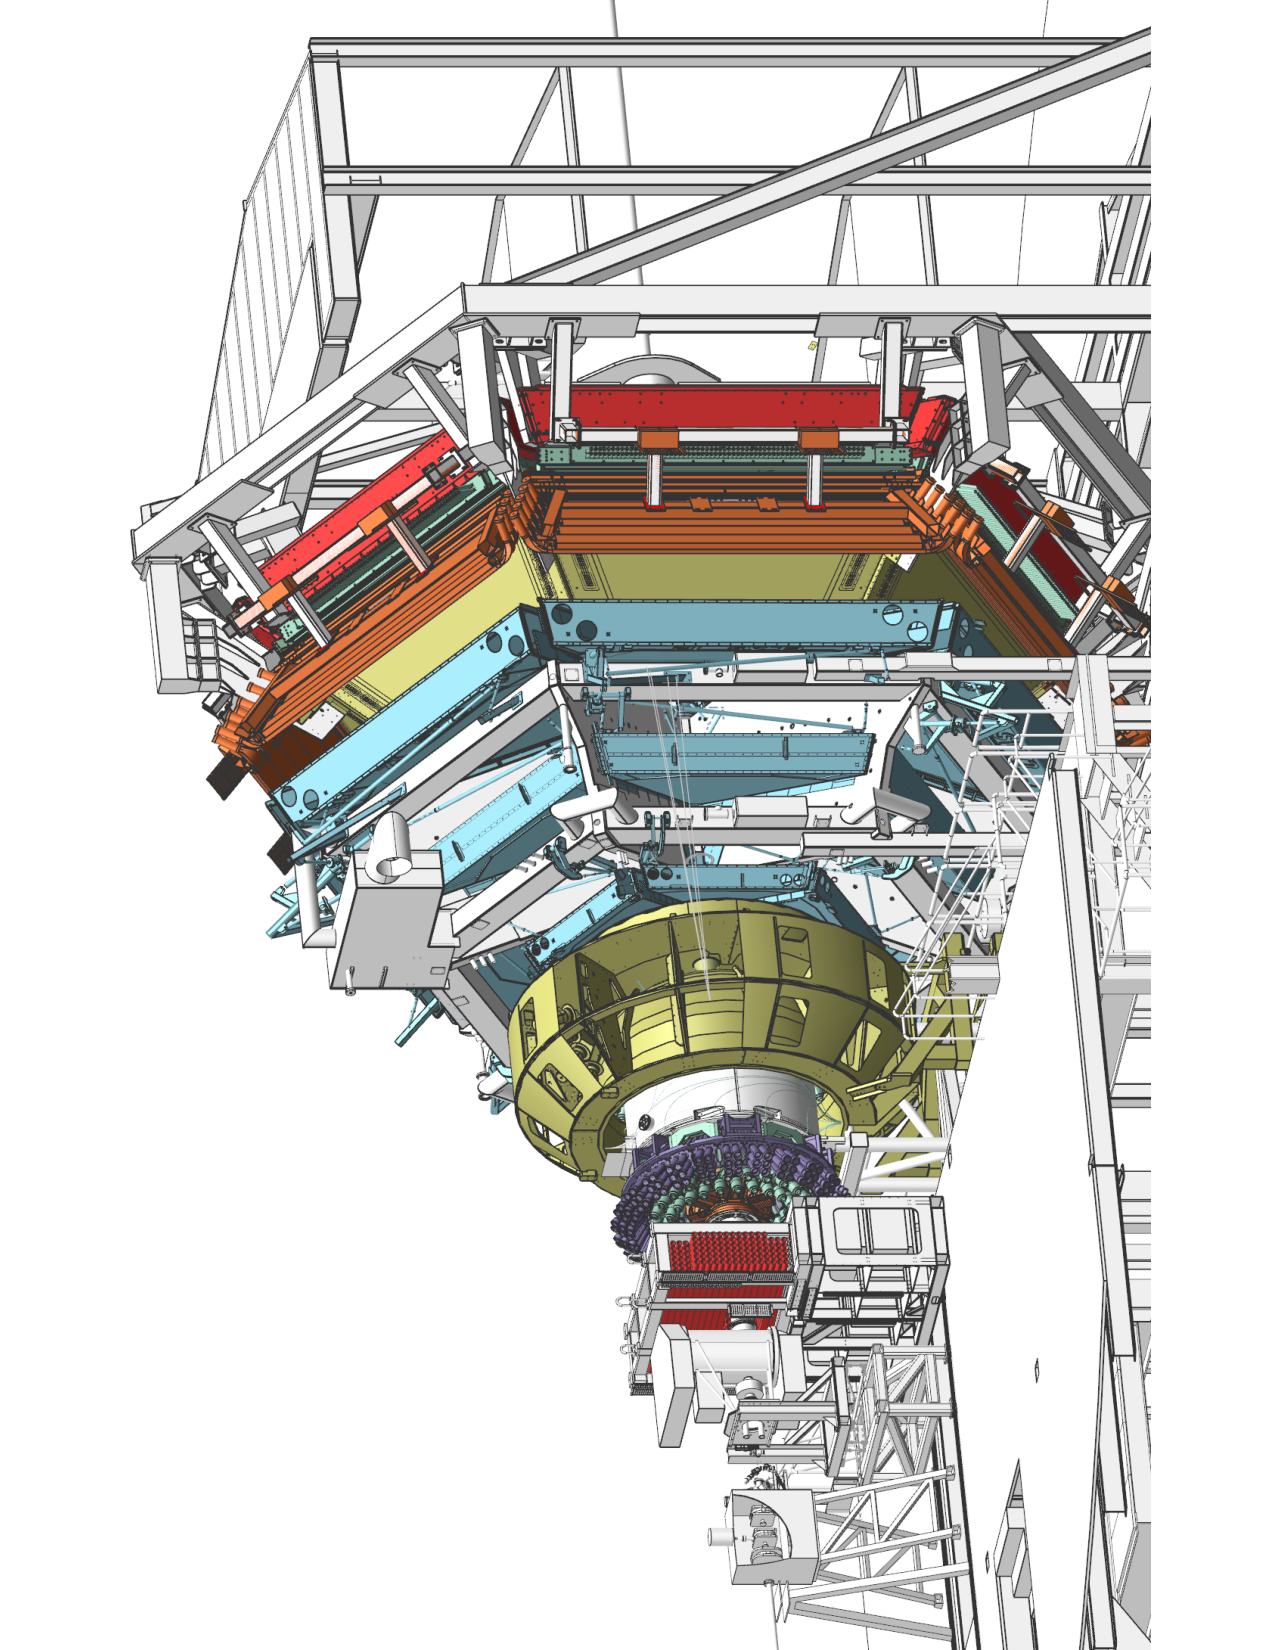
\includegraphics[width=0.70\textwidth,natwidth=610,natheight=642,angle=-90]{pics/ftof_clas12.pdf}}}
\end{picture} 
\caption{(Color Online) Model representation of the CLAS12 spectrometer in Hall~B at Jefferson Laboratory.
The electron beam is incident from the left side of this figure. The CLAS12 detector is roughly 10~m in
scale along the beam axis. For further details on the individual subsystems that make up the CLAS12
spectrometer see Ref.~\cite{clas12-nim}.}
\label{clas12-model}
\end{figure}
%%%%%%%%%%%%%%%%%%%%%%%%%%%%%%%%%%%%%%%%%%%%%%%%%%%%%%%%%

This paper focuses on the CLAS12 FTOF detector system and is organized as follows:
Section~\ref{clas12-fd-pid} reviews the scheme for particle identification in the CLAS12 Forward
Detector, Section~\ref{sec:overview} provides a high-level overview of the FTOF system and its
overall design requirements, Section~\ref{sec:design} provides a technical description of the system
design, and Section~\ref{sec:performance} highlights the performance of the system through both
bench testing with cosmic rays, as well as during the 2017 commissioning run and 2018 first production
run with electrons. Finally, Section~\ref{sec:summary} provides a summary of the FTOF system for
CLAS12.

\section{CLAS12 Forward Detector Particle Identification}
\label{clas12-fd-pid}

Particle identification in the CLAS12 Forward Detector relies on input from each of the different
forward detector subsystems. A reconstructed track in the Drift Chambers (DC) identifies the
presence of a charged particle and is used as a veto for forward-going neutral particles. The curvature
of the particle tracks in the magnetic field of the torus provides the electric charge. The other detector
subsystems are used to identify the particle type. These subsystems include the different Cherenkov
counters (HTCC, LTCC, and RICH), the electromagnetic calorimeters (ECAL), and the FTOF system.
These systems are used as part of the overall CLAS12 particle identification scheme to separate the
different particle species as a function of momentum.

CLAS12 consists of three different Cherenkov counters in the Forward Detector. A CO$_2$ filled
High Threshold Cherenkov Counter (HTCC) is positioned just downstream of the solenoid magnet. The
HTCC is used in conjunction with the electromagnetic calorimeters (ECAL) to identify scattered electrons
over their full momentum range. The HTCC threshold for pions is $\sim$5~GeV and is therefore used for
$e/\pi$ discrimination up to this threshold. The HTCC is also used for $\pi/K$ and $\pi/p$ separation
from $\sim$5-9~GeV. The $C_4F_{10}$ filled Low Threshold Cherenkov Counter (LTCC) is included in four
of the six CLAS12 sectors just upstream of the FTOF. This system is used for $\pi/K$ and $\pi/p$
separation for particle momenta in the range from $\sim$3-9~GeV. Finally, an aerogel-based Ring Imaging
Cherenkov (RICH) detector is included in one sector of CLAS12 and is used for $\pi/K$, $\pi/p$, and $K/p$
separation in the range of momenta from $\sim$3-8~GeV.

However, the primary system for particle identification in CLAS12 for forward-going charged particles
is the FTOF system. The main requirement for this system is that its counters provide excellent timing
resolution for particle identification. The FTOF  was designed to measure the flight time of charged
particles emerging from the target with an average timing resolution of 80~ps. Given this nominal timing
resolution for the counters, the momentum threshold for particle identification can be defined. For our
purposes, thresholds are quoted at the 4$\sigma$ level for FTOF, which amounts to the momenta where
particle identification can occur with up to an order of magnitude difference in the relative yields of the
different species. The timing resolution is illustrated by computing the flight time differences between
different charged particle species, pions, kaons, and protons, for tracks normally incident on the detector.
Fig.~\ref{tdiff} shows the computed time differences as a function of momentum. Where the 4$\sigma$
line crosses the computed time difference curves defines the momentum limit for particle identification
for each particle species. These limits are quoted as 2.8~GeV for $\pi/K$ separation, 4.8~GeV for $K/p$
separation, and 5.4~GeV for $\pi/p$ separation.  Fig.~\ref{clas12-pid} shows the different detector
subsystems used for charged particle identification of forward-going charged particles in CLAS12 and the
range of momenta for which they are responsible for the separation of the different particle species.

%%%%%%%%%%%%%%%%%%%%%%%%%%%%%%%%%%%%%%%%%%%%%%%%%%%%%%%%%
\begin{figure}[htbp]
\vspace{5.0cm}
\begin{picture}(50,50) 
\put(35,-105)
{\hbox{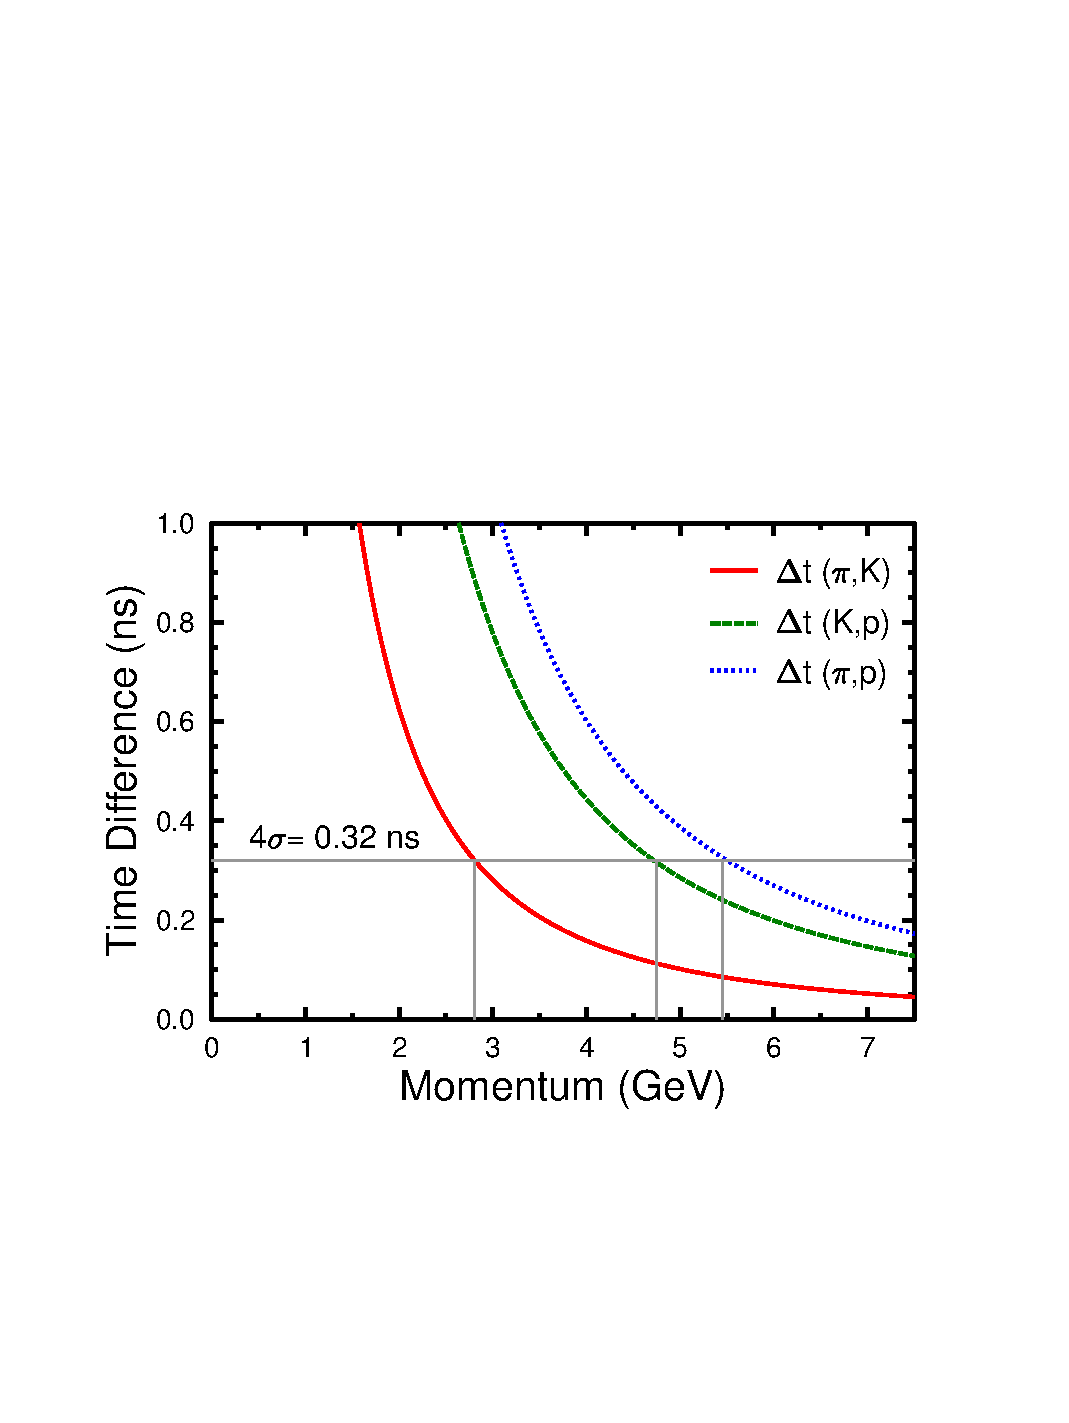
\includegraphics[width=1.0\textwidth,natwidth=610,natheight=642]{pics/tdiff_sep18.pdf}}}
\end{picture} 
\caption{(Color Online) Time differences, $\Delta t$, between protons and pions, between protons and kaons,
and between kaons and pions (as indicated) over the $\sim$6-7~m path length from the target to the FTOF
system.  The horizontal line indicates a time difference four times larger than the average FTOF counter
design resolution of $\sigma_{TOF} \approx$ 80~ps. The vertical line that meets each curve represent the
momentum where 4$\sigma$ particle species separation is quoted.}
\label{tdiff}
\end{figure}
%%%%%%%%%%%%%%%%%%%%%%%%%%%%%%%%%%%%%%%%%%%%%%%%%%%%%%%%%

%%%%%%%%%%%%%%%%%%%%%%%%%%%%%%%%%%%%%%%%%%%%%%%%%%%%%%%%%
\begin{figure}[htbp]
\vspace{6.0cm}
\begin{picture}(50,50) 
\put(25,-35)
{\hbox{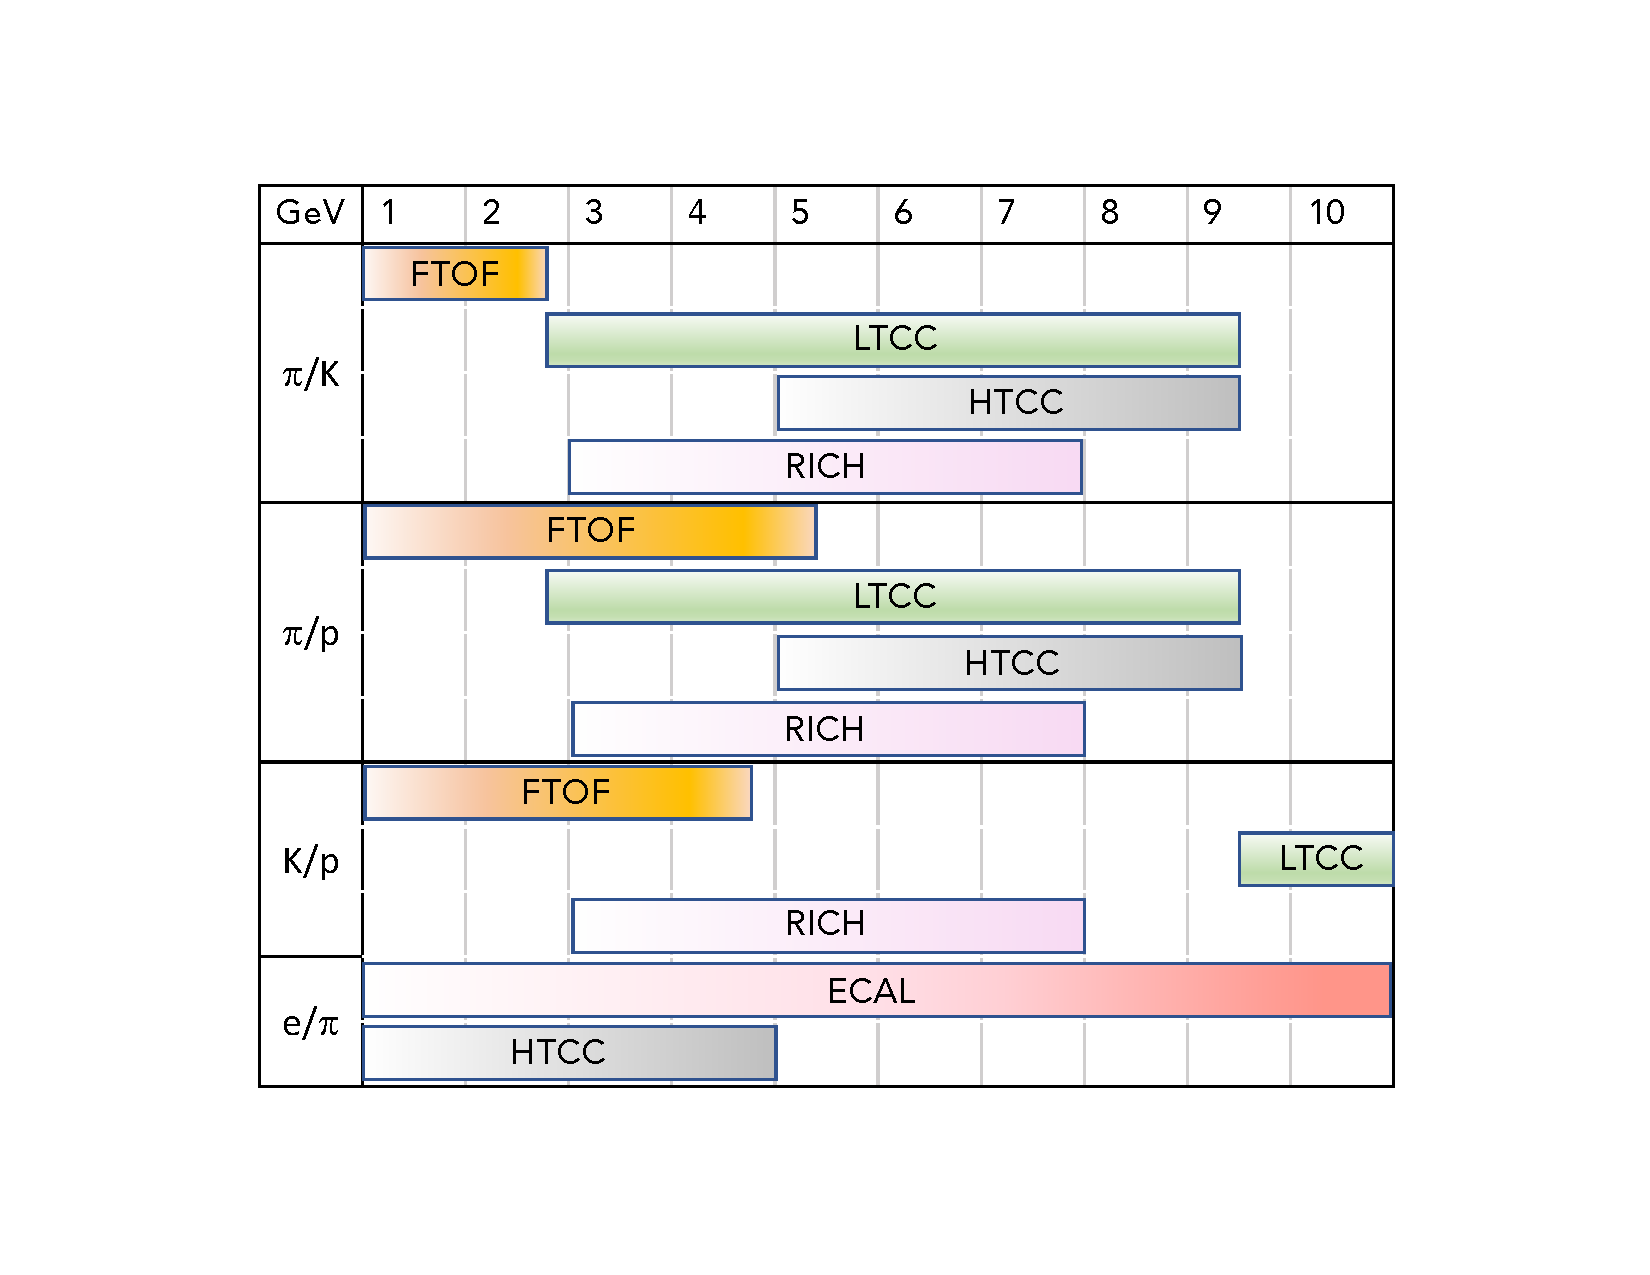
\includegraphics[width=0.70\textwidth,natwidth=610,natheight=642]{pics/clas12-pid-chart.pdf}}}
\end{picture} 
\caption{(Color Online) CLAS12 Forward Detector subsystems used for particle identification and the
range of momentum where they are effective in separating different particle species.}
\label{clas12-pid}
\end{figure}
%%%%%%%%%%%%%%%%%%%%%%%%%%%%%%%%%%%%%%%%%%%%%%%%%%%%%%%%%

Fig.~\ref{pth-kin} shows a plot of the momentum versus polar angle in CLAS12 from beam data of
an 11~GeV electron beam incident on a hydrogen target for a typical exclusive reaction
$ep \to e'K^+\Lambda$. For this reaction the typical charged hadron track momenta accepted by
FTOF are in the range from 1~GeV to 7~GeV.

%%%%%%%%%%%%%%%%%%%%%%%%%%%%%%%%%%%%%%%%%%%%%%%%%%%%%%%%%
\begin{figure}[htbp]
\vspace{5.0cm}
\begin{picture}(50,50) 
\put(-5,-55)
{\hbox{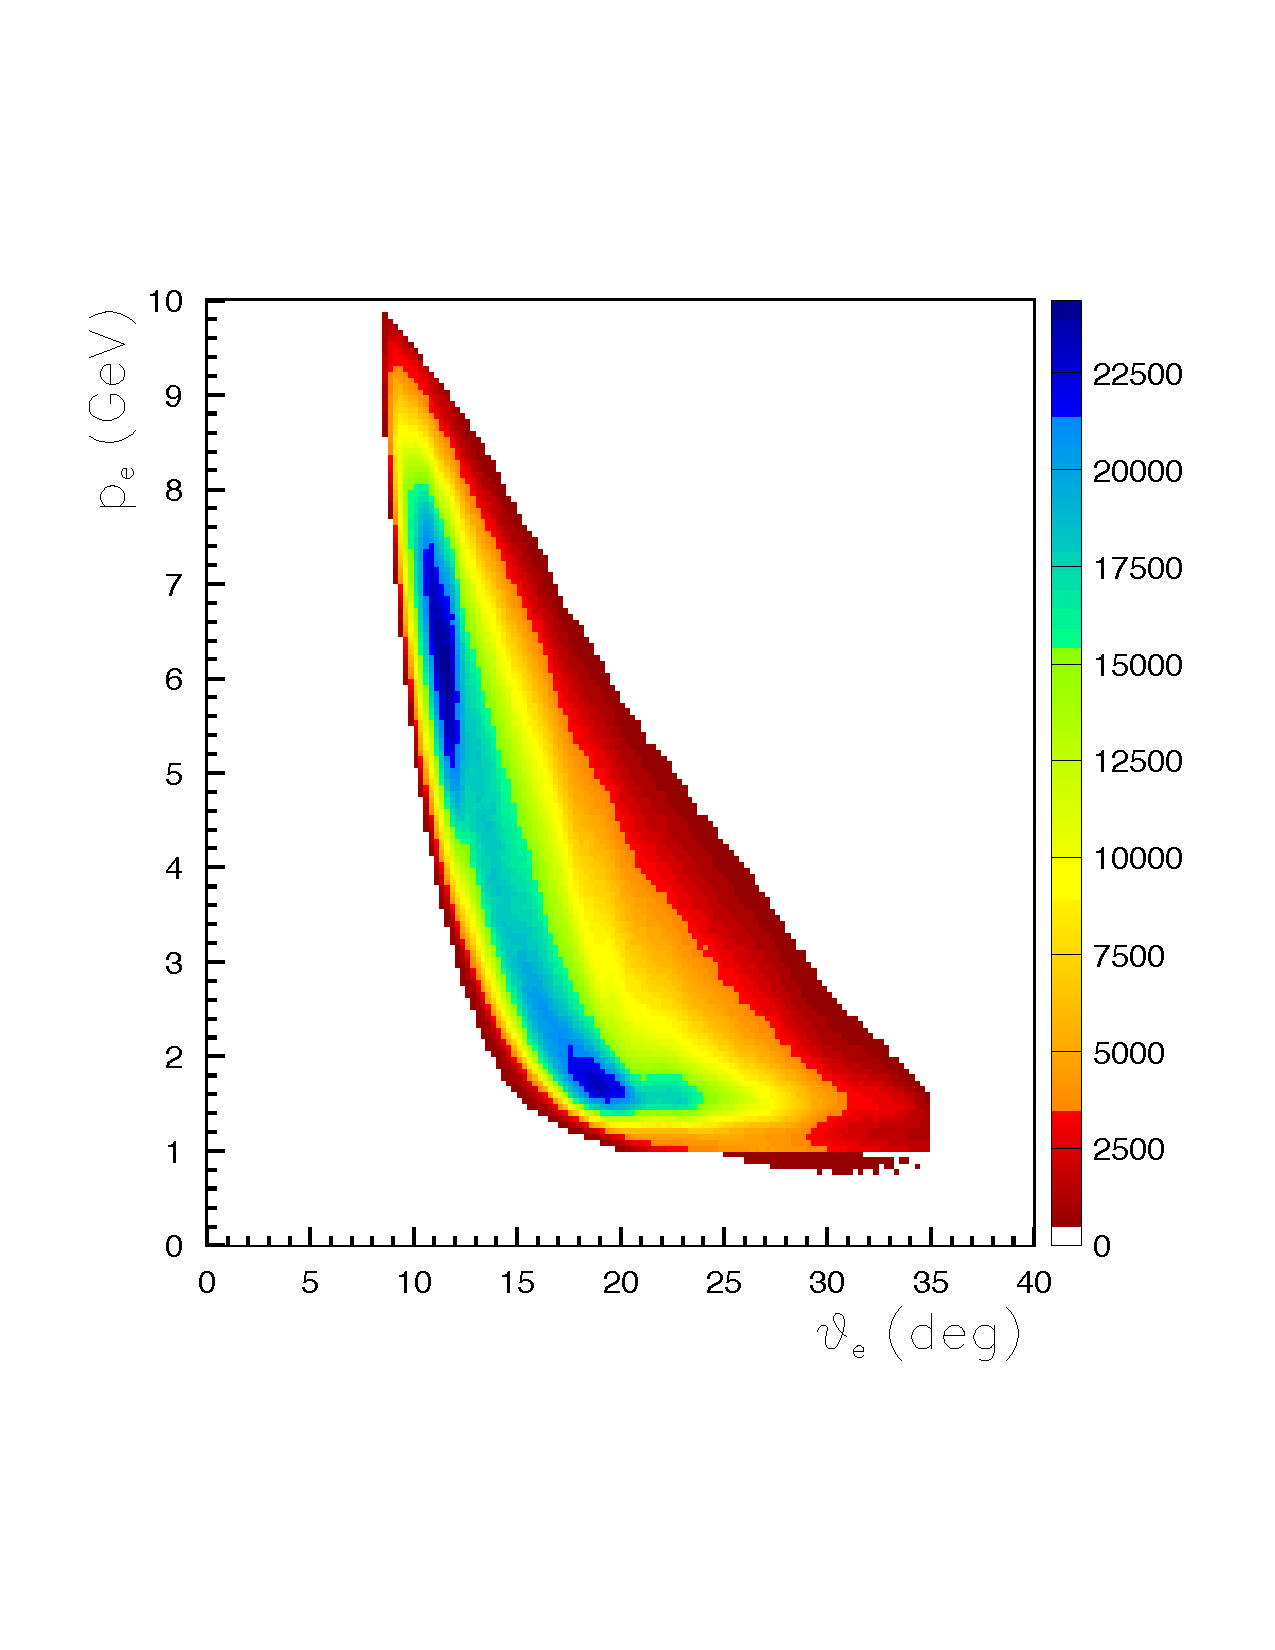
\includegraphics[width=0.55\textwidth,natwidth=610,natheight=642]{pics/pthe.pdf}}}
\put(190,-55)
{\hbox{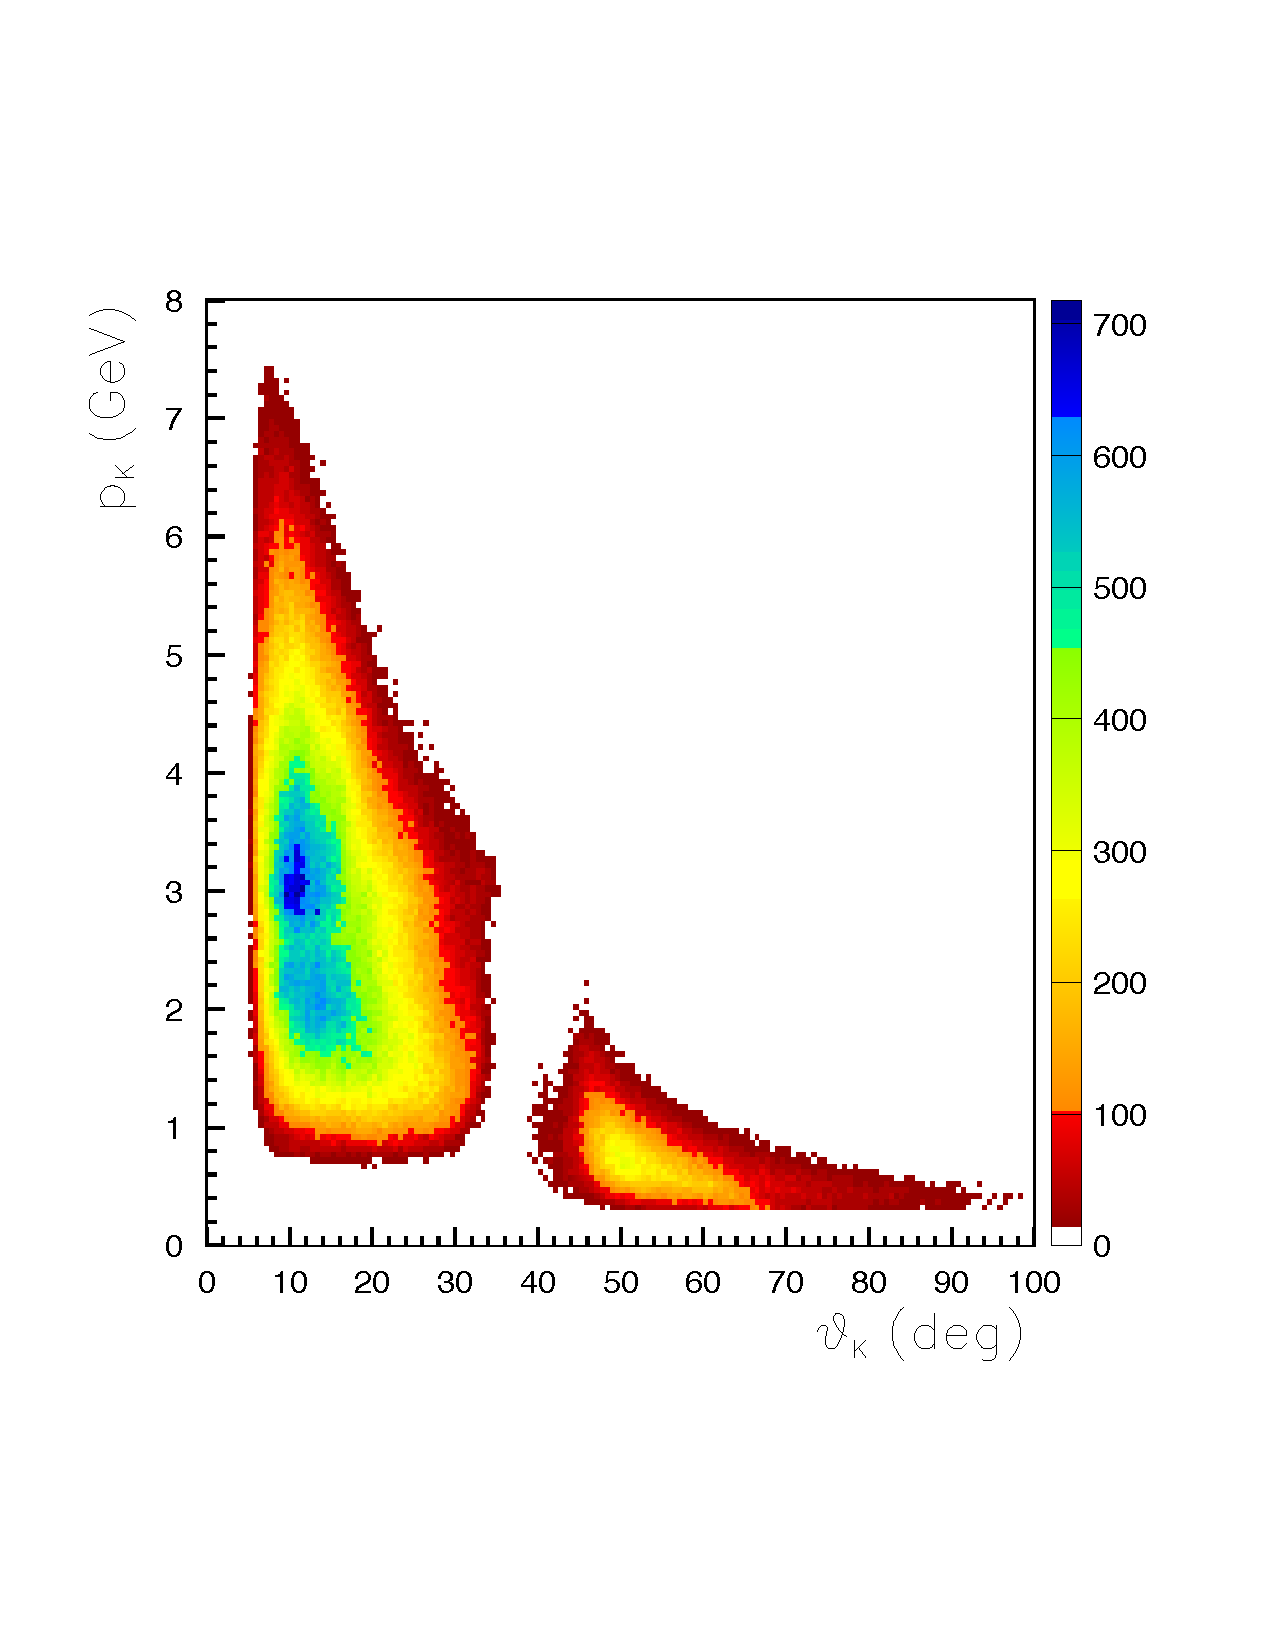
\includegraphics[width=0.55\textwidth,natwidth=610,natheight=642]{pics/pthkp.pdf}}}
\end{picture} 
\caption{(Color Online) Plot of momentum vs. angle from beam data for a 10.6~GeV electron beam incident
upon a liquid-hydrogen target in CLAS12 for selection of a final-state electron (left) and $K^+$ (right).
The discontinuity at $\theta=35^\circ$ is due to the small acceptance gap between the Forward and 
Central Detectors. The typical momentum of charged tracks in the Central Detector is less than 2~GeV.}
\label{pth-kin}
\end{figure}
%%%%%%%%%%%%%%%%%%%%%%%%%%%%%%%%%%%%%%%%%%%%%%%%%%%%%%%%%

\section{Overview of the FTOF System}
\label{sec:overview}

The Forward Time-of-Flight System (FTOF) is a major component of the CLAS12 Forward Detector
used to measure the time-of-flight of charged particles emerging from interactions in the target.
The requirements for FTOF include excellent timing resolution for charged particle identification and
good segmentation to minimize counting rates and to provide for flexible triggering options. The system
specifications call for an average time resolution of $\sigma_{TOF}$=80~ps at the more forward angles
of CLAS12 and 150~ps at angles larger than 35$^\circ$. The system must also be capable of operating in
a high-rate environment where the average counting rate for each FTOF scintillator at an operating
luminosity of $1 \times 10^{35}$~cm$^{-2}$s$^{-1}$ is $\sim$0.5-1~MHz.

In each of the six sectors of the CLAS12 Forward Detector, the FTOF system is comprised of three
arrays of counters, referred to as panels, named panel-1a, panel-1b, and panel-2. Each panel consists
of a set of rectangular scintillators with a photomultiplier tube (PMT) on each end. Panel-1 refers to
the counters located at forward angles (roughly 5$^\circ$ to 35$^\circ$) (where two panels are
employed to meet the 80~ps average time resolution requirement) and panel-2 refers to the sets of
counters at larger angles (roughly $35^\circ$ to 45$^\circ$). The positioning and attachment of the
FTOF detector arrays on their Forward Carriage supports are shown in Fig.~\ref{fwd_car}.

%%%%%%%%%%%%%%%%%%%%%%%%%%%%%%%%%%%%%%%%%%%%%%%%%%%%%%%%%
\begin{figure}[htbp]
\vspace{4.6cm}
\begin{picture}(50,50) 
\put(100,-35)
{\hbox{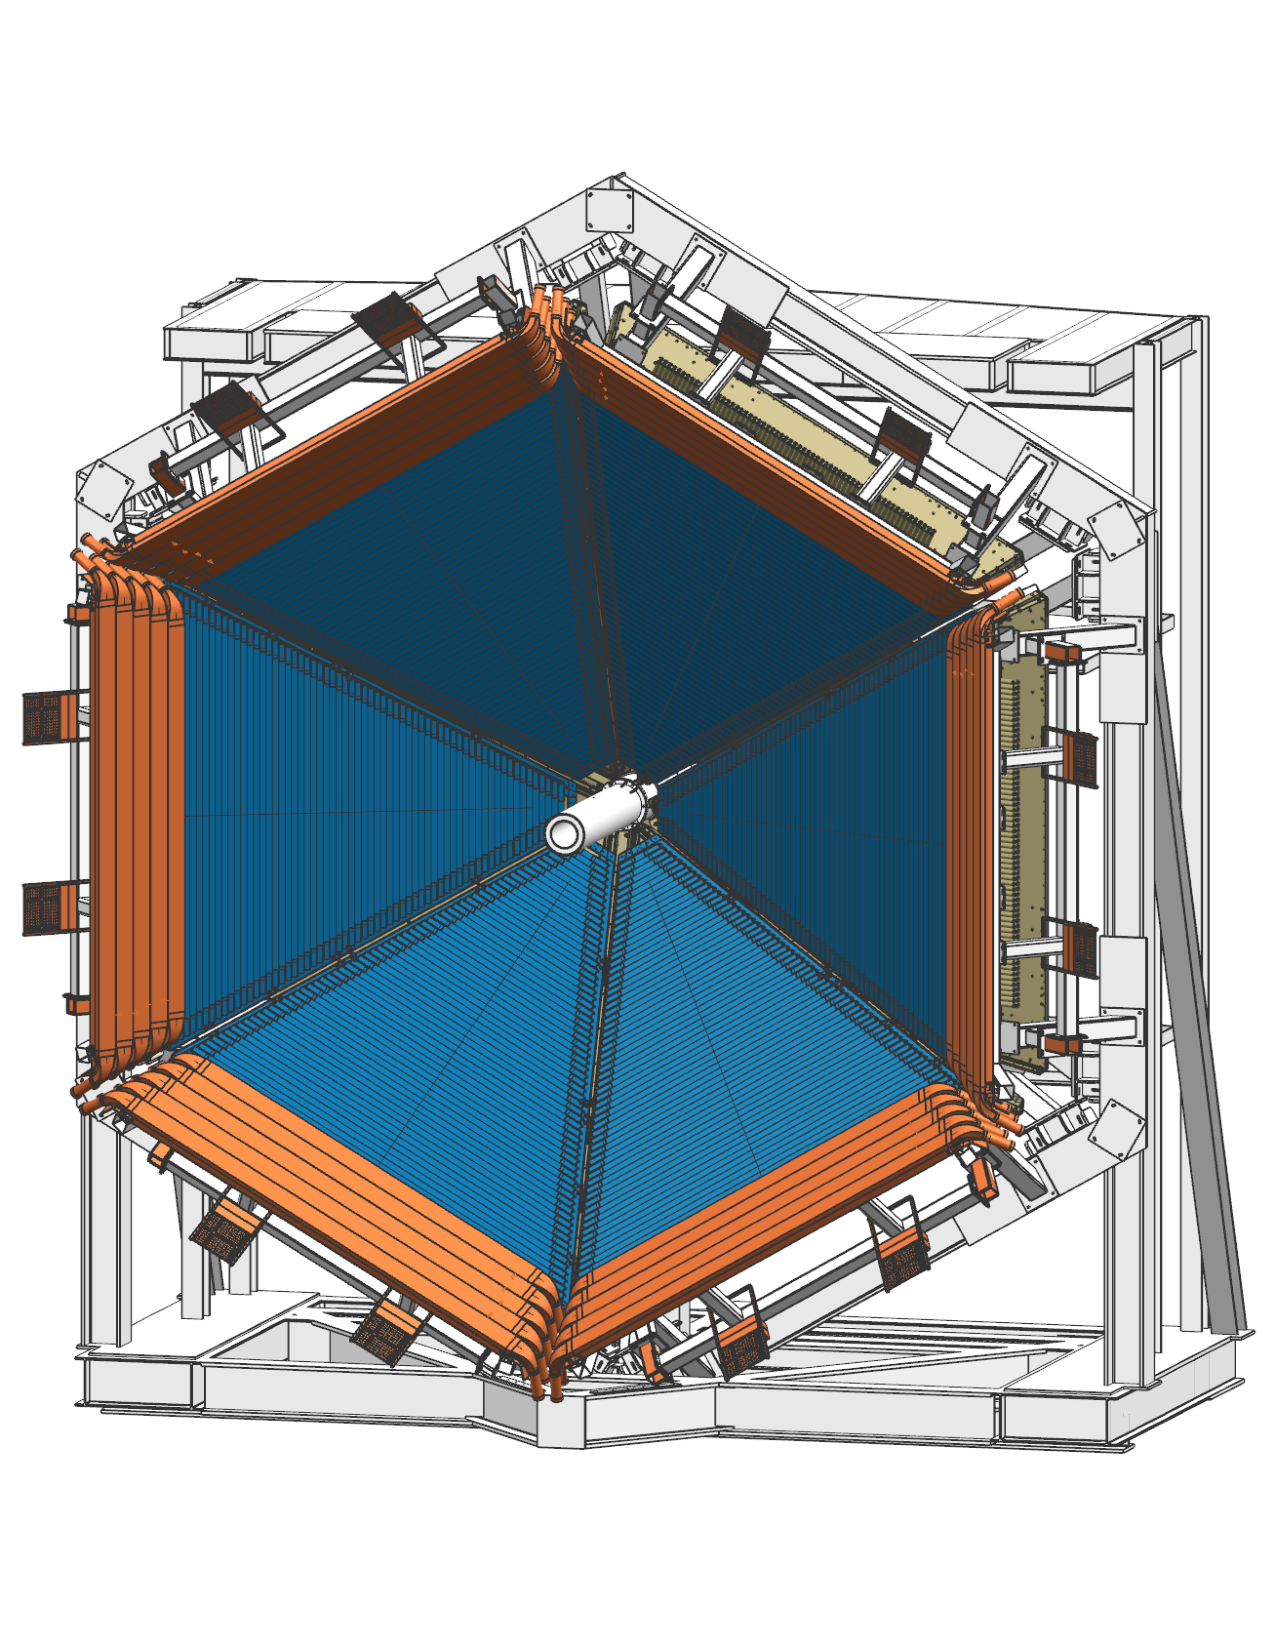
\includegraphics[width=0.50\textwidth,natwidth=610,natheight=642]{pics/fwd_carriage.pdf}}}
\end{picture} 
\caption{(Color Online) View of the FTOF counters for CLAS12 highlighting the location of the panel-1 and
panel-2 counters. The panel-1b counter arrays are shown in blue and the panel-2 counter arrays, mounted
around the perimeter of the Forward Carriage, are shown in orange. The panel-1a counter arrays mounted
just downstream of the panel-1b arrays are not visible in this picture. The Forward Carriage is roughly 10~m
in diameter.} 
\label{fwd_car}
\end{figure}
%%%%%%%%%%%%%%%%%%%%%%%%%%%%%%%%%%%%%%%%%%%%%%%%%%%%%%%%%

The FTOF counters in the angular range from 5$^\circ$ to 35$^\circ$ consist of two sets of six 
triangular arrays. Just upstream of the electromagnetic calorimeter (ECAL) detectors, the panel-1a arrays 
are mounted. These detector sets were refurbished from the panel-1 TOF counters from the decommissioned 
CLAS spectrometer~\cite{tof-nim}. Upstream of the panel-1a arrays the new panel-1b arrays are mounted. In
the event reconstruction the hit times for panel-1a and panel-1b are combined together to determine the
charged particle hit time (see Section~\ref{cluster}). In the angular range from 35$^\circ$ to 45$^\circ$ the
panel-2 arrays are mounted. These counters were refurbished from the panel-2 arrays of the CLAS TOF system.
A detailed summary of the FTOF technical parameters is given in Table~\ref{spec-table}. 

%%%%%%%%%%%%%%%%%%%%%%%%%%%%%%%%%%%%%%%%%%%%%%%%%%%%%%%%%
\begin{table}[t]
\begin{center}
\begin{tabular} {c|l} \hline
~~Parameter~~ &~~~~~~~~~~~~~~~~~~~~~~ Design Value ~~~~~~~~~~\\ \hline \hline
\multicolumn{2}{l} {\bf Panel-1a} \\ \hline
Angular Coverage      & $\theta = 5^\circ \to 35^\circ$, $\phi: 50\% {\rm ~at~} 5^\circ \to 85\% {\rm ~at~} 
35^\circ$ \\ \hline
Counter Dimensions   & $L = 32.3$~cm $\to$ 376.1~cm, $w \times h$ = 15~cm $\times$ 5~cm   \\ \hline
Scintillator Material & BC-408   \\ \hline
PMTs                         & EMI 9954A, Philips XP2262 \\ \hline
Design Resolution     & 90~ps $\to$ 160~ps   \\ \hline \hline
\multicolumn{2}{l} {\bf Panel-1b} \\ \hline
Angular Coverage      & $\theta = 5^\circ \to 35^\circ$, $\phi: 50\% {\rm ~at~} 5^\circ \to 85\% {\rm ~at~} 
35^\circ$ \\ \hline
Counter Dimensions   & $L = 17.3$~cm $\to$ 407.9~cm, $w \times h$ = 6~cm $\times$ 6~cm   \\ \hline
Scintillator Material & BC-404 (\#1 $\to$ \#31), BC-408 (\#32 $\to$ \#62)  \\ \hline
PMTs                         & Hamamatsu R9779 \\ \hline
Design Resolution     & 60~ps $\to$ 110~ps   \\ \hline \hline
\multicolumn{2}{l} {\bf Panel-2} \\ \hline
Angular Coverage      & $\theta = 35^\circ \to 45^\circ$, $\phi: 85\% {\rm ~at~} 35^\circ \to 95\% {\rm ~at~} 
45^\circ$ \\ \hline
Counter Dimensions   & $L = 371.3$~cm $\to$ 426.1~cm, $w \times h$ = 22~cm $\times$ 5~cm   \\ \hline
Scintillator Material & BC-408   \\ \hline
PMTs                         & Photonis XP4312B, EMI 4312KB \\ \hline
Design Resolution     & 145~ps $\to$ 160~ps   \\ \hline
\end{tabular}
\caption{Table of parameters for the scintillators, PMTs, and counters for the FTOF panel-1a, panel-1b, 
and panel-2 arrays.}
\label{spec-table}
\end{center}
\end{table}
%%%%%%%%%%%%%%%%%%%%%%%%%%%%%%%%%%%%%%%%%%%%%%%%%%%%%%%%%

The panel-1 arrays consist of the old CLAS panel-1 TOF counters (called panel-1a) and a new set of panel-1
counters (called panel-1b).  The panel-1a arrays consist of 23 scintillators, each measuring 5.08-cm thick
and 15-cm wide.  The lengths of these counters range from roughly 32~cm at the smallest scattering angles
to roughly 376~cm at the largest scattering angles.  The scintillators are constructed from Bicron~\cite{bicron}
BC-408 and are read out through short acrylic light guides to 2-in Thorn EMI-9954A PMTs.  The new panel-1b
arrays consist of 62 scintillators constructed from Bicron BC-404 scintillator for the shorter counters and
BC-408 for the longer counters, each 6-cm wide and 6-cm thick. The lengths of these counters range from
roughly 17~cm at the smallest scattering angles to roughly 408~cm at the largest scattering angles. The
scintillators are read out through Hamamatsu R9779 PMTs~\cite{hamamatsu} coupled directly to the
scintillation bars. This new panel is mounted to the Forward Carriage in front of the panel-1a counters. The
detailed design and bench testing results for these counters is described in detail in Ref.~\cite{nim-p1b}.

The panel-2 arrays consist of selected counters from the old CLAS panel-2 TOF counters, and include 5
22-cm wide, 5.08-cm thick scintillators in each sector.  The length of these counters ranges from roughly
370~cm to 440~cm.  These scintillators are constructed from Bicron BC-408 and are read out through curved
acrylic light guides to 3-in Philips XP4312B PMTs. These scintillators are included to give complete acceptance
for outbending charged particles incident upon the CLAS12 drift chambers.  

\section{FTOF System Design}
\label{sec:design}

In order to meet the performance and mechanical requirements for the FTOF system, the major
considerations in its design included the system geometry and areal coverage, the counter and system
timing resolutions, the system components, and the design and materials associated with its mechanical
support structure in the active area of the spectrometer. These system design elements are described
in the following subsections. In addition, this section also includes information on the readout electronics
and the high voltage system used for the FTOF.

\subsection{Geometry}
\label{ftof-geometry}

The projected space behind the coils of the CLAS12 torus as defined by straight lines projecting from
the center of the nominal target position radially outward and is referred to downstream of the torus as
its shadow region. This region is inactive and defines the space available for locating the light guides,
photomultiplier tubes (PMTs), voltage dividers, and signal and high voltage cables. The remaining area in
the forward direction is the sensitive fiducial region of the detector and must be covered with scintillation
counters. The design specification for FTOF called for a minimum of 50\% azimuthal acceptance at 5$^\circ$
increasing to 95\% at 45$^\circ$.

%%%%%%%%%%%%%%%%%%%%%%%%%%%%%%%%%%%%%%%%%%%%%%%%%%%%%%%%%
\begin{figure}[htbp]
\vspace{4.7cm}
\begin{picture}(50,50) 
\put(0,-25)
{\hbox{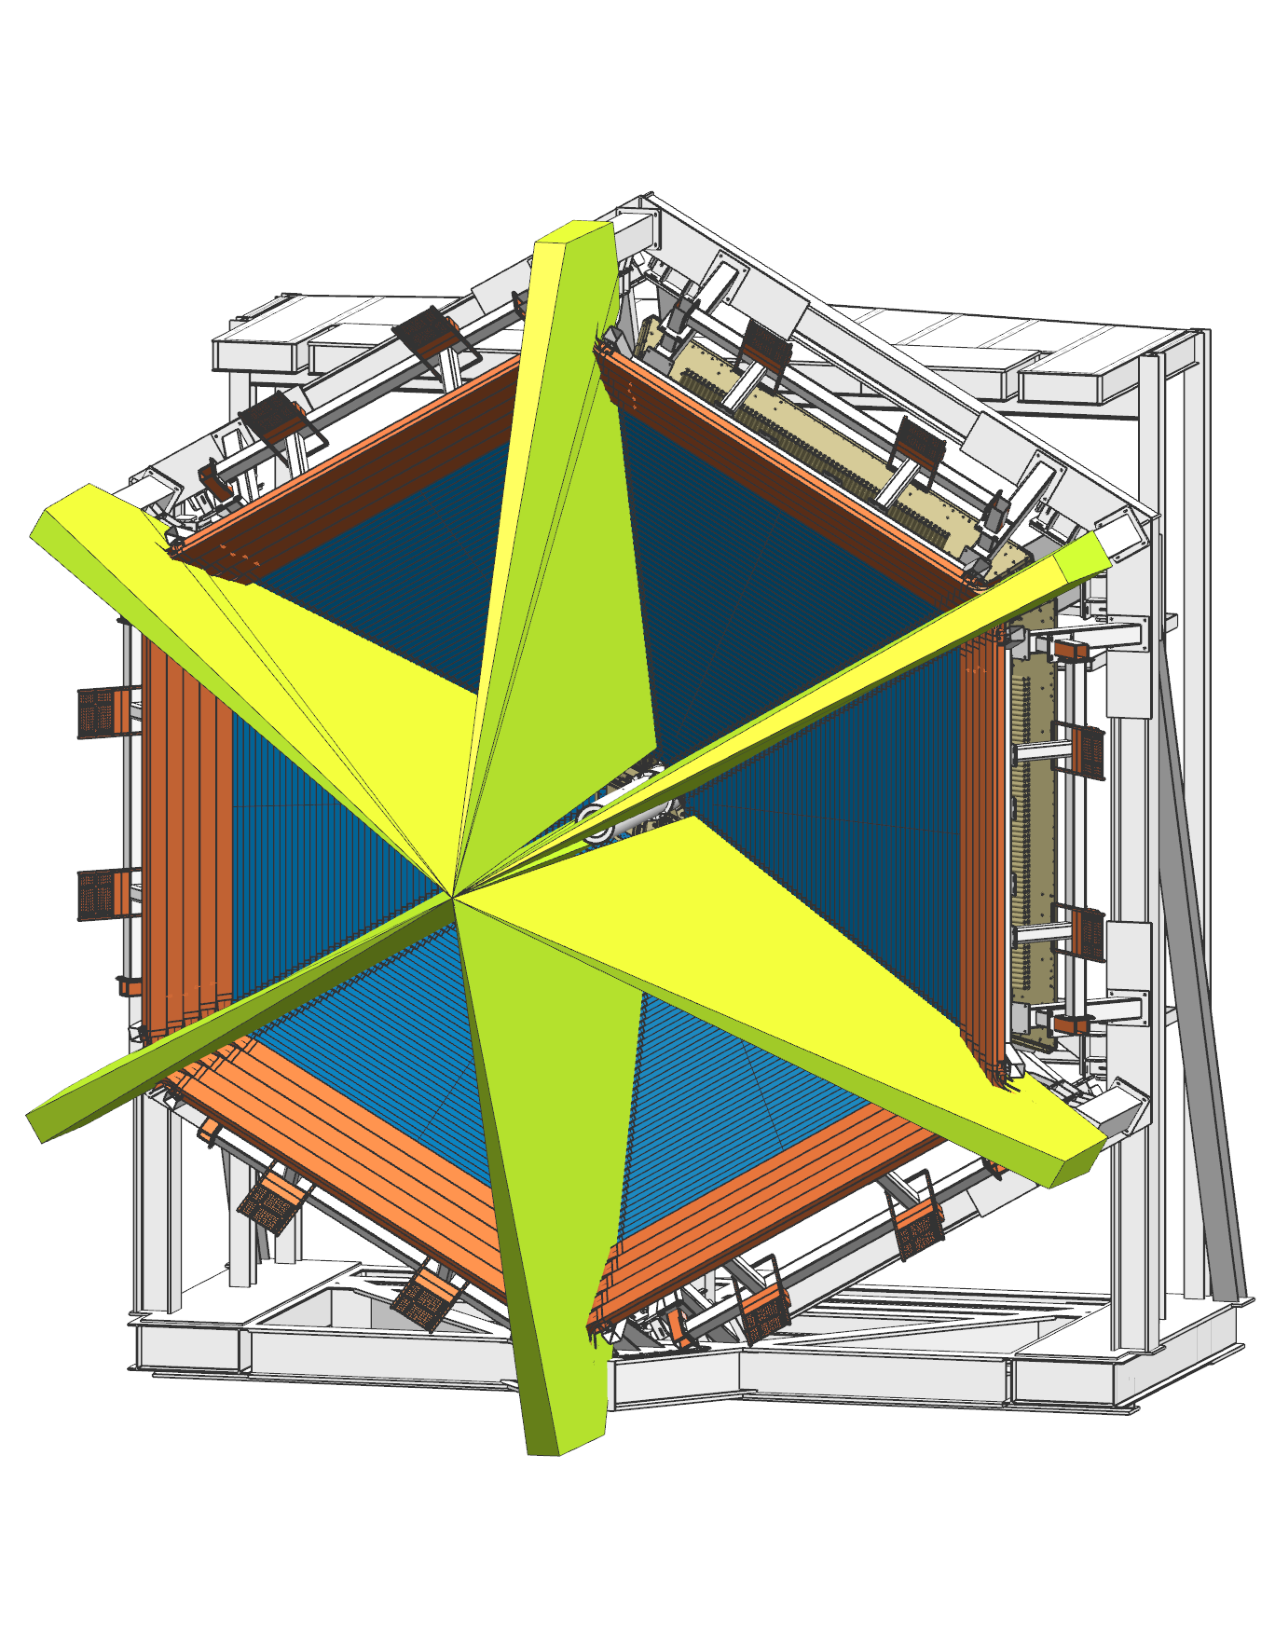
\includegraphics[width=0.45\textwidth,natwidth=610,natheight=642]{pics/fwd_shadow1.pdf}}}
\put(180,180)
{\hbox{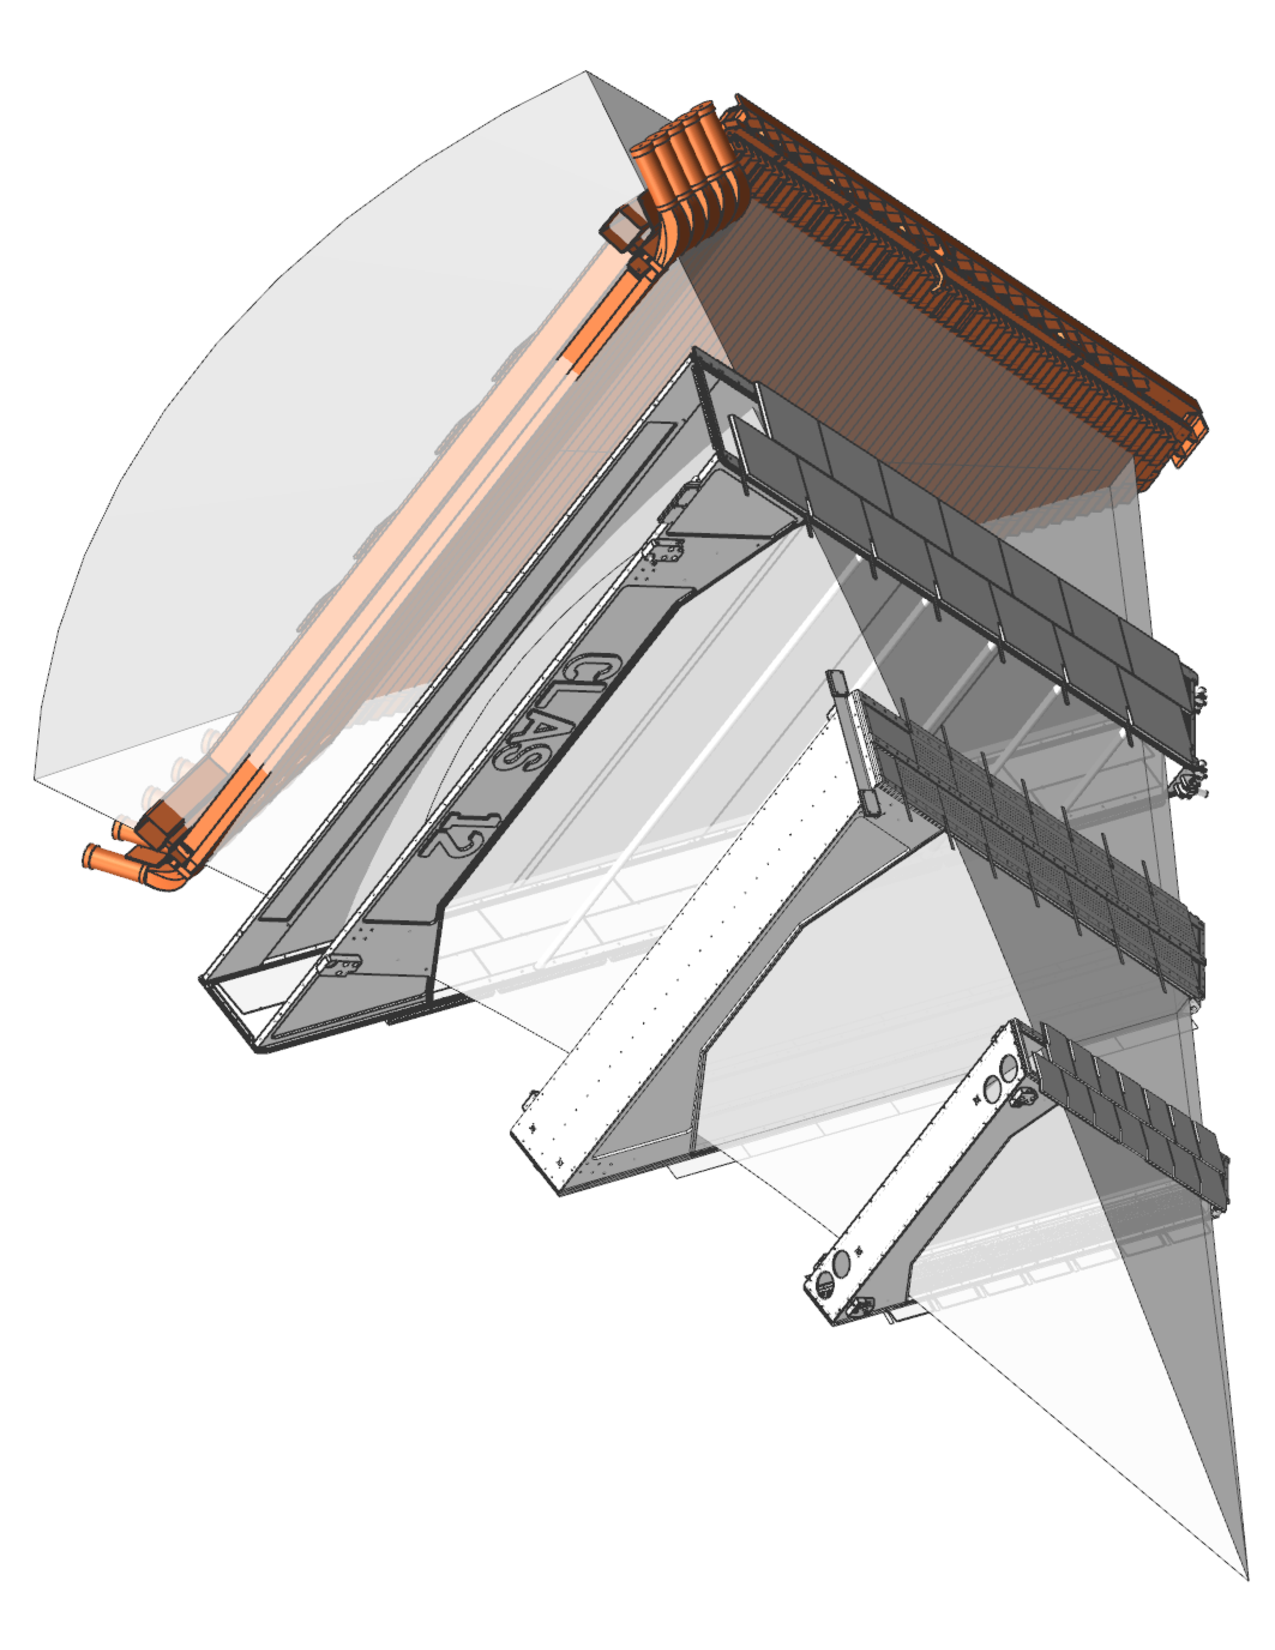
\includegraphics[width=0.45\textwidth,natwidth=610,natheight=642,angle=-90]{pics/fwd_shadow2.pdf}}}
\end{picture} 
\caption{(Color Online) (Left) View of the shadows created by the main torus cryostats and drift
chamber endplates as projected on the face of the FTOF system.  (Right) The defined active area
between the shadow projections through the three regions of drift chambers projected on the face
of the FTOF in a representative Forward Carriage sector.}
\label{shadow}
\end{figure}
%%%%%%%%%%%%%%%%%%%%%%%%%%%%%%%%%%%%%%%%%%%%%%%%%%%%%%%%%

Fig.~\ref{shadow} provides an illustration of the shadow region projected onto the Forward Carriage
created primarily by the torus cryostats and the drift chamber endplates as projected on the face of
the FTOF system. These pictures come from the CAD design model of CLAS12. Fig.~\ref{shadow}(left)
shows a picture of the shadow bands on the Forward Carriage that defines a uniform gap of $\sim$40~cm
between each sector. Fig.~\ref{shadow}(right) shows the defined active region in one sector of CLAS12 on
the face of the FTOF. The width of this area in azimuth at the position of the Forward Carriage in Hall~B
essentially defined the length of the scintillation counters. The final limits of the shadow region at the
location of FTOF are actually defined by the Region~2 Drift Chamber system.  While the Region~1 and
Region~3 chambers have their endplates, on-board electronics, and readout cables located mainly in the
shadow of the torus cryostats, the Region~2 chambers are located fully between the cryostats.

The panel-1a and panel-1b FTOF arrays in each sector are triangular in shape with the shortest counters
located closest to the beamline and the longest counters furthest from the beamline. The length of each
counter for a given counter number $N_{counter}$ is as follows:

\begin{itemize}
\item Panel-1a: $L (cm) = 15.85 \times N_{counter} + 16.43$ ~~($N_{counter} = 1 \to 5$), 
\item Panel-1a: $L (cm) = 15.85 \times N_{counter} + 11.45$ ~~($N_{counter} = 6 \to 23$), 
\item Panel-1b: $L (cm) = 6.40 \times N_{counter} + 10.84$ ~~($N_{counter} = 1 \to 62$).
\end{itemize}

The panel-1a and panel-1b arrays are tilted toward the target at an angle of 25$^{\circ}$ consistent with
the other subsystems in the CLAS12 Forward Detector (DC, LTCC, RICH, ECAL). The panel-1a counters
are located at a radial distance of the target in the range from $R$=724.21~cm for $N_{counter} = 1$ to
$R$=691.74~cm for $N_{counter} =23$. The panel-1b counters are located at a radial distance from the
target in the range from $R$=716.15~cm for $N_{counter} = 1$ to $R$=677.97~cm for $N_{counter}=62$.
The gap between the coplanar panel-1b and panel-1a arrays in each sector is 10.72~cm. The minimum angle
covered by panel-1a based on a straight line from the target is 5.453$^\circ$. The corresponding minimum
angle covered by panel-1b is 3.667$^\circ$. Each of the panel-1a arrays covers an area of 7.0~m$^2$ and
each of the panel-1b arrays covers an area of 7.9~m$^2$. Fig.~\ref{side-view} shows a two-dimensional
schematic of the layout and positioning of the arrays defining the key geometry parameters, which are
listed in Table~\ref{geom-parms}. See Ref.~\cite{ftof-geom} for more information.

The panel-2 arrays are mounted radially outward of the panel-1a and panel-1b arrays as shown in
Fig.~\ref{side-view}. The length of each counter for a given counter number $N_{counter}$ is as follows:

\begin{itemize}
\item Panel-2: $L (cm) = 13.73 \times N_{counter} + 357.55$~~ ~~($N_{counter} = 1 \to 5$).
\end{itemize}

The panel-2 arrays are tilted toward the target at an angle of 58.11$^\circ$. The minimum angle covered
by panel-2 based on a straight line from the target is 34.698$^\circ$. Each of the six panel-2 arrays
covers an area of 4.4~m$^2$. Note that the panel-2 arrays are not visible in the CLAS12 acceptance as
seen by straight lines from the center of the target. However, due to the presence of the toroidal magnetic
field, they provide additional acceptance for low momentum tracks  and for tracks associated with strange
particles that decay in-flight after emerging from the target (e.g. $\Lambda \to N \pi$ with $c \tau = 7.89$~cm).

%%%%%%%%%%%%%%%%%%%%%%%%%%%%%%%%%%%%%%%%%%%%%%%%%%%%%%%%%
\begin{figure}[htbp]
\vspace{5.5cm}
\begin{picture}(30,50) 
\put(0,-50)
{\hbox{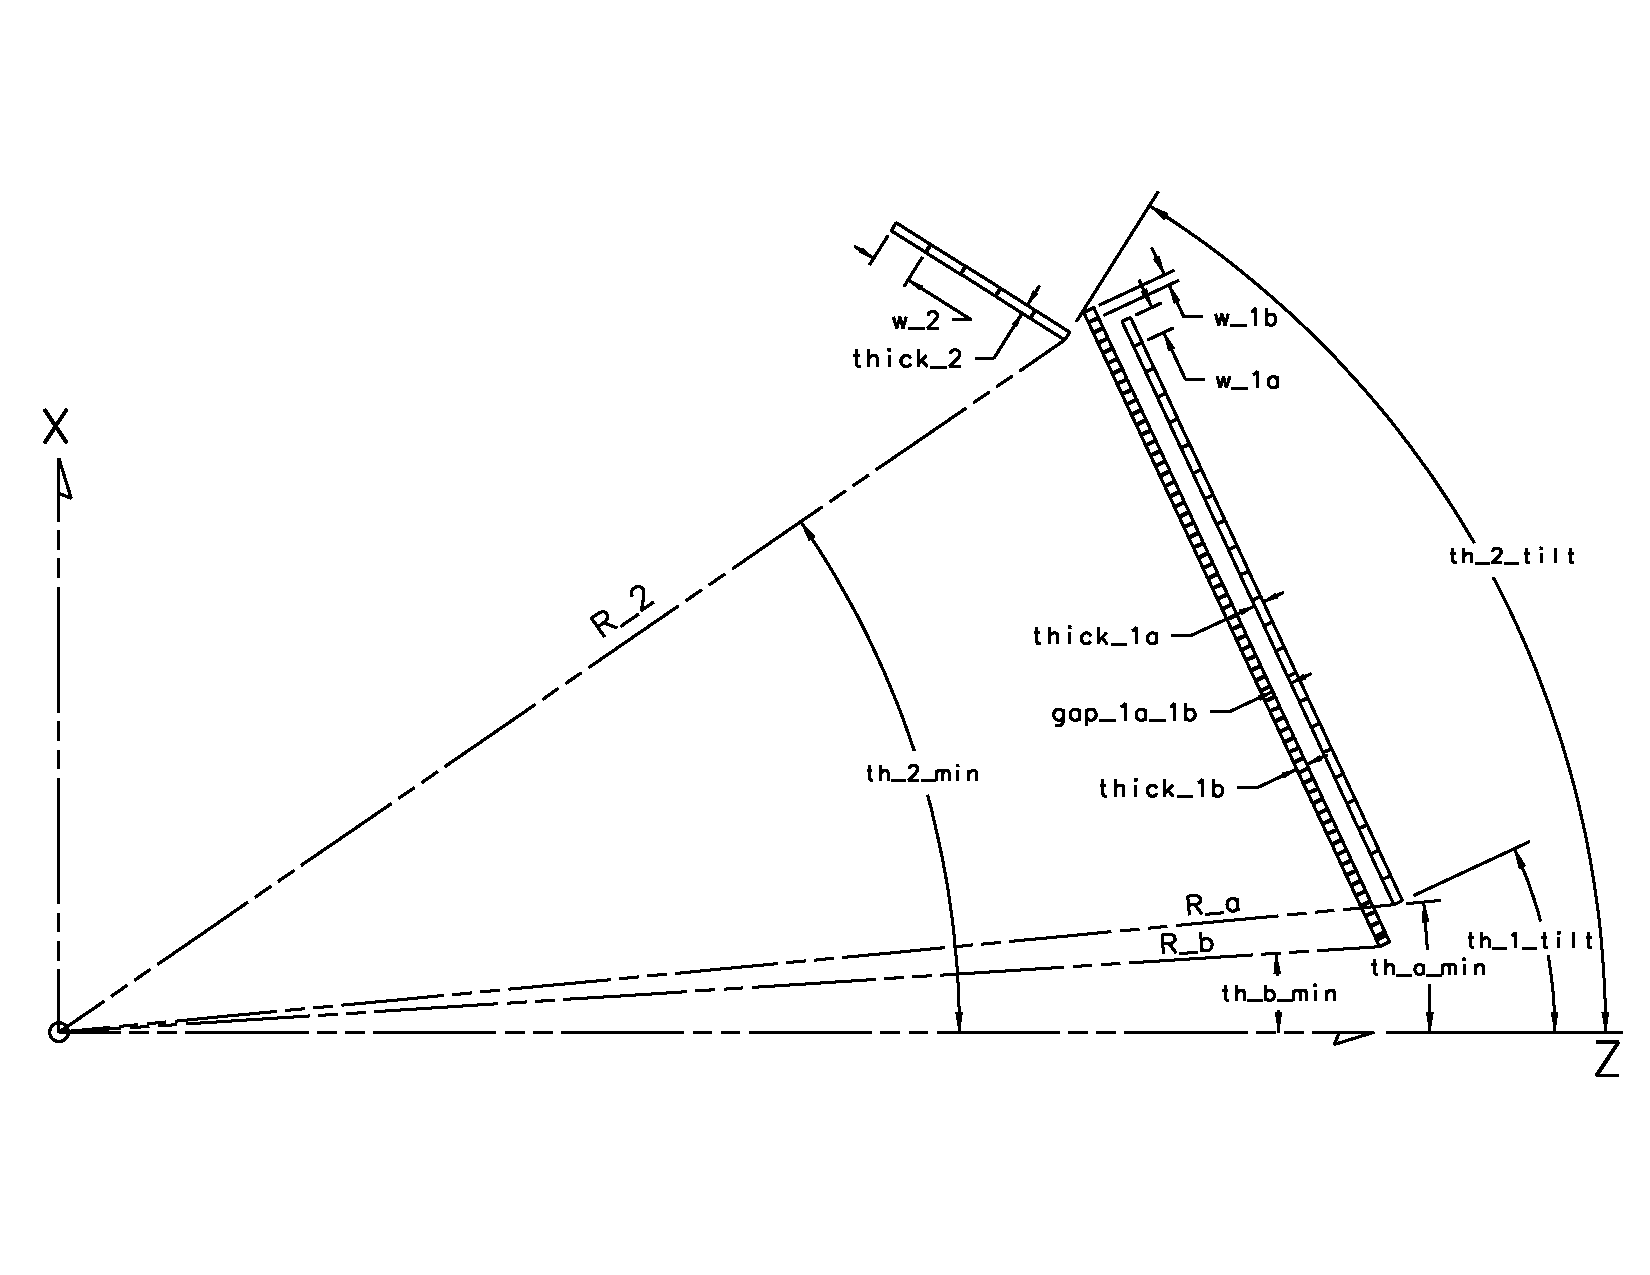
\includegraphics[width=0.75\textwidth,natwidth=610,natheight=642]{pics/side-view.pdf}}}
\end{picture} 
\caption{View of the FTOF scintillators for panel-1a, panel-1b, and panel-2 in the sector mid-plane for one
representative sector of the CLAS12 Forward Detector with the key parameters indicated.}
\label{side-view}
\end{figure}
%%%%%%%%%%%%%%%%%%%%%%%%%%%%%%%%%%%%%%%%%%%%%%%%%%%%%%%%%

%%%%%%%%%%%%%%%%%%%%%%%%%%%%%%%%%%%%%%%%%%%%%%%%%%%%%%%%%
\begin{table}[htbp]
\begin{center}
\begin{tabular} {c|c|c|c} \hline
Parameter & \multicolumn{3}{c}{Nominal Value}\\ \hline
R                & 726.689~cm & 717.236~cm & 659.71~cm\\ \hline
th\_min    & 5.453$^\circ$ & 3.667$^\circ$ & 34.698$^\circ$ \\ \hline
th\_tilt    & 25.00$^\circ$ & 25.00$^\circ$ & 58.11$^\circ$ \\ \hline
thick        & 5.08~cm           & 6.00~cm         & 5.08~cm \\ \hline
width       & 15.00~cm         & 6.00~cm         & 22.00~cm \\ \hline
gap\_1a\_1b & \multicolumn{2}{c|}{10.717~cm} &  -- \\ \hline
\end{tabular}
\caption{Table of the nominal geometry parameters for the CLAS12 FTOF detector system.}
\label{geom-parms}
\end{center}
\end{table}
%%%%%%%%%%%%%%%%%%%%%%%%%%%%%%%%%%%%%%%%%%%%%%%%%%%%%%%%%%

Given the active area coverage requirements for the FTOF system within each CLAS12 sector on the
Forward Carriage, another key aspect of the geometry associated with the FTOF system design is
the width of the individual scintillation counters. An essential optimization was made to select the
counter width to reduce the number of readout channels while considering the overall counting rates per
bar at the nominal luminosity associated with incident charged and neutral particles including photons.
These rates must allow for reasonable PMT anode currents that do not affect the stability of the PMT
response in terms of pulse shape or saturation effects, or lead to unreasonably short PMT lifetimes
defined in terms of the total integrated charge collected at the first dynode of the PMT. In addition, the
width of the scintillation bars determines the granularity of the scattering angle definition in the trigger
and its matching to the projected tracks from the Drift Chambers and toward the electromagnetic
calorimeters. Note that the 15~cm widths of panel-1a and the 22~cm widths of panel-2 from the existing
refurbished counters from the CLAS TOF system were optimized for nominal beam-target luminosities a
factor of 10 lower than for CLAS12. The 6~cm widths of the newly constructed panel-1b counters were
optimized for the higher rate operating conditions of CLAS12.

\subsection{Time Resolution}
\label{res-sec}

Time-of-flight detectors are designed to provide an output signal for the data acquisition system that
reflects the time a charged particle passed through the scintillation counter. As the particle passes
through the scintillation material, it causes ionization that subsequently generates scintillation light. The
photons that are created travel on various paths inside of the scintillator and light guide (if present), which
may get absorbed, reflected (internally or on outer wrapping materials), and ultimately impinge on the
photocathode of the PMT. This interaction produces a photoelectron signal that is amplified within the stages
of the PMT and this pulse is then input into the readout electronics, which includes a discriminator and a
time-to-digital (TDC) converter. The net effect of these different processes accounts for the time resolution
of the counter $\sigma_{TOF}$.

The contributions to the time resolution of TOF systems have been parameterized in Ref.~\cite{kuhlen}
using the following form:

\begin{equation}
\label{timing-func}
\sigma_{TOF} = \sqrt{\sigma_0^2 + \frac{\sigma_1^2 + (\sigma_2 L/2)^2} {N_{pe}}}.
\end{equation}

Here $\sigma_0$ represents the intrinsic electronic resolution of the measurement system. This represents
a floor-term contribution that is independent of light level. The remaining terms $\sigma_1$ and $\sigma_2$
are directly dependent on the photo-statistics at the PMT photocathode $N_{pe}$. The term $\sigma_1$
models the jitter in the combined single photoelectron response of the scintillation counter and its PMTs and
the term $\sigma_2$ accounts for path length variations in the light collection.  These path length variations
in the scintillator scale with the distance from the source to the PMT, which we take to be half the length of
the counter ($L/2$), since the scintillators are read out at either side.  The statistical behavior of the last
two terms is indicated by scaling the single-photoelectron responses by $\sqrt{N_{pe}}$, where $N_{pe}$ is
the average number of photoelectrons seen by the PMT of a counter with an infinitely long attenuation length.
For scintillators that are several meters long, the dominant contribution comes from transit time variations of
photon paths in the scintillator.

The values of the parameters $\sigma_0$, $\sigma_1$, and $\sigma_2$ for the panel-1a and panel-2 counters
are given in the CLAS TOF paper~\cite{tof-nim}, where the above functional form with the parameters listed
in Table~\ref{timing-parms} was found to well describe the measured data. A direct extension of these
parameters is assumed to be reasonable for estimating the timing resolution for the panel-1b counters. For the
estimates used for the FTOF timing resolutions, the parameters employed are listed in Table~\ref{timing-parms}.
Note that due to improvements in the resolution of the readout electronics for the CLAS12 FTOF system compared
to the CLAS TOF system, the floor-term $\sigma_0$ has been reduced from 62~ps to 40~ps. 

%%%%%%%%%%%%%%%%%%%%%%%%%%%%%%%%%%%%%%%%%%%%%%%%%%%%%%%%%
\begin{table}[htbp]
\begin{center}
\begin{tabular} {c|c} \hline
Parameter    & Nominal Value\\ \hline
$\sigma_0$ & 0.062~ns [CLAS TOF]; 0.040~ns [CLAS12 FTOF] \\ \hline
$\sigma_1$  & 2.1~ns [panel-1a/1b]; 2.0~ns [panel-2] \\ \hline
$\sigma_2$  & 2.0~ns \\ \hline
$N_{pe}^0$   & 918 \\ \hline
$\lambda$   & $0.358\cdot L + 81.725$~cm \\ \hline
\end{tabular}
\caption{Parameters determined for the CLAS TOF panel-1a and panel-2 counters in Ref.~\cite{tof-nim}
and used for a parameterization of the CLAS12 FTOF counters using the functional form for $\sigma_{TOF}$
in Eq.(\ref{timing-func}) and for $N_{pe}$ in Eq.(\ref{nphe-eq}).}
\label{timing-parms}
\end{center}
\end{table}
%%%%%%%%%%%%%%%%%%%%%%%%%%%%%%%%%%%%%%%%%%%%%%%%%%%%%%%%%%

The number of photoelectrons $N_{pe}$ in Eq.(\ref{timing-func}) for panel-1a and panel-2 at the PMT
photocathode was determined in Ref.~\cite{tof-nim} according to:

\begin{equation}
\label{nphe-eq}
N_{pe} = N_{pe}^0 {\rm exp} \left( \frac{L_0}{2 \lambda_0} - \frac{L}{2 \lambda} \right) \cdot F,
\end{equation}

\noindent
where $N_{pe}$ for all counters was referenced to the average value measured for the response of the
shortest panel-1a counter $N_{pe}^0$ of length $L_0=32$~cm with attenuation length $\lambda_0$. For the
panel-2 counters, $N_{pe}$ is further scaled by the factor $F = 0.9$ to account for light collection
efficiencies at the end of the larger panel-2 counters with their 3-in PMTs and longer light guides compared
to the smaller panel-1a PMTs with their relatively short light guides~\cite{tof-nim}. For the panel-1b counters,
$N_{pe}$ is determined as for panel-1a using Eq.(\ref{nphe-eq}) by scaling by the ratio of the widths of the
cross sectional areas of the scintillation bars (15~cm x 5~cm vs. 6~cm x 6~cm). 

Fig.~\ref{sigma_tof} shows the parameterized resolution for the counters in panel-1a, panel-1b, and panel-2
as a function of counter length. The Forward Detector event reconstruction and particle identification uses
timing information from both panel-1a and panel-1b. For tracks that pass through both arrays the combined
timing information (described in Section~\ref{cluster}) is used and results in a 20\% improvement compared to
using the hit information from panel-1b alone.

%%%%%%%%%%%%%%%%%%%%%%%%%%%%%%%%%%%%%%%%%%%%%%%%%%%%%%%%%
\begin{figure}[htbp]
\vspace{4.4cm}
\begin{picture}(50,50) 
\put(25,-55)
{\hbox{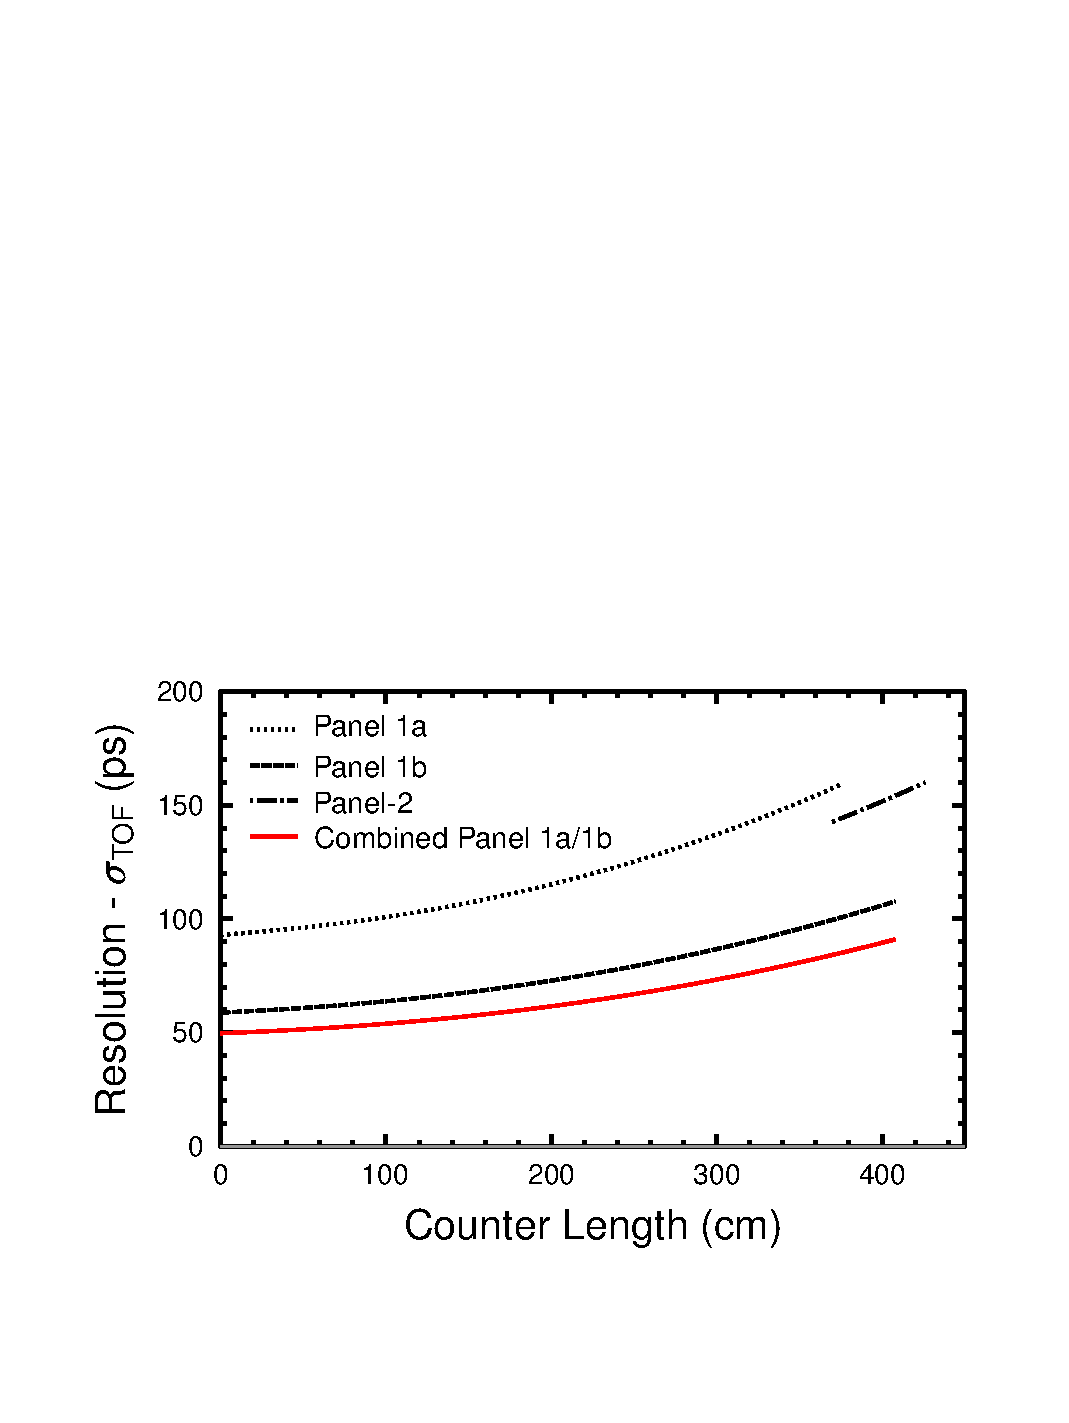
\includegraphics[width=1.0\textwidth,natwidth=610,natheight=642]{pics/resolution.pdf}}}
\end{picture} 
\caption{(Color Online) Parameterized expectation of the counter hit time resolution for the FTOF panel-1a
(dotted), panel-1b (dashed), and panel-2 (dot-dashed) counters as a function of length. The solid (red) line
indicates the final expected resolution in the forward direction by combining the hit time information from
the panel-1a and panel-1b counters. The horizontal line indicates the 80~ps average time resolution
specification for the FTOF system.}
\label{sigma_tof}
\end{figure}
%%%%%%%%%%%%%%%%%%%%%%%%%%%%%%%%%%%%%%%%%%%%%%%%%%%%%%%%%

\subsection{System Components}

\subsubsection{Scintillator Material}

To optimize the time resolution over the full volume of the FTOF counters, a scintillation material with a
fast time response and a long attenuation length are essential. For the panel-1a and panel-2 FTOF counters
that were refurbished from the older CLAS TOF system, Bicron BC-408 was selected. For the panel-1b
counters constructed for the new CLAS12 FTOF system, a different design approach was considered
that optimized the overall system timing resolution. For counters less than 2~m in length, the overall
performance is improved by the use of a faster scintillator with small decay times $\tau_{decay}$, whereas
for the longer counters, material with longer attenuation lengths is the better choice. The final decision
for the panel-1b counters was to use BC-404 for counters 1 $\to$ 31 (lengths from 17.3~cm to 209.4~cm)
and to use BC-408 for counters 32 $\to$ 62 (lengths from 215.8~cm to 407.9~cm). Table~\ref{scint-specs}
lists the properties of the FTOF scintillation materials.

%%%%%%%%%%%%%%%%%%%%%%%%%%%%%%%%%%%%%%%%%%%%%%%%%%%%%%%%%
\begin{table}[htbp]
\begin{center}
\begin{tabular}{c|c|c} \hline
Property                                    & BC-404     & BC-408  \\ \hline    
Light Output, \% Anthracene  & 68             &  64    \\ \hline
Rise Time (ns)                           & 0.7             & 0.9    \\ \hline
Decay Time (ns)                         & 1.8             & 2.1     \\ \hline
Pulse Width, FWHM (ns)         & 2.2              & 2.5    \\ \hline
Wavelength of maximum emission (nm) & 408    & 425 \\ \hline
Light attenuation length (cm)   & 140             & 210   \\ \hline
Bulk attenuation length (cm)     & 160             & 380  \\ \hline
Polymer base                             & \multicolumn{2}{c}{Polyvinyltoluene} \\ \hline
Refractive index                       & \multicolumn{2}{c}{1.58}                    \\ \hline 
Density (g/cm$^3$)                  & \multicolumn{2}{c}{1.023}                    \\ \hline 
\end{tabular}
\end{center}
\caption{The properties of the plastic scintillator material BC-404 and BC-408 employed for the counters
of the FTOF system~\cite{scint-mat-ref}.}
\label{scint-specs}
\end{table}
%%%%%%%%%%%%%%%%%%%%%%%%%%%%%%%%%%%%%%%%%%%%%%%%%%%%%%%%%

The bulk attenuation length of the scintillator material is stated by its manufacturer to be 160~cm for
BC-404 and 380~cm for BC-408. However, the practical attenuation length of the actual prepared bars
is smaller than this bulk value as the real path length of photons from the charged particle intersection
point to the ends of the bar is increased due to the finite geometry of the bar. For optimal response, this
practical attenuation length should be longer than the bar to ensure sufficient photon statistics.
Measurements of the practical attenuation length of the FTOF counters are given in Section~\ref{sec:attlen}.

\subsubsection{Photomultiplier Tubes and Voltage Dividers}

The panel-1a counters are read out at either end through 2-in diameter Thorn EMI 9954A PMTs (later
manufactured by ElectronTubes)~\cite{et-ref}. The PMTs were coupled to the scintillation bars using
12-cm-long Acrylic light guides that matched the 15~cm x 5~cm scintillator on one end and the 2~in
diameter PMT on the other end.  For the panel-2 counters Philips XP4312B/D1 3-in diameter PMTs (later
manufactured by Photonis~\cite{photonis}) are employed. The PMTs were coupled to the scintillators through
Acrylic light guides that matched the 22~cm x 5~cm scintillator on one end and to the 3~in diameter PMT
on the other end. Both the 9954A and XP4312B/D1 PMTs have 12 linear-focused dynode stages. For both
the panel-1a and panel-2 counters the PMTs are glued on the light guides using BC-600 optical glue. See
Ref.~\cite{tof-nim} for full details on the PMT selection criteria and the light guide designs. The
performance specifications for these PMTs are listed in Table~\ref{pmt-specs}.

The voltage dividers employed for the panel-1a and panel-2 readout were custom units built specifically for
the CLAS TOF project~\cite{tof-nim}. The dividers use high voltage field-effect transistors to fix the PMT
gain by stabilizing the voltage and to protect the PMT against high light levels by shutting down the circuit in
case of over-current. The grid voltage for both types of dividers followed the manufacturer's specifications.

The photomultipliers employed for the panel-1b counters are Hamamatsu R9779 2-in diameter PMTs integrated
with a voltage divider to form the R9779-20MOD assembly. These PMTs include 8 linear-focused dynode stages.
This high timing resolution PMT was selected due to its particularly compact overall length of $\sim$115~mm.
The length restriction was necessary to fit within the defined shadow region of the torus cryostats at the location
of the PMTs (see Section~\ref{ftof-geometry} for details). These PMTs are coupled directly to the ends of the
scintillation bars using BC-600 optical glue. The performance specifications for these PMTs are listed in
Table~\ref{pmt-specs}.

%%%%%%%%%%%%%%%%%%%%%%%%%%%%%%%%%%%%%%%%%%%%%%%%%%%%%%%%%
\begin{table}[htbp]
\begin{center}
\begin{tabular}{c|c|c|c} \hline
                                                           & 9954A                    & R9779                     & XP4312B/D1 \\ \hline
Property                                            & Panel-1a                   & Panel-1b                  & Panel-2 \\ \hline
Diameter                                           & 2~in                         & 2~in                        & 3~in \\ \hline
Photocathode area                            & 16.6~cm$^2$           & 16.6~cm$^2$        & 36.3~cm$^2$ \\ \hline
Dynode stages                                  & 12                            & 8                              & 12 \\ \hline
Spectral response                            & 290 $\to$ 680~nm & 300 $\to$ 650~nm & 290 $\to$ 650~nm \\ \hline
Max. wavelength emission               & 400~nm & 420~nm & 420~nm \\ \hline
Gain                                                    & 1.8$\times$10$^7$ & 5.0$\times$10$^5$ & 3$\times$10$^7$ \\ \hline
Quantum eff. @ $\lambda_{max}$   & 28\% & 28\% & 28\% \\ \hline
Max. anode current rating               & 100~$\mu$A & 100~$\mu$A & 100~$\mu$A \\ \hline
Anode dark current                         & 2~nA & 15~nA & 10~nA \\ \hline
Anode pulse rise time                      & 2~ns & 1.8 ns & 2.1 ns \\ \hline
Electron transit time                        & 41 ns & 20 ns & 31 ns \\ \hline
Transition time spread                     & 0.4~ns & 0.25 ns & 0.4 ns \\ \hline
\end{tabular}
\end{center}
\caption{The properties of the PMTs used for the readout of the FTOF panel-1a, panel-1b, and panel-2
counters. All of these PMTs have a borosilicate glass window and employ green-sensitive bialkali photocathodes.}
\label{pmt-specs}
\end{table}
%%%%%%%%%%%%%%%%%%%%%%%%%%%%%%%%%%%%%%%%%%%%%%%%%%%%%%%%%

\subsubsection{PMT Magnetic Shielding}

The FTOF PMTs are located roughly 600~cm to 700~cm from the target in a local magnetic field from
the torus computed to be less than 30~G when the torus is operated at full field. The magnetic shields
for the PMTs are included to reduce both the axial and transverse components of the field along the
full accelerating structure of the PMT to a level less than 0.2~G. For the panel-1a and panel-2 counters, the
PMT magnetic shields consist of a 0.020-in thick $\mu$-metal cylinder, with the shield extending 2-in
beyond the front face of the PMT.  For the panel-1b counters, the magnetic shields are composed of 2~mm
thick $\mu$-metal that extends 2-in beyond the front face of the PMT. The shield has a rectangular
box design that fits over the edge of the scintillation bar. The face of the shield opposite the PMT side
has a small penetration to allow the signal and HV cables and connectors to pass through. Further details
on the FTOF magnetic shielding and the field tests that were conducted are included in Ref.~\cite{ftof-shields}.

\subsubsection{Counter Assembly and Support}

Each scintillation counter is individually wrapped first with a reflective layer and then an opaque outer layer.
For panel-1a and panel-2 the scintillation counter wrapping materials include:

\begin{itemize}
\item 1 layer of 0.0094~in (0.02388~cm) thick black Kapton,
\item 2 layers of 0.001~in (0.00254~cm) thick aluminum foil,
\end{itemize}

\noindent
For panel-1b, the scintillation counter wrapping materials include:

\begin{itemize}
\item 3 layers of 0.0015~in (0.00381~cm) thick Tedlar,
\item 1 layer of 0.0003~in (0.00076~cm) thick aluminized Polyester film,
\end{itemize}

After wrapping, each of the FTOF scintillation counters was attached to a support structure that consists of
a composite sandwich structure of stainless steel skins on structural foam that is attached to the detector
frame only at the two ends. The composite structure, which mounts on the scintillator side facing away from
the target, provides uniform material thickness to the scattered particles.  The support was undersized so the
counters could be placed as close together as allowed by the wrapping material. 

Each panel-1a counter was mounted on 1-in-thick supports to minimize the thickness of the package from the
standpoint of Coulomb multiple scattering and energy loss considerations.  The maximum deflection for the
installed scintillators is 4.4~mm, as estimated from deflection tests and the compound angle of each detector,
which relieves the overall support requirements. The space for the panel-2 counters allowed for 3-in-thick
sandwich supports, which were mechanically much stiffer and resulted in no appreciable deflection. Again, each
panel-2 counter was mounted to its own support structure. For the panel-1b counters, the backing structures
were 2-in thick and designed to support two panel-1b counters. The maximum deflection for the installed
scintillators is less than 5~mm, which occurs at the middle of the longest counters.

The support structures onto which the scintillator counters were attached were bolted to box-beam support
frames (steel for panel-1a and panel-2, aluminum for panel-1b) that resided in the torus shadow regions. The
support frames were triangular in shape for panel-1a and panel-1b, and formed a rhombus shape for panel-2.
The panel-1a frames were bolted directly to the upstream faces of the electromagnetic calorimeters in each
sector of the Forward Carriage. The panel-1b frames were bolted directly to the panel-1a frames. The panel-2
frames were attach to the steel super-structure of the Forward Carriage.

\subsection{Electronics}
\label{sec-elec}

The outputs from the FTOF PMTs include both an anode and a dynode signal. The anode signals are
sent first to a discriminator and then to a TDC. The dynode signals are sent to a flash ADC. A block
diagram of the electronics layout for each FTOF counter is shown in Fig.~\ref{elec-block}.

For the FTOF PMTs the anode signal is roughly three times larger in amplitude than the dynode signal. For
the panel-1a and panel-2 PMTs, the dynode signals are bipolar with a negative polarity primary pulse with a
long tail that overshoots the baseline. This tail is not included in the determination of the pulse charge. For
the panel-1b PMTs, the anode signal has negative polarity and the dynode signal has positive polarity. To
ensure compatibility with the negative polarity input requirements of the FADC, the dynode signal is
inverted before the readout electronics using an inline Philips 460 IT inverting transformer.

The output from the panel-1b FADCs is also used as part of the CLAS12 level-1 trigger. Signals in
panel-1b above the FADC threshold are geometrically matched to cluster hits in the electromagnetic
calorimeter and to found tracks in the drift chambers to select charged hadrons. Signals from the FTOF
system are also used to provide an effective charged particle veto for the detection of neutrals in the
electromagnetic calorimeters. While high resolution timing measurements are the primary role of the
FTOF system for charged particle identification in the forward direction of CLAS12, the pulse height
information from the FADCs is also employed for energy loss measurements to provide an independent
means for identification of slow particles. In addition, pulse fitting techniques are employed using the
FADC pulse shape to determine the hit time of the track that can be matched to the TDC time to better
ensure matching of the ADC and TDC information in the high rate operating environment of CLAS12 (see
Section~\ref{cluster}.)

%%%%%%%%%%%%%%%%%%%%%%%%%%%%%%%%%%%%%%%%%%%%%%%%%%%%%%%%%
\begin{figure}[htbp]
\vspace{5.5cm}
\begin{picture}(50,50) 
\put(35,-30)
{\hbox{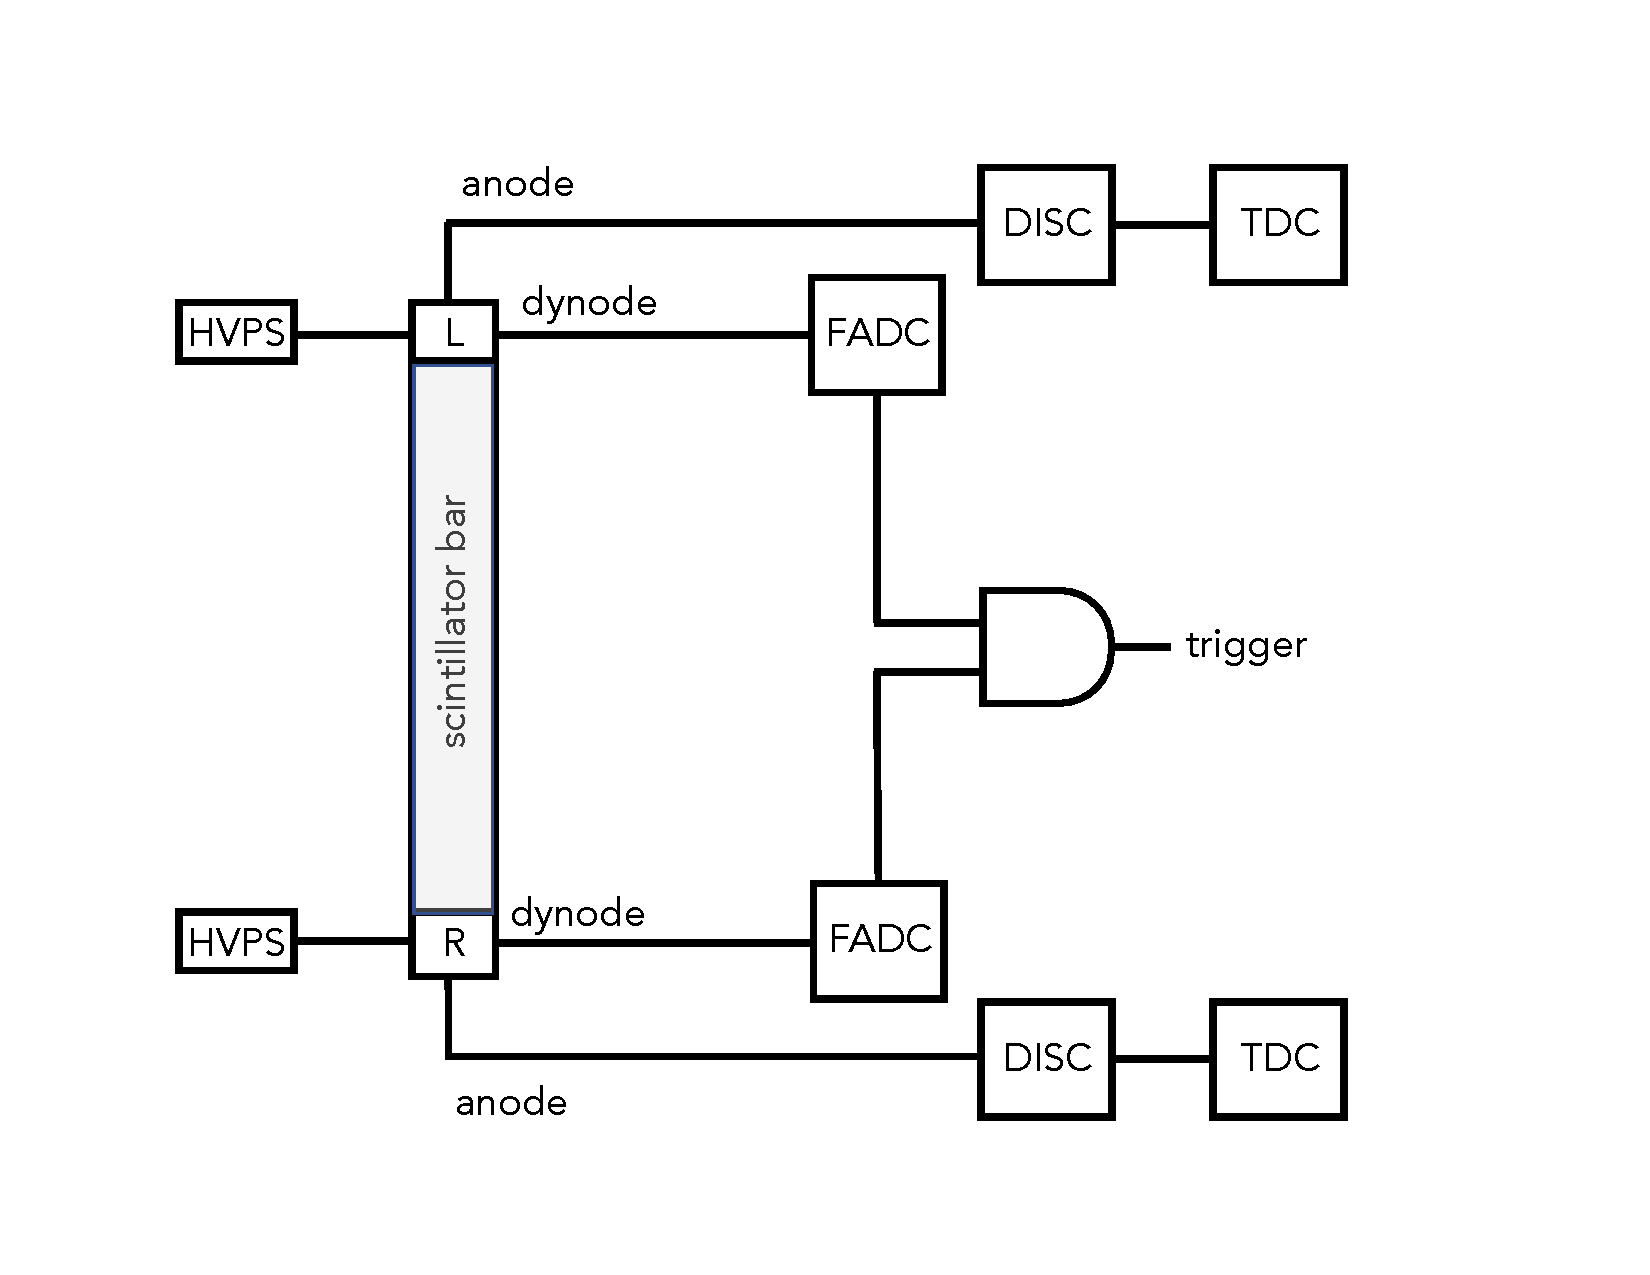
\includegraphics[width=0.65\textwidth,natwidth=610,natheight=642]{pics/ftof-electronics-block.pdf}}}
\end{picture} 
\caption{Schematic of the electronics for each counter in the CLAS12 FTOF system.}
\label{elec-block}
\end{figure}
%%%%%%%%%%%%%%%%%%%%%%%%%%%%%%%%%%%%%%%%%%%%%%%%%%%%%%%%%

The intrinsic resolution of the electronics system ($\sigma_0$) must be reduced in order that it not
provide a limitation to the effective counter timing resolution. There are several contributions to this
term and each electronic component was studied to understand its effect.  From our bench measurements
and measurements from CLAS12, a reasonable approximation for the floor term in the counter hit time
resolution is $\sigma_0=40$~ps (see Section~\ref{res-sec}). The PMT anode outputs are connected to
JLab-designed VME leading-edge discriminators. A leading-edge, rather than a constant-fraction,
discriminator was chosen for the FTOF system. Although a constant-fraction discriminator delivers better
timing initially, off-line time-walk corrections to leading-edge time give comparable results at a significantly
lower cost since the off-line analysis can use the measured charge. Time walk is an instrumental shift in the
measured hit time that arises due to the finite rise time of the analog pulse. For a given event time, pulses
of different amplitude cross the leading edge discriminator at slightly different time. The time-walk
correction algorithm is described in Section~\ref{sec-tw}. The discriminator threshold was set at -25~mV,
significantly above the 1-2~mV noise level. This threshold corresponds to $\sim$1~MeV of deposited
energy. The discriminator width was set to 35~ns in order to prevent multiple outputs from the same input
pulse.

The output of the discriminator goes to a CAEN VME TDC. Both high resolution TDCs (25~ps LSB CAEN
VX1290A) and lower resolution TDCs (100~ps LSB CAEN V1190A) are employed~\cite{tdc-manual}, where
the lower resolution TDCs are associated with the longer counters at large polar angles for panel-1a
($N_{counter}=17 \to 23$), panel-1b ($N_{counter}=49 \to 62$), and panel-2 ($N_{counter}=1 \to 5$). These
multi-hit pipeline TDCs were chosen in order to allow for readout capability in the operating luminosity of
$10^{35}$~cm$^{-2}$s$^{-1}$. The TDC readout window was set to 250~ns to ensure the full dynamic range
of the data was safely in time with the trigger. The key performance specifications of these units are given
in Table~\ref{tdcadc-specs}.

The integral non-linearity (INL) of the TDCs represents the accumulated error of the input-output
characteristic of the TDC with respect to the ideal response. This is defined by the function:

\begin{equation}
D(t) = \int \frac{t}{LSB},
\end{equation}

\noindent
where $D$ is the output data, $t$ is the input time, and $LSB$ is the bin size. The compensation tables
for the CAEN V1190A and VX1290A TDCs are stored as tables in the unit SRAM memory. Initial tables
are measured at the factory and come preloaded on the modules. These tables are reasonably accurate
when reading out the module using its internal 40~MHz/25~ns period clock. However, in CLAS12, the
modules are strobed with a clock of a slightly larger frequency of 41.67~MHz. This difference in the
frequency has a non-negligible affect the INL tables. For our purposes we use a high frequency pulser to
populate the full dynamic range of the TDC within the CLAS12 readout clock. The measured INL tables that
were derived from this calibration were written into the TDC memory to replace the factory-loaded values.
Details on the procedure and the residual non-linearity affects are given in Ref.~\cite{inl-tables}.

The PMT dynode outputs are connected to the FADCs for the pulse charge measurement. The readout
employs JLab-designed FADC250 16-channel VME 250~MHz flash ADCs are employed~\cite{fadc-manual}.
The JLab-250 FADC units can be operated in several readout modes. For standard data acquisition operation
the FTOF counters are readout in a mode where the pedestal is subtracted event-by-event.
Fig.~\ref{fadc-pulse} shows a raw ADC pulse from a representative FTOF PMT where the pedestal has not
been subtracted. Our procedure determines the pedestal over the first 15 channels. This average is
subtracted from our pulse signal region, which lies between channels 35 and 65. A pulse fitting algorithm
that fits the leading edge of the pulse down to the baseline is used to determine the hit time from the
FADC signal. The readout window for the FTOF FADCs is set to 192 samples (48~ns). The applied readout
threshold is set to $\sim$1~MeV to ensure that the hit cluster energy can be determined with a reasonable
accuracy. Details on the hit clusterization for FTOF are described in Section~\ref{cluster}. The key
performance specifications of these units are given in Table~\ref{tdcadc-specs}.

The signal cables used for the FTOF system to connect from the PMT anodes and dynodes to the Forward
Carriage patch panels were RG-58C/U fire-retardant coaxial cables. This type of cable is appropriate for
moderate length cable runs for fast signals with low signal distortion requirements. The cable runs vary
from 47~ft to 59~ft. The connections from the patch panels to the readout electronics were made with a
final 5~ft run of low loss RG-174 coaxial cable. The inline signal inverting transformers for the panel-1b
dynodes (see Section~\ref{sec-elec}) were attached directly to the Forward Carriage patch panels.

%%%%%%%%%%%%%%%%%%%%%%%%%%%%%%%%%%%%%%%%%%%%%%%%%%%%%%%%
\begin{table}[htbp]
\begin{center}
\begin{tabular}{c|c} \hline
TDC Specs (V1190A/VX1290A) & ADC Specs \\ \hline
No. Channels: 128/32             & 16               \\ \hline
RMS resolution 100~ps/25~ps          & Sampling 250 MHz \\ \hline 
Resolution: 19~bit/21~bit                  & Resolution: 12-bit \\ \hline
Inter-channel isolation $\le$ 3 LSB & Clock jitter 350~fs \\ \hline
Double-hit resolution 5~ns          & Data memory 8~$\mu$s \\ \hline    
Full-scale range 52~$\mu$s          & Trigger/Data latency 8~$\mu$s / 32~ns \\ \hline  
\multicolumn{2}{c}{Integral/Differential non-linearity} \\
$<$ 2.5 LSB / $<$ 3 LSB             & $\pm$0.5 LSB / $\pm$0.8 LSB \\ \hline
Inter-channel isolation $<$ 3 LSB   & SNR 56.8~dB @ 100~MHz input \\ \hline
\end{tabular}
\end{center}
\caption{The key performance specifications of the FTOF CAEN V1190A and VX1290A pipeline
TDCs and JLab FADC250 flash ADCs.}
\label{tdcadc-specs}
\end{table}
%%%%%%%%%%%%%%%%%%%%%%%%%%%%%%%%%%%%%%%%%%%%%%%%%%%%%%%%%

%%%%%%%%%%%%%%%%%%%%%%%%%%%%%%%%%%%%%%%%%%%%%%%%%%%%%%%%%
\begin{figure}[htbp]
\vspace{5.0cm}
\begin{picture}(50,50) 
\put(5,-45)
{\hbox{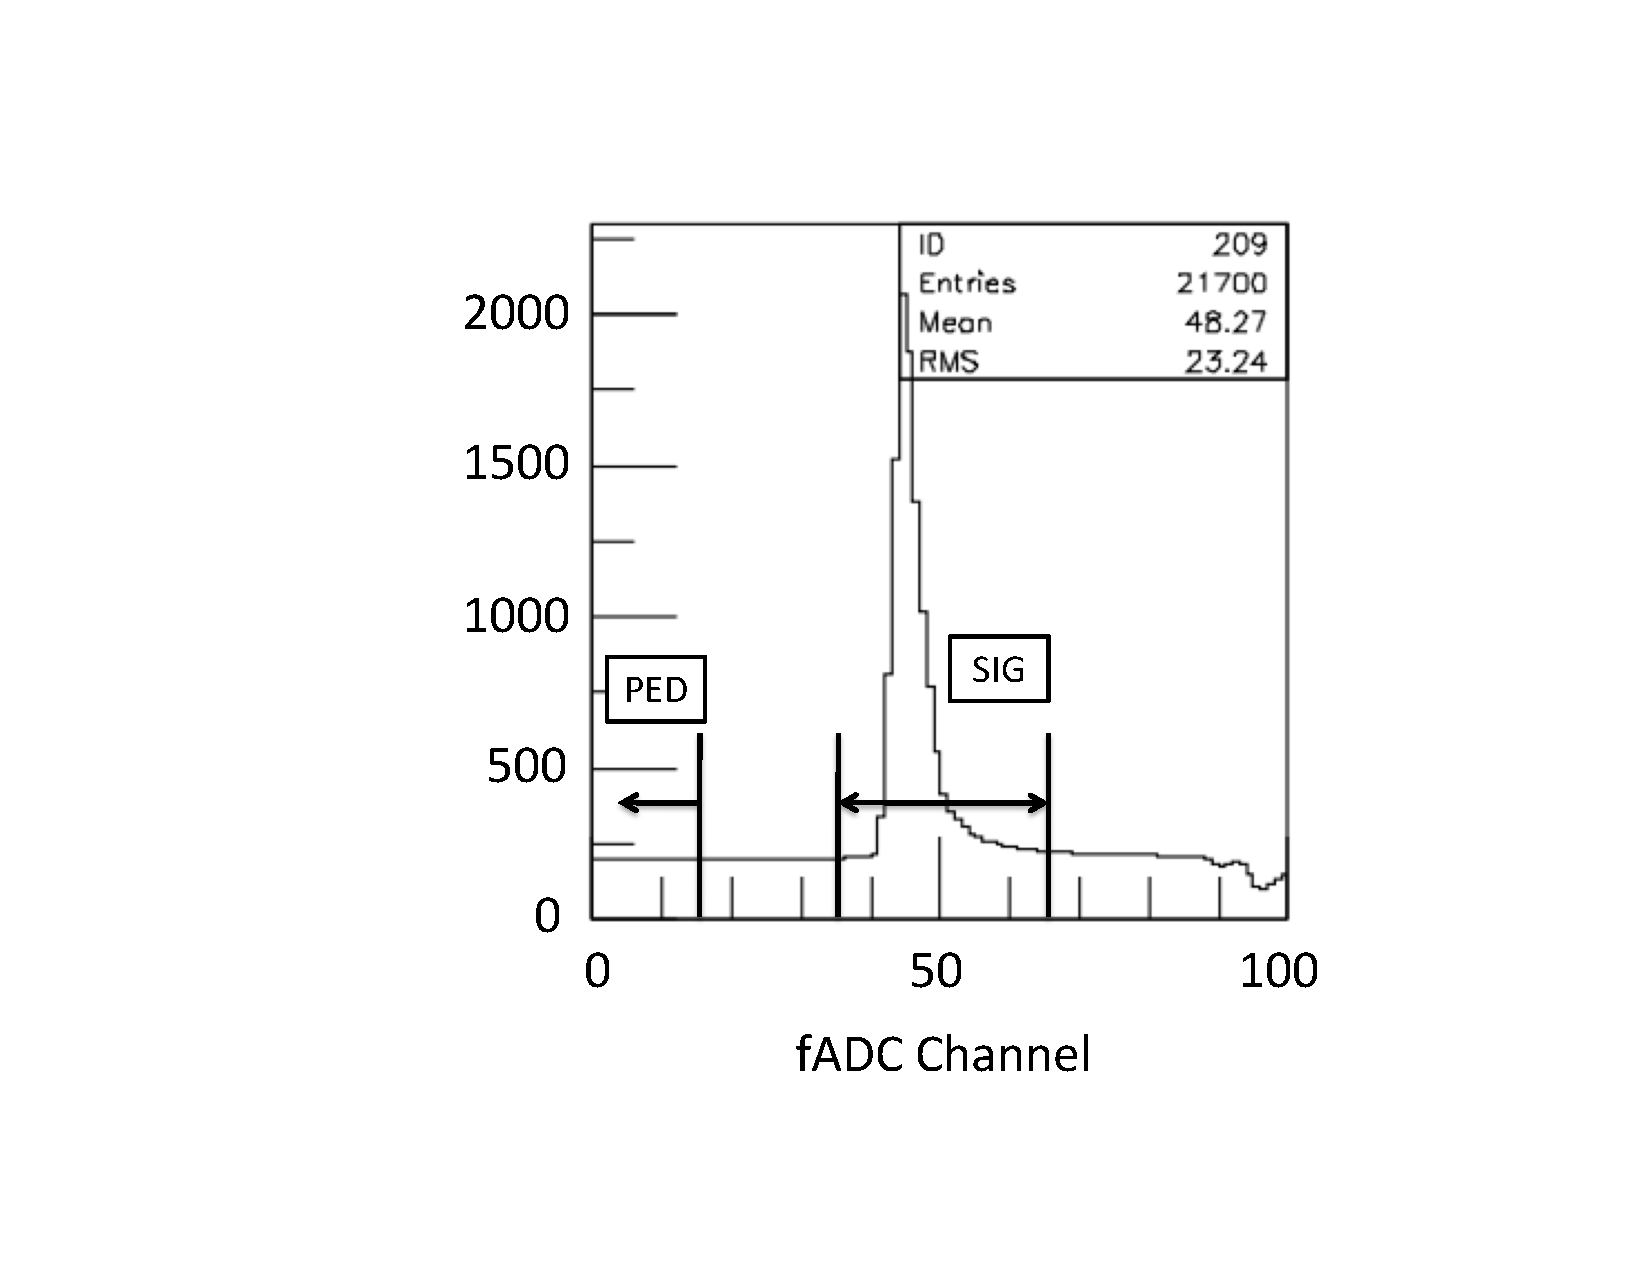
\includegraphics[width=0.65\textwidth,natwidth=610,natheight=642]{pics/fadc-pulse.pdf}}}
\end{picture} 
\caption{Typical FADC pulse from a representative FTOF counter with the JLab FADC250. The ``PED''
region is used to determine the average pedestal in the ``SIG'' region shown about the PMT pulse.}
\label{fadc-pulse}
\end{figure}
%%%%%%%%%%%%%%%%%%%%%%%%%%%%%%%%%%%%%%%%%%%%%%%%%%%%%%%%%

\subsubsection{High-Voltage Supplies}

The PMTs for the FTOF counters typically operate at about 2000~V with negative polarity. The typical
dark current drawn by the PMTs on the assembled counters was $<20$~nA. The system is powered by a
single high voltage mainframe for each sector. These mainframes are either CAEN 1527LC or CAEN 4527
units outfitted with negative polarity 24-channel A1535N modules that can supply up to 3.5~kV per channel
with a maximum current of 3~mA. The power supply has a voltage ripple specification of $<$20~mV
peak-to-peak (typical). Each channel consumes less than 1~W during counter operation. The typical supply
currents per channel are 300~$\mu$A to 500~$\mu$A.

The mainframe is controlled remotely through the Hall~B Slow Controls system. A graphical user interface
using EPICS~\cite{epics} running on a UNIX system communicates with the mainframe via Ethernet. The
mainframe settings enable basic protection of the PMTs in terms of maximum voltage and current settings,
and channel ramp rates.

The high voltage cables for each PMT are fire-retardant RG-59 coaxial cables that run from the voltage
divider to a local disconnect HV distribution box located behind the panel-2 arrays in each sector. There
are four HV distribution boxes for each sector, two for the left PMTs and two for the right PMTs of
each sector. The output of each HV distribution box is a pair of 35-ft-long multi-conductor cables, each
containing 24-channels, with a Radiall connector to mate with the HV A1535N board input connector. The
multi-conductor high voltage cables employed each contain 30 conductors wrapped in Tefzel insulation, and
outer wire shield and PVC insulation wrap. Each conductor is 5-kV rated.

\section{FTOF Performance}
\label{sec:performance}

This section highlights the performance of the FTOF system both on the test bench and in Hall~B
during the first beam runs for CLAS12. The bench test timing performance is important to
understand to ensure that both the refurbished counters that make up the panel-1a and panel-2
array from the CLAS TOF system still meet their original performance specifications as detailed
in Table~\ref{spec-table} and Ref.~\cite{tof-nim}. These bench performance studies are even more
important for the newly constructed panel-1b FTOF arrays for CLAS12 as they are primarily
responsible for the limits of the particle identification separation for CLAS12 in the forward direction.
Full details on the bench test performance results for the panel-1a and panel-2 counters are provided
in Ref.~\cite{dsc-cn2013-001} and for the panel-1b counters are provided in Ref.~\cite{nim-p1b}.

In this section the essential performance results from the bench testing studies in terms of the counter
photoelectron statistics and benchmark timing calibrations are presented. Then the nominal algorithms
are presented to provide details on how the in-beam FTOF timing resolution performance was calibrated
and quantified. Finally, this section provides the current status of the particle identification capabilities
of the FTOF system in relation to the design specifications.

\subsection{Bench Measurements}

\subsubsection{Counter Photoelectron Statistics}
\label{sec:npe}

The primary approach to determine the number of photoelectrons at the photocathode of the PMTs
generated by minimum-ionizing particles in the scintillation bars~(see Ref.~\cite{Gi86} for further details)
employs the ratio of the integral of the pulse for a minimum-ionizing particle to the integral of the pulse for a
single photoelectron. For these measurements we used the pulse integration feature of an Agilent
Technologies MSO-X 3034A 350~MHz (4 GSa/s) oscilloscope and averaged 1000 pulses. The
minimum-ionizing particle signals were analyzed connecting the scope to the PMT when mounted in position
on the shortest FTOF panel-1a counter. For the single photoelectron signal, we took data using just a bare PMT
on the bench using the same gain setting. For both measurements the oscilloscope threshold was adjusted
appropriately. For the minimum-ionizing peak analysis the threshold had to be set high enough ($>$200~mV)
to eliminate tracks that did not pass normally through the bar. For the single photoelectron peak the 
threshold had to be set low enough (1~mV) to pick out the noise pulses that were the source of the PMT
intrinsic dark current. This measurement scheme yielded $N_{pe}$=1000$\pm$100. This value is consistent
with that found during the initial characterization of these counters for the CLAS TOF system nearly
25 years ago~\cite{tof-nim}. Based on the parameterization given in Eq.(\ref{nphe-eq}), Fig.~\ref{nphe-plot}
shows the number of photoelectrons at the PMT photocathodes for the different FTOF counters.

%%%%%%%%%%%%%%%%%%%%%%%%%%%%%%%%%%%%%%%%%%%%%%%%%%%%%%%%%
\begin{figure}[htbp]
\vspace{3.8cm}
\begin{picture}(50,50) 
\put(33,-60)
{\hbox{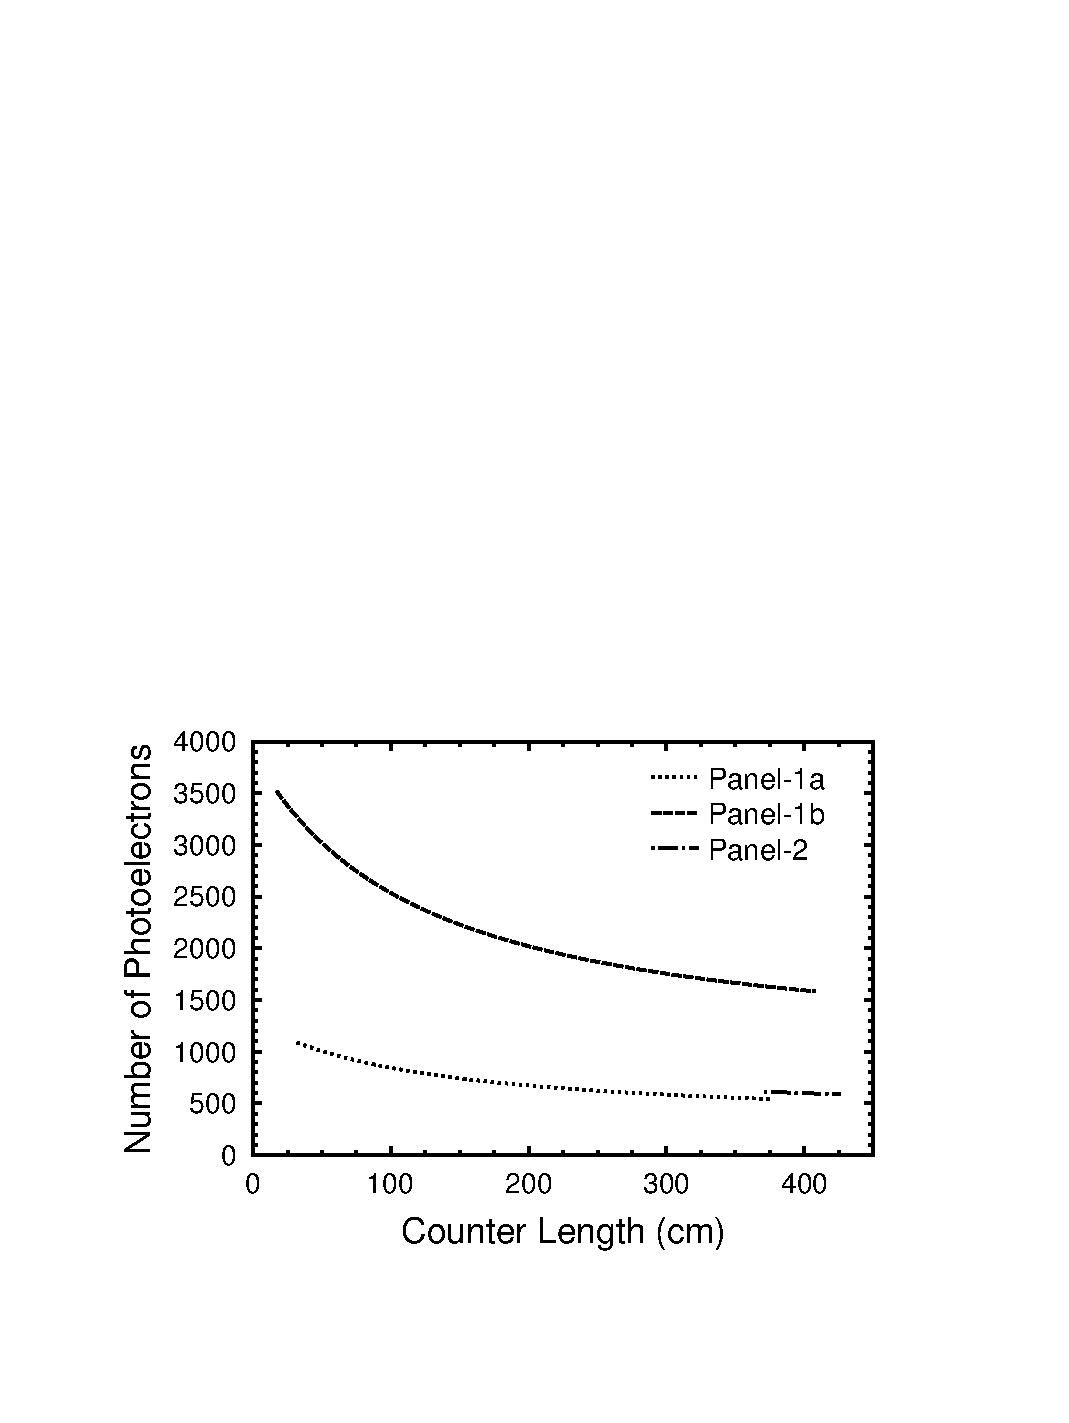
\includegraphics[width=1.0\textwidth,natwidth=610,natheight=642]{pics/nphe.pdf}}}
\end{picture} 
\caption{Parameterized distribution of the number of photoelectrons vs. counter length (cm) in the
different panel-1a (dotted), panel-1b (dashed), and panel-2 (dot-dashed) counters based on direct
measurements with the shortest panel-1a counter.}
\label{nphe-plot}
\end{figure}
%%%%%%%%%%%%%%%%%%%%%%%%%%%%%%%%%%%%%%%%%%%%%%%%%%%%%%%%%

A second method to determine the number of photoelectrons produced at the PMT photocathode,
which already accounts for the quantum efficiency at the photocathode, can be estimated from cosmic
ray data using the form~\cite{kajino}:

\begin{equation}
\label{nphe}
\langle N_{phe} \rangle = \left( \frac{M_{ADC}}{\sigma_{ADC}} \right)^2,
\end{equation}

\noindent
where $M_{ADC}$ is the ADC mean for the muon peak in the ADC spectrum and $\sigma_{ADC}$ is the width
of the ADC distribution. These quantities are most accurately determined from the system after the PMTs
are well gain matched. The form of Eq.(\ref{nphe}) assumes that a finite $\sigma_{ADC}$ arises solely due to
statistical variations in the number of photoelectrons created at the photocathode for an event sample with
a fixed energy loss per track, which we can assume to be a good approximation for normally incident
minimum-ionizing tracks. To determine the average number of photoelectrons based on Eq.(\ref{nphe}), it is
important that we minimize any attenuation length effects that lead to absorption of the scintillation light as
it propagates along the counter toward the PMTs. This can be done by restricting the coordinate along the
counter to within $\pm$5~cm about the center of the bar. From the measured data averaged across the
counters in panel-1a and panel-1b it was found that $N_{phe}^{1a} = 373 \pm 39$ and $N_{phe}^{1b} = 1158 \pm 77$
\cite{pmt-currents}. These results, while roughly a factor of two below the parameterized estimates also show
the same factor of three difference in the expected number of photoelectrons for panel-1b relative to panel-1a.
The estimates from the first approach are considered more reliable first because they are connected to a more
direct measurement of the number of photoelectrons, but also because this parameterization for $N_{phe}$
used in Eq.(\ref{timing-func}) agrees reasonably well with the measured counter resolutions shown in
Section~\ref{tres-beam}.

\subsubsection{Bench Time Resolution Performance}
\label{sec-bench}

The basic algorithm used on the test bench for the panel-1a and panel-2 counters to determine the time
resolution of a given reference counter is to use incident cosmic ray muon tracks to compare the measured
time for the reference counter to the time measured by two other identical counters in a triplet counter
configuration (see Fig.~\ref{triplet}). For a triplet measurement, where the track passes through all three
counters with double-sided readout, six times are measured ($t_1 \to t_6$). Each time measurement actually
represents the difference between the discriminated PMT signal (TDC start) and the trigger time (TDC stop
from the six PMT coincidence). These timing measurements are then translated into three counter hit times
$t_{t,m,b} = \frac{1}{2}(t_{1,3,5} + t_{2,4,6})$.

%%%%%%%%%%%%%%%%%%%%%%%%%%%%%%%%%%%%%%%%%%%%%%%%%%%%%%%%%
\begin{figure}[htbp]
\vspace{4.2cm}
\begin{picture}(50,50) 
\put(70,5)
{\hbox{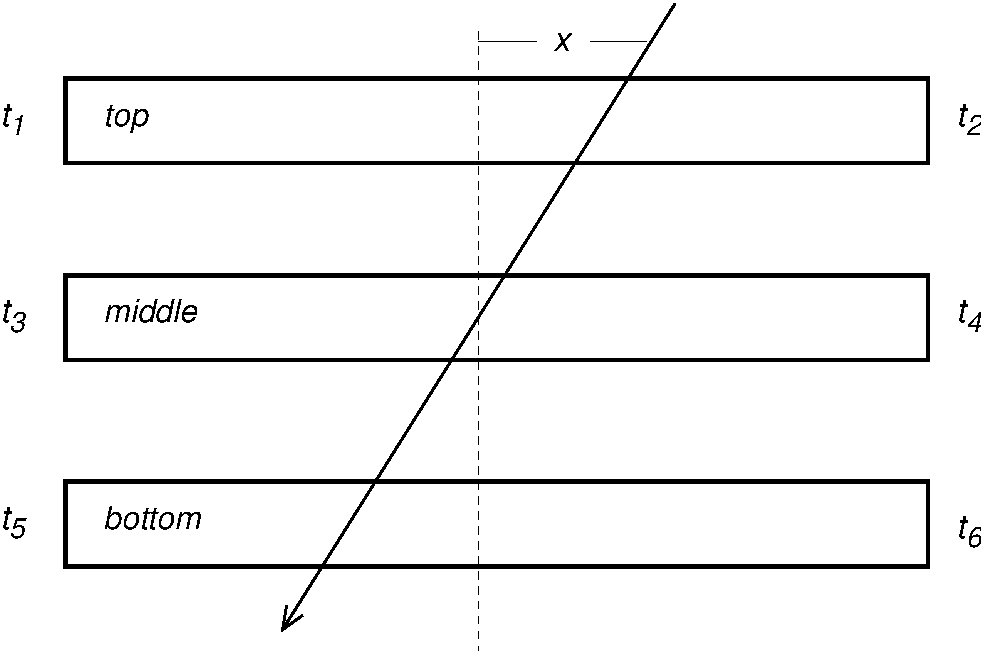
\includegraphics[width=0.80\textwidth,natwidth=610,natheight=642]{pics/triplet-alt.pdf}}}
\end{picture} 
\caption{Schematic representation of a triplet of counters (labeled top - t, middle - m, bottom - b) with a
muon track traversing the stack. The geometry of the triplet is configured such that the separation between
the top and middle counters matches that of the middle and bottom counters.}
\label{triplet}
\end{figure}
%%%%%%%%%%%%%%%%%%%%%%%%%%%%%%%%%%%%%%%%%%%%%%%%%%%%%%%%%

For incident tracks that pass fully through each counter of the triplet with measured times $t_t$, $t_m$,
and $t_b$, we can define a time residual $t_r = t_m - \frac{1}{2}(t_t + t_b)$, where we should expect that
the time $t_m$ of the middle scintillator hit should be the average of the measured times $t_t$ and $t_b$
for the top and bottom scintillator hits, respectively. Thus the measured residual $t_r$ should nominally be 0.
However, due to the smearing of the measured times $t_t$, $t_m$, and $t_b$ due to the finite time resolution
of the measurements, the residual time $t_r$ will also be smeared. While we still expect the mean of $t_r$ to
be zero, the width of the $t_r$ distribution can be used to determine the average time resolution of each
counter in the triplet. (For the outer counters in the triplet, the definition of the time residual must be slightly
modified to account for the small path length difference between the reference counter and the other two
counters.)

The average time resolution of each counter is computed from the variance $\delta t_r$ in the measured time
residual $t_r$. Assuming the average time resolution for each PMT in the triplet ($\Delta t_i$, $i = 1 \to 6$)
is identical and taking into account that each counter is readout using two PMTs, we can write the final expression
for the average counter timing resolution as:

\begin{equation}
\label{sig-counter}
\sigma_{counter} = \frac{2}{\sqrt{6}} \delta t_r.
\end{equation}

\noindent
Thus a measure of the width ($\sigma$) of the time residual distribution provides a measure of the average
resolution of each counter in the triplet. 

Fig.~\ref{final-resolution} shows the average timing resolution measured for the triplet configurations for the
panel-1a and panel-2 FTOF counters. For these measurements the fully assembled counter arrays were stacked
one above the other in the cosmic ray test stand. The triplets were formed from the counters for Sectors~1, 6,
and 5 and separately for the counters for Sectors~2, 4, and 3. This analysis included a minimum PMT ADC cut to
remove events that did not pass through the full thickness of the counter (``corner-clippers'') and also included a
coordinate cut of $\pm$10~cm about the center of the scintillation bar. Due to the use of leading edge
discriminators the measured PMT times were corrected with a time-walk function of the form:

\begin{equation}
\label{walk-function}
t_{walk}^{L,R} = \frac{A_0}{1 + A_1 \sqrt{(ADC - PED)_{L,R}}}.
\end{equation}

\noindent
Here, $ADC - PED$ is the pedestal-subtracted ADC value for each PMT. The time-walk functional in
these measurements best described the data using $A_0 = 50.0$ and $A_1 = 0.852$.

The average time resolutions for the counters in the panel-1a S1-S6-S5 and S2-S4-S3 triplets were
found to be slightly better ($\sim$15\%) than that achieved for the baseline measurements over
20~years ago. For panel-2, the average time resolution was found to be slightly worse ($\sim$15\%)
than these same baseline measurements.

%%%%%%%%%%%%%%%%%%%%%%%%%%%%%%%%%%%%%%%%%%%%%%%%%%%%%%%%%%%%%%
\begin{figure}[htbp]
\vspace{3.0cm}
\begin{picture}(50,50) 
\put(0,-60)
{\hbox{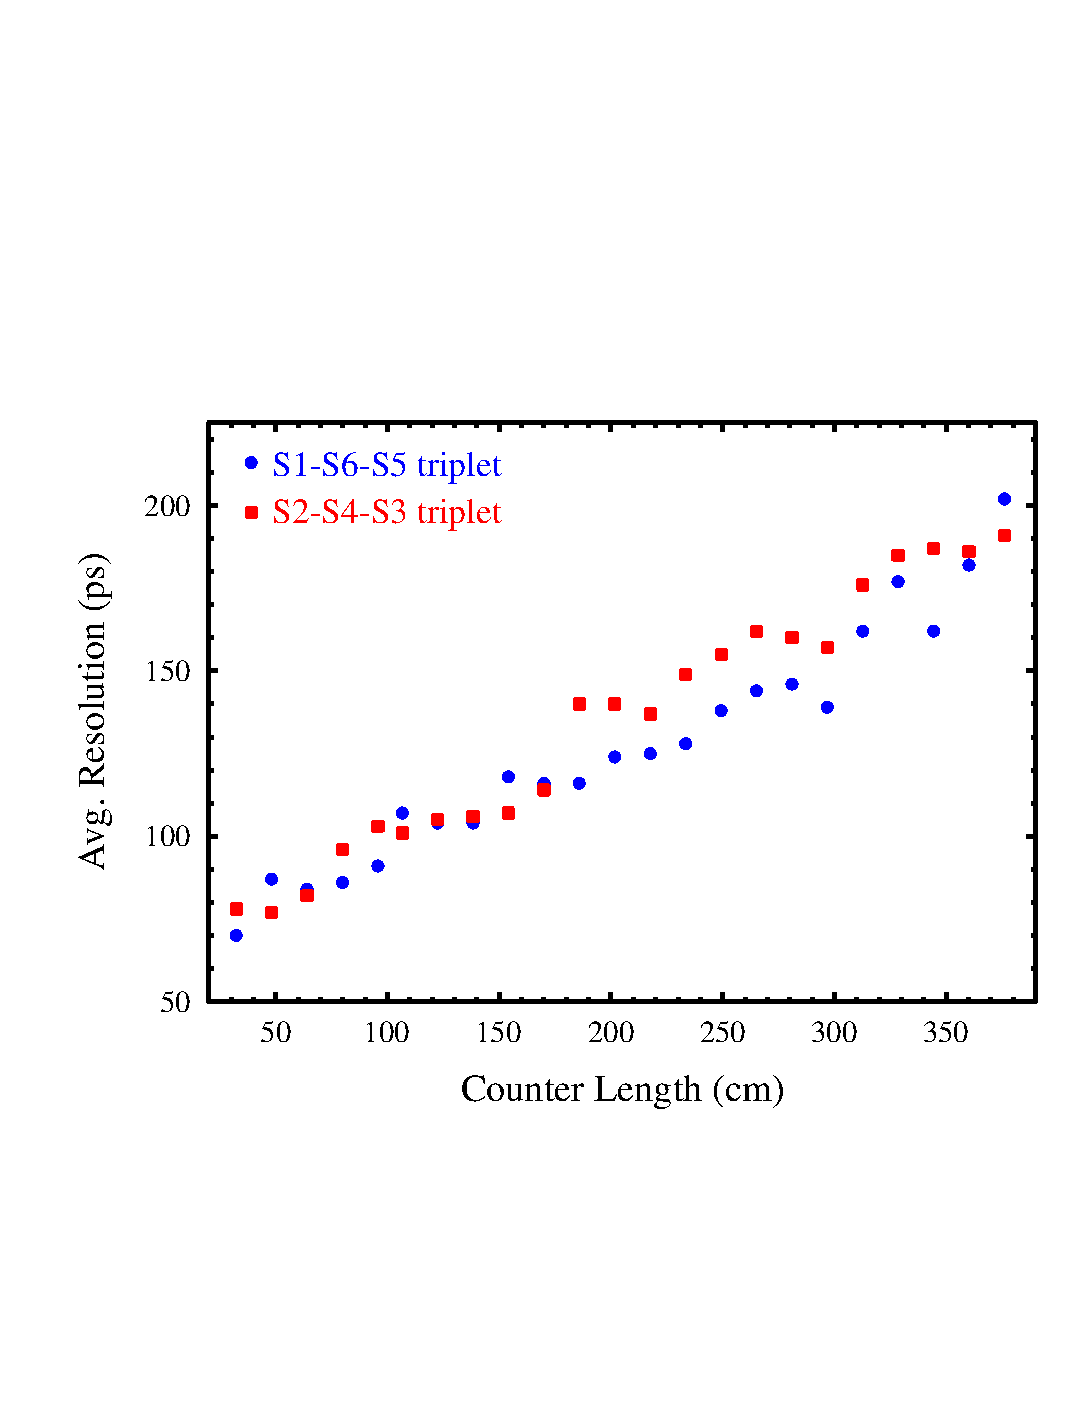
\includegraphics[width=0.60\textwidth,natwidth=610,natheight=642]{pics/p1a-tres.pdf}}}
\end{picture} 
\begin{picture}(50,50) 
\put(135,-60)
{\hbox{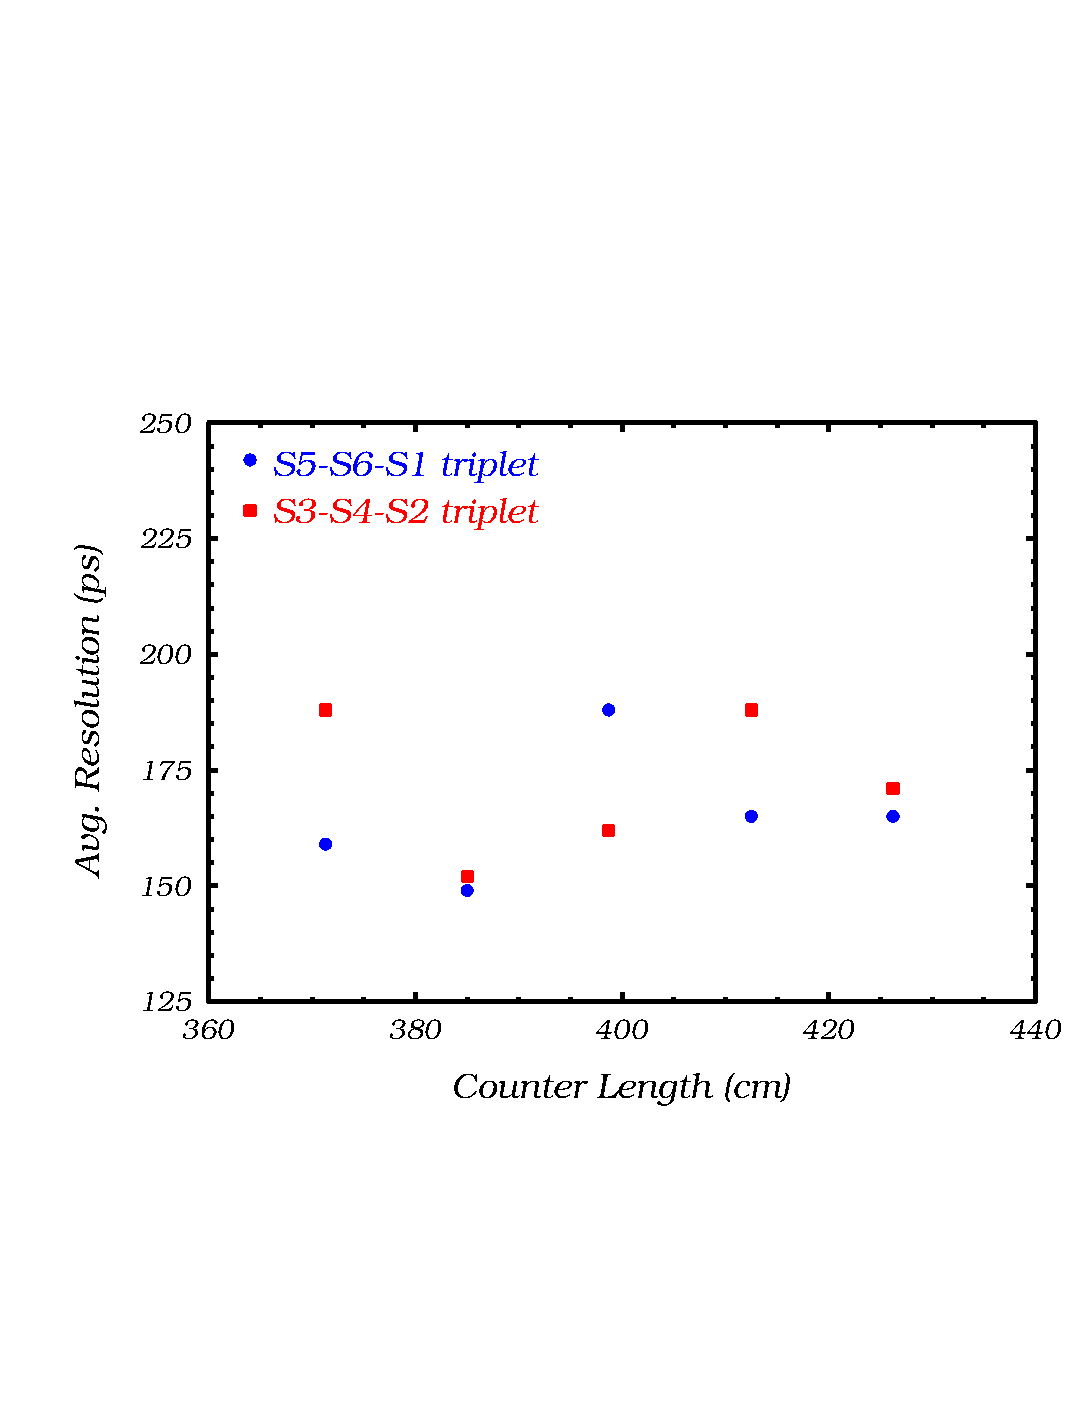
\includegraphics[width=0.60\textwidth,natwidth=610,natheight=642]{pics/p2-tres.pdf}}}
\end{picture} 
\caption{(Color Online) Average bench measurement resolutions (ps) vs. counter length (cm) using cosmic ray
muons for the refurbished FTOF panel-1a (left) and panel-2 (right) counters. The different sets of data points
correspond to the two different cosmic ray test stands used for calibration. The data points for the counters
in sectors 1, 5, and 6 were averaged together and the data points for the counters in sectors 2, 3, and 4 were
averaged together.}
\label{final-resolution}
\end{figure}
%%%%%%%%%%%%%%%%%%%%%%%%%%%%%%%%%%%%%%%%%%%%%%%%%%%%%%%%%%%%%%%%%

The bench measurements for the panel-1b FTOF counters were carried out using a stack of six identical
counters from $N_{counter} = 1 \to 62$. The approach to determine the average time resolution for a given
$N_{counter}$ was similar to that for the measurements of the panel-1a and panel-2 triplets. Again, the 
measured time for a given reference counter in the stack of six counters was compared to the average time
measured by the other five. Accounting for the necessary path length corrections to relate the reference
counter time to the five-counter average time, a time residual generalized from that in Eq.(\ref{timing-func})
was employed again assuming that the PMT time resolution was the same for all 12 gain-matched PMTs in the
sextet test stand configuration. Also in distinction to the simple time-walk correction employed for the panel-1a
and panel-2 measurements shown in Eq.(\ref{walk-function}), a more sophisticated position-dependent time-walk
correction was employed that generalized the simpler position-independent form. Precision measurements of the
time-walk amplitude ($A_0$ in Eq.(\ref{walk-function})) vs. the distance from the PMT showed a nearly linear
fall-off of the amplitude with increasing distance from the PMT. On average the time-walk amplitude is $\sim$30\%
larger at the PMT compared to the far end of the bar, although this near end to far end ratio of the amplitude
decreases linearly with the length of the bar. Our measurements showed this ratio varies between 20\% for the
shortest bars to 40\% for the longest bars. After accounting for this correction vs. hit position along the bar, a
final baseline for the average panel-1b time resolutions were extracted averaging over the six identical counters
from $N_{counter} = 1 \to 62$. The final bench measurement results are shown in Fig.~\ref{p1b-tres}. The timing
resolutions for the panel-1b counters shown in Fig.~\ref{p1b-tres} range from 30~ps for the shortest counters 
(17~cm long) to 80~ps for the longest counters (408~cm long). Full details describing these measurements are
provided in Ref.~\cite{nim-p1b}.

%%%%%%%%%%%%%%%%%%%%%%%%%%%%%%%%%%%%%%%%%%%%%%%%%%%%%%%%%%%%%%%%
\begin{figure}[htbp]
\vspace{4.2cm}
\begin{picture}(50,50) 
\put(50,-85)
{\hbox{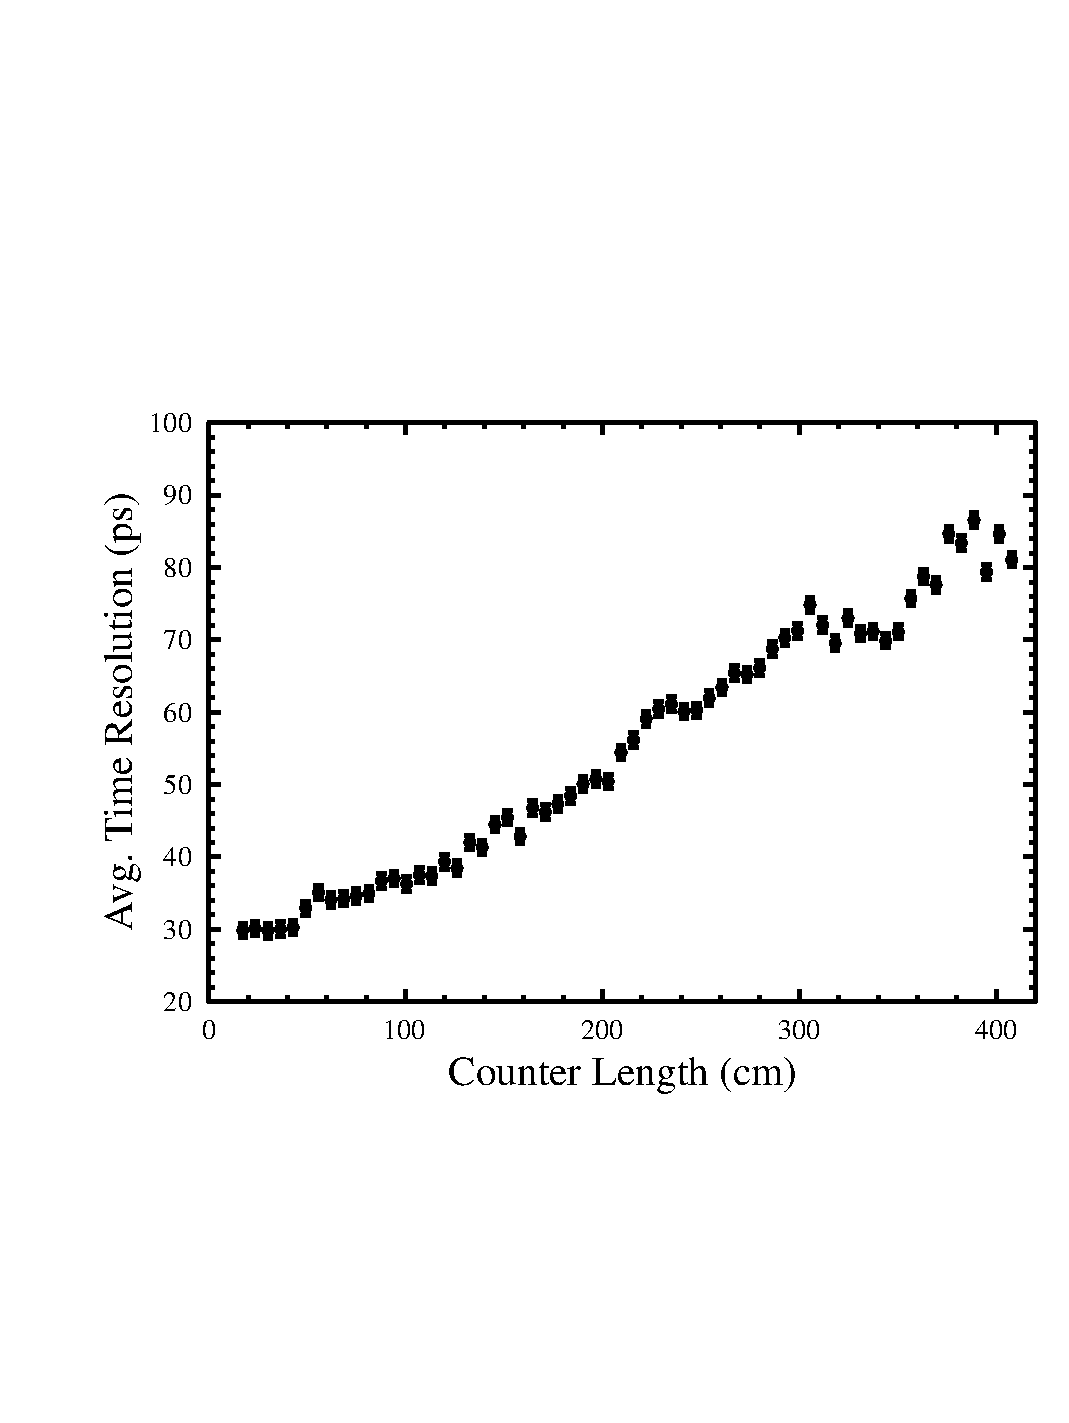
\includegraphics[width=0.8\textwidth,natwidth=610,natheight=642]{pics/p1b-tres.pdf}}}
\end{picture} 
\caption{Measurements of the time resolution (ps) vs. counter length (cm) achieved for the FTOF panel-1b
system averaged over the six identical counters belonging to each CLAS12 Forward Carriage sector. These
data were acquired on the bench using cosmic ray muons. Full details are included in Ref.~\cite{nim-p1b}.}
\label{p1b-tres}
\end{figure}
%%%%%%%%%%%%%%%%%%%%%%%%%%%%%%%%%%%%%%%%%%%%%%%%%%%%%%%%%%%%%%%%

For our purposes in quoting counter time resolution values, it is essential to distinguish between two different
quantities. the first is the {\em intrinsic} counter time resolution that reflects the resolution defined in
Eq.(\ref{timing-func}). This includes the resolution contributions mainly due to photon statistics at the PMT
photocathode due to the counter geometry, surface quality, scintillation material and bulk quality, wrapping
preparations, etc., the transit time spread of the PMT, and the readout electronics noise (the floor term of the
resolution). However, when calibrating the time resolution in situ in Hall B with beam interactions in the experimental
target, an {\em effective} time resolution is extracted that includes not only the intrinsic resolution contributions but
also contributions from the angle-dependent uncertainty in the path length determined by the CLAS12 forward tracking
system and the resolution spread in the accelerator RF signal that is used as a comparison reference time. The
results quoted in this section represent the intrinsic time resolutions of the counters. The effective in situ
time resolutions are discussed in detail and presented in Section~\ref{tres-beam}.

\subsection{FTOF Beam-Data Calibrations}

In the nominal data taking mode for CLAS12, whenever the FTOF is involved in an event that triggers the
spectrometer, the ADCs and TDCs for all PMTs with a signal above the discriminator threshold are recorded.
For the FADCs, the charge of the pulse is integrated over the extent of the pulse region and the pedestal is
subtracted event by event as discussed in Section~\ref{sec-elec}. For the TDCs the time recorded is relative
to the trigger. To determine the flight time of the charged track from the target to the FTOF, the TDC time
must be compared to the time of the accelerator radio frequency (RF) pulse relative to the trigger.  The RF
signal from the accelerator has a period an integer multiple of 2.004~ns. The RF bunch length itself corresponds
to a few picoseconds. Although the timing signals are very accurate (with a resolution of $<$20~ps), the
determination of which beam bunch produced a given interaction must be determined by the experiment.

The full calibration of the each of the FTOF counters involves a number of discrete steps that are carried out
separately for each of our data runs (where a run typically lasts for about two hours). The calibration constants
for each run are stored in the CLAS12 calibration database. The steps to the FTOF calibration are carried out
in a particular sequence~\cite{ftof-calib}.

\begin{enumerate}
\item Left/right PMT time offsets: This time offset accounts for the difference in the time recorded
between the left side and right side PMTs in a given counter due mainly to the different PMT transit times.
These time offsets are determined by determining the centroid of the difference between the left/right
TDC time difference and the left/right TDC time difference computed using the counter hit point from the
drift chamber system divided by the effective speed of light in the counter. These time shifts range between
$\pm$5~ns.

\item ADC Calibration: Determine the ADC channel to energy deposition calibration factor for each counter
using minimum-ionizing events. See Section~\ref{gain-matching}.

\item Attenuation Length Calibration: This property of the counter quantifies the light absorption length and
is determined by relating the measured ADC as a function of hit coordinate along the bar. See
Section~\ref{sec:attlen}.

\item Effective Velocity Calibration: Determine the effective speed of light propagation along the counter. See
Section~\ref{sec:veff}.

\item Time-Walk Amplitude Calibration: Compare the measured hit time with respect to the measured ADC to
determine the time-walk correction amplitudes. See Section~\ref{sec-tw}.
  
\item Counter-to-Counter Time Offset Calibration. In order to measure the absolute flight time of a charged
particle from the target to the FTOF counter and to be able to reconstruct exclusive events when hits are
associated with multiple FTOF counters, the relative time offsets of each counter relative to all of the other
counters in the system need to be determined. This is done in two steps for the FTOF calibration. The first
step is to align each track to the RF time, a step that amounts to a precision time alignment in bins of the TDC
LSB. The second step is a coarse alignment of each counter time in bins of the RF period $T_{RF}$. See
Section~\ref{sec-talign}. During this same step the effective counter timing resolutions are extracted. See
Section~\ref{tres-beam}.

\item TDC Calibration: After calibrating the integral non-linearities of each TDC channel in the system (see
Section~\ref{sec-elec}), the TDC channel to time calibration is completed using beam events. See
Section~\ref{sec-tdccal}.

\end{enumerate}

\subsubsection{Gain Matching}
\label{gain-matching}

One of the purposes of gain-matching the FTOF PMTs is to equalize the detector response to tracks that
cross the FTOF arrays such that two counters are involved. This is a necessary procedure because each
counter must contribute equally to the trigger for a common-threshold discriminator level. Gain matching
so that the minimum-ionizing particle response is such that the peak location appears in the same ADC
channel for all counters also allows for easier data monitoring during online and offline analysis.

The FTOF PMT high voltage settings were determined using calibration runs employing minimum-ionizing tracks.
These minimum-ionizing tracks deposit roughly 10~MeV (12~MeV) as they pass through the 5~cm (6~cm) thick
FTOF scintillation bars, as $dE/d\rho x = 2$~MeV/g/cm$^2$ for minimum-ionizing particles. Normally the high
voltage settings are based on runs using cosmic ray muons with the readout based on a calorimeter pixel trigger
that effectively selected tracks approximately normal to the face of the FTOF counters in panel-1a and panel-1b.
These calibrations can also be carried out using minimum-ionizing tracks from beam data coming from the target.
In this case the charge information is scaled by a path length correction given by $t/P$, where $t$ is the counter
thickness and $P$ is the path-length of the track in the counter as determined by extrapolation of the drift
chamber track to the location of the FTOF counter.

The energy deposited in the scintillation bars follows a Landau distribution for the minimum-ionizing
tracks. The energy deposited is recorded by the ADCs, which show a peak above pedestal for the tracks. Tracks
that do not pass through the full counter thickness and non-minimum-ionizing tracks give rise to a background
beneath the Landau peak.

For the HV calibrations, to avoid issues with the attenuation of light for tracks that pass near the ends of the
bars and to avoid issues with unbalanced light entering the left and right PMTs, we combine the information
from the left and right PMTs to produce an average ADC spectrum for the counter through the quantity known
as the ADC geometric mean given by:

\begin{equation}
\label{adc}
\overline{ADC} = \sqrt{ (ADC - PED)_L \cdot (ADC - PED)_R}.
\end{equation}

Given the finite dynamic range of the ADC, we have chosen to position the minimum-ionizing muon peak in a
particular ADC channel that is different for the panel-1a, panel-1b, and panel-2 counters. For all counters
this channel is selected so that it is safely above the pedestal, but leaves sufficient range for the more
highly ionizing charged tracks of our typical physics events. To minimize PMT aging effects that result in
loss of PMT gain with time due correlated with the total charge collected at the first dynode of the
accelerating structure, the PMT gains are set as low as possible.

The position of the muon peak in the ADC spectrum is set by the PMT HV values. For a given scintillation
bar, the typical average ADC spectrum appears as shown in Fig.~\ref{gmean}. Given that the same channel
is chosen to position the minimum-ionizing peak for all counters in a given panel-1a or panel-1b panel, this
implies that the PMT gain linearly increase in going from the short bars to the long bars to compensate for
the attenuation losses in the longer bars.

%%%%%%%%%%%%%%%%%%%%%%%%%%%%%%%%%%%%%%%%%%%%%%%%%%%%%%%%%
\begin{figure}[htbp]
\vspace{4.5cm}
\begin{picture}(30,50) 
\put(95,-50)
{\hbox{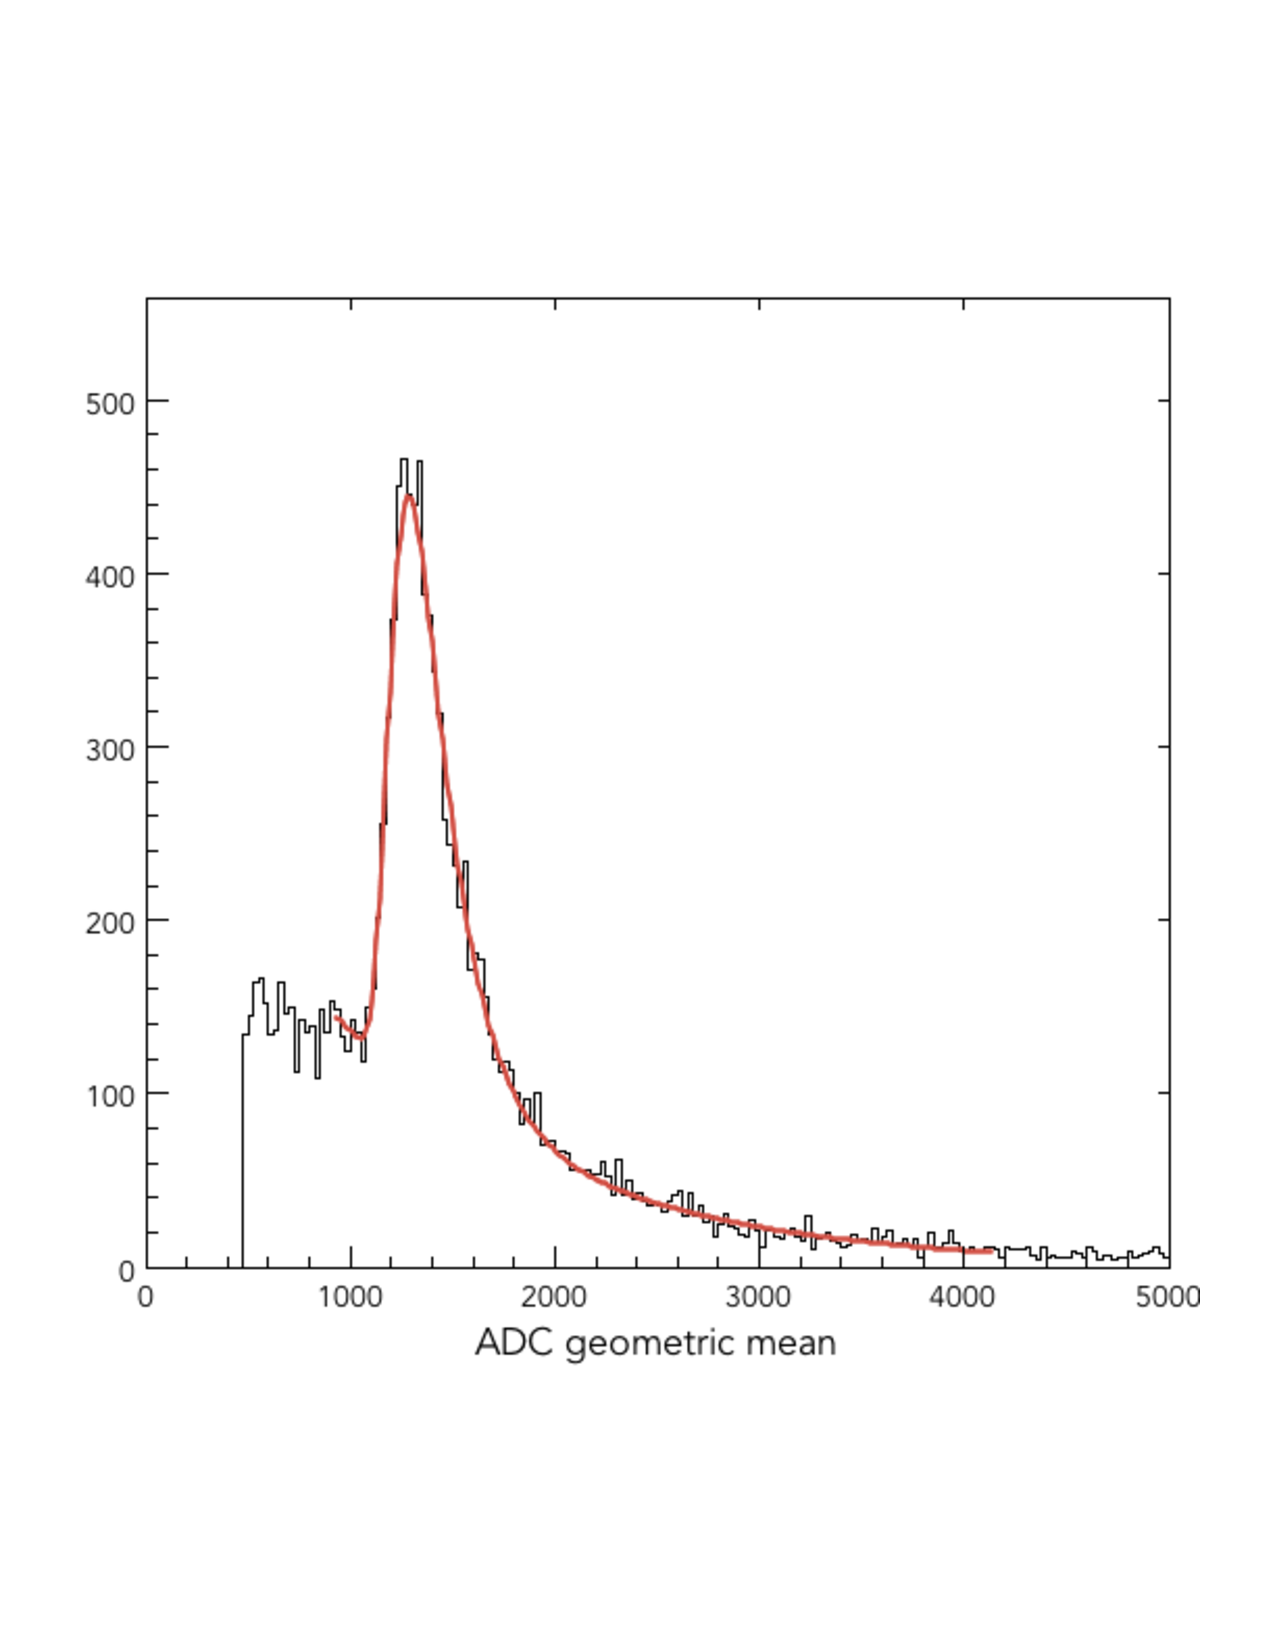
\includegraphics[width=0.53\textwidth,natwidth=610,natheight=642]{pics/gmean.pdf}}}
\end{picture} 
\caption{(Color Online) Geometric ADC mean for one representative FTOF counter from beam data
in CLAS12. The events recorded in the ADC spectrum have been pedestal subtracted. The red curve
is the fit function that includes a Landau shape for the peak and an exponential for the background.}
\label{gmean}
\end{figure}
%%%%%%%%%%%%%%%%%%%%%%%%%%%%%%%%%%%%%%%%%%%%%%%%%%%%%%%%%

The PMT gains depend exponentially on the applied voltage. Expressed in a slightly different way, we 
can relate the PMT gain $G_1$ at a given voltage $V_1$ to the gain $G_2$ at a different voltage $V_2$ 
via:

\begin{equation}
\label{power-law}
\frac{G_1}{G_2} = \left( \frac{V_1}{V_2} \right) ^\alpha.
\end{equation}

\noindent
This is a basic power law form with $\alpha$ representing the power law factor. Rewriting 
Eq.(\ref{power-law}) in a slightly different form, we have:

\begin{equation}
\label{delta}
\frac{\Delta G}{G} = \alpha \frac{\Delta V}{V}.
\end{equation}

It is this expression that is the basis for relating the position of the muon peak in the 
$\overline{ADC}$ spectrum (see Eq.(\ref{adc})) to the PMT HV setting. The gain-matching 
procedure then amounts to adjusting the HV settings of all PMTs to the values required to 
position the muon peak for each counter in the desired ADC location. At the same time the 
algorithm uses the individual left and right PMT ADC spectra for a given counter to 
ensure that these PMT gains are balanced.

The determination of the power law factor $\alpha$ in Eq.(\ref{power-law}) for each PMT
type can be determined looking at data with two different high voltage settings. In this manner
the average $\alpha$ factors for the FTOF PMTs were determined to be 13.4 for panel-1a,
4.7 for panel-1b, and 8.6 for panel-2. With these values the calibrations converge within just
a few iterations such that all of the minimum-ionizing particle peak locations are within
$\pm$25 ADC channels of their set targets.

The energy loss in a counter for a passing charged particle track is determined after the
minimum-ionizing peak centroids are aligned. The computed energy loss in each counter is
computed from each PMT as:

\begin{equation}
E_{L,R} = ADC_{L,R} \cdot \left [ \frac{\left( \frac{dE}{dx} \right)_{MIP} \cdot t}{ADC_{MIP}}\right ]
\exp\left(\frac{d_{L,R}}{\lambda}\right),
\end{equation}

\noindent
where $ADC_{MIP}$ is the centroid of the minimum-ionizing peak in the geometric mean distribution,
$\left( \frac{dE}{dx} \right)_{MIP}$ is the energy loss for minimum-ionizing particles in the scintillation
bars (1.956~MeV/cm), $t$ is the counter thickness ($t$=5~cm for panel-1a, panel-2, and $t$=6~cm for
panel-1b), $d$ is the distance along the bar from the track hit position to the PMT and $\lambda$ is the
counter attenuation length. The energy loss used in the event reconstruction is the geometric mean of the
separate measures $E_{L,R}$.

Fig.~\ref{ftof-dedx} shows the reconstructed energy loss normalized by the track path length through
the bar for the different counters from a data run with a 10.6~GeV electron incident upon a liquid-hydrogen
target. The data allow the separation of minimum-ionizing particles from more heavy ionizing particles.
The minimum-ionizing particles lose a constant energy as a function of path length. The heavy ionizing
particles have energy loss that increases linearly with distance at low momentum until they can pass
through the counter. At that point their energy loss follows the Bethe-Bloch formula.

%%%%%%%%%%%%%%%%%%%%%%%%%%%%%%%%%%%%%%%%%%%%%%%%%%%%%%%%%
\begin{figure}[htbp]
\vspace{5.0cm}
\begin{picture}(50,50) 
\put(-2,270)
{\hbox{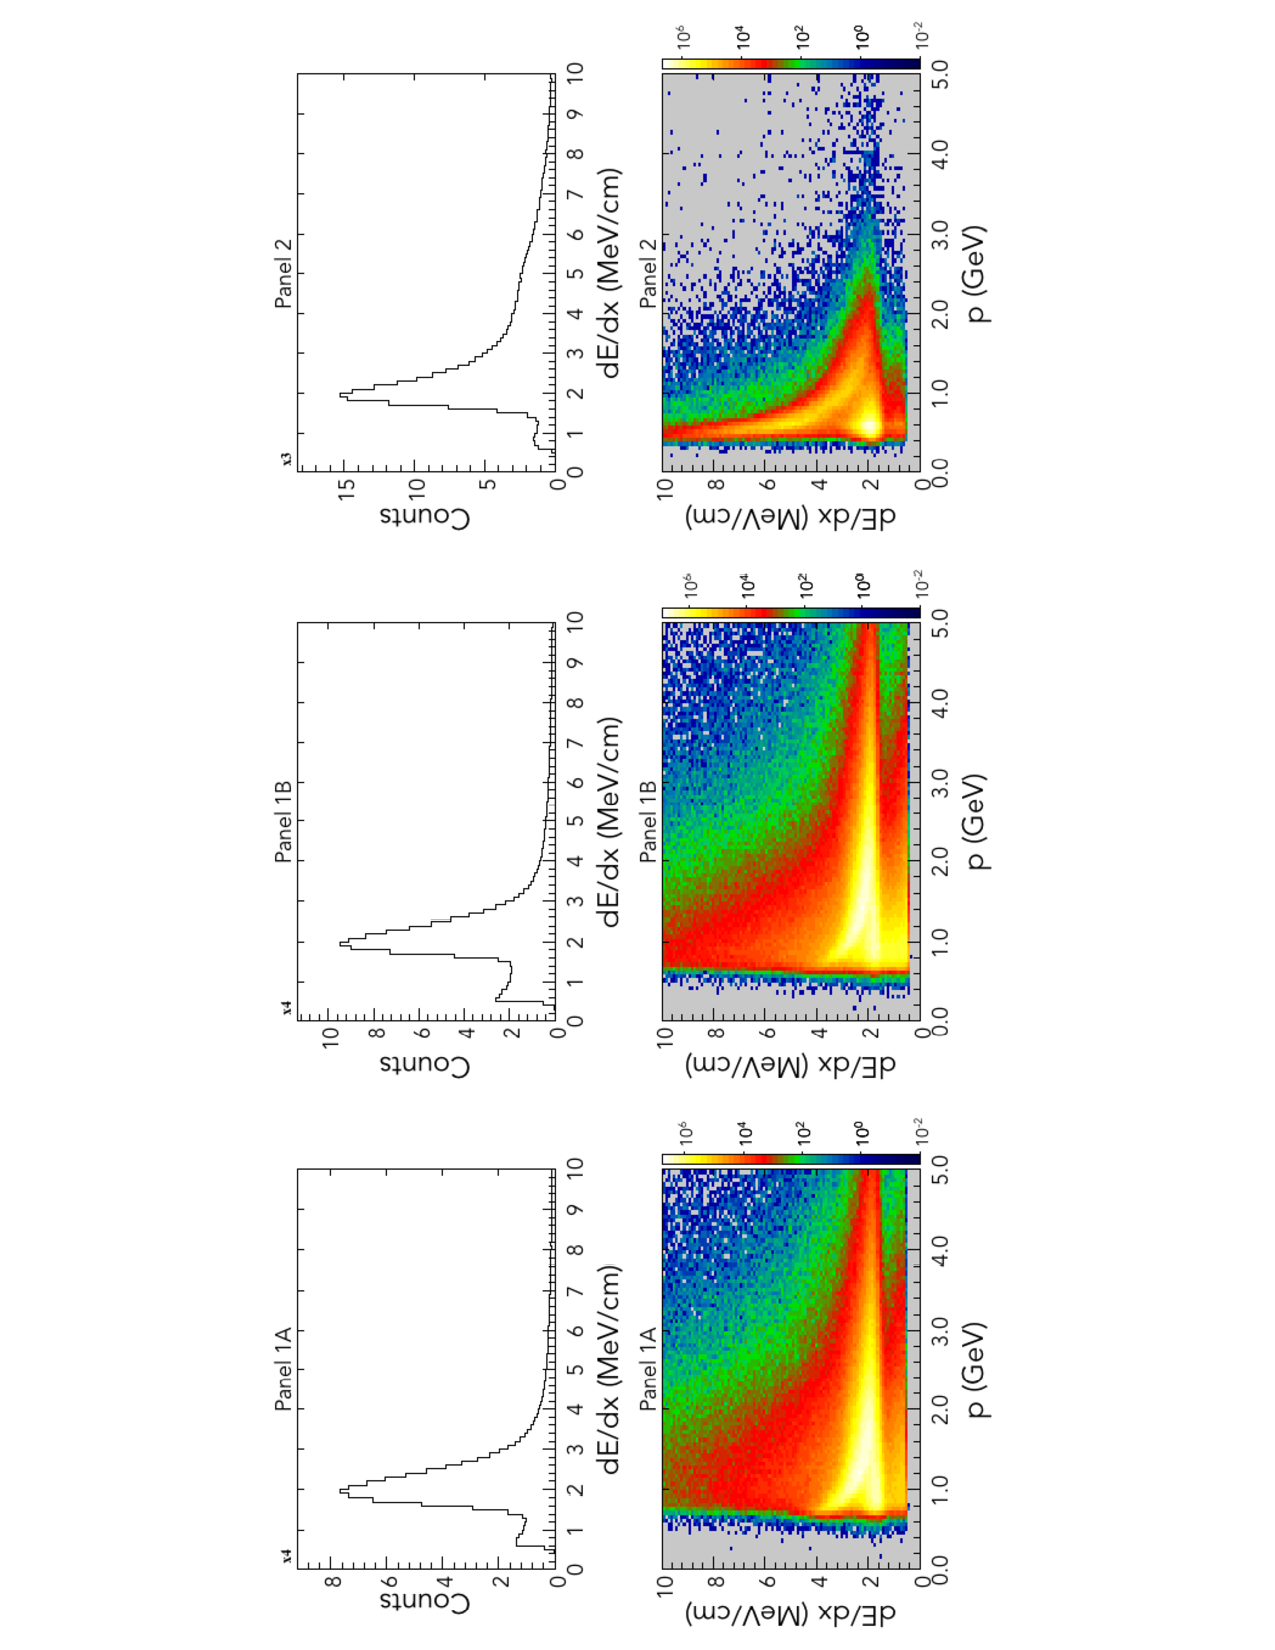
\includegraphics[width=0.9\textwidth,,height=0.50\textheight,natwidth=610,natheight=642,angle=-90]
{pics/ftof-dedx.pdf}}}
\end{picture} 
\caption{(Color Online) Measured FTOF counter energy loss for positively charged particles from 10.6~GeV
electrons incident on a liquid-hydrogen target normalized by the extrapolated path length from the projection
of the forward track through the counter array. This $dE/dx$ (MeV/cm) shows separation of minimum-ionizing
particles against more heavily ionizing particles summed over the counters in panel-1a (left), panel-1b (middle),
and panel-2 (left). The top row of plots show the measured $dE/dx$ and the bottom row of plots show $dE/dx$
vs. track momentum (GeV).}
\label{ftof-dedx}
\end{figure}
%%%%%%%%%%%%%%%%%%%%%%%%%%%%%%%%%%%%%%%%%%%%%%%%%%%%%%%%

\subsubsection{Attenuation Length Measurements}
\label{sec:attlen}

The attenuation length of the scintillation bars represents the distance $\lambda$ into the material
where the probability that the photon has been absorbed is $1/e$. The measured ADC values for each
PMT can be written in terms of the attenuation length as:

\begin{equation}
\label{al-adc}
ADC = A_0 e^{\pm x/\lambda},
\end{equation}

\noindent
where $A_0$ is a constant, $x$ is the distance along the counter with respect to the PMT location, and
$\lambda$ is the counter attenuation length. Forming this ratio from the ADC values from the left and
right ends of the counter,

\begin{equation}
\label{linear}
\log \left( \frac{(ADC-PED)_R}{(ADC-PED)_L} \right ) = C + \frac{2x}{\lambda}.
\end{equation}

\noindent
A linear fit of the ADC log ratio vs. coordinate can be used to extract the effective counter attenuation
length. 

Fig.~\ref{atten-len} shows the measured attenuation lengths for the FTOF counters in one sector of
the CLAS12 Forward Detector extracted from data with a 10.6~GeV electron beam incident on a
liquid-hydrogen target.

%%%%%%%%%%%%%%%%%%%%%%%%%%%%%%%%%%%%%%%%%%%%%%%%%%%%%%%%%
\begin{figure}[htbp]
\vspace{3.7cm}
\begin{picture}(30,50) 
\put(-5,-70)
{\hbox{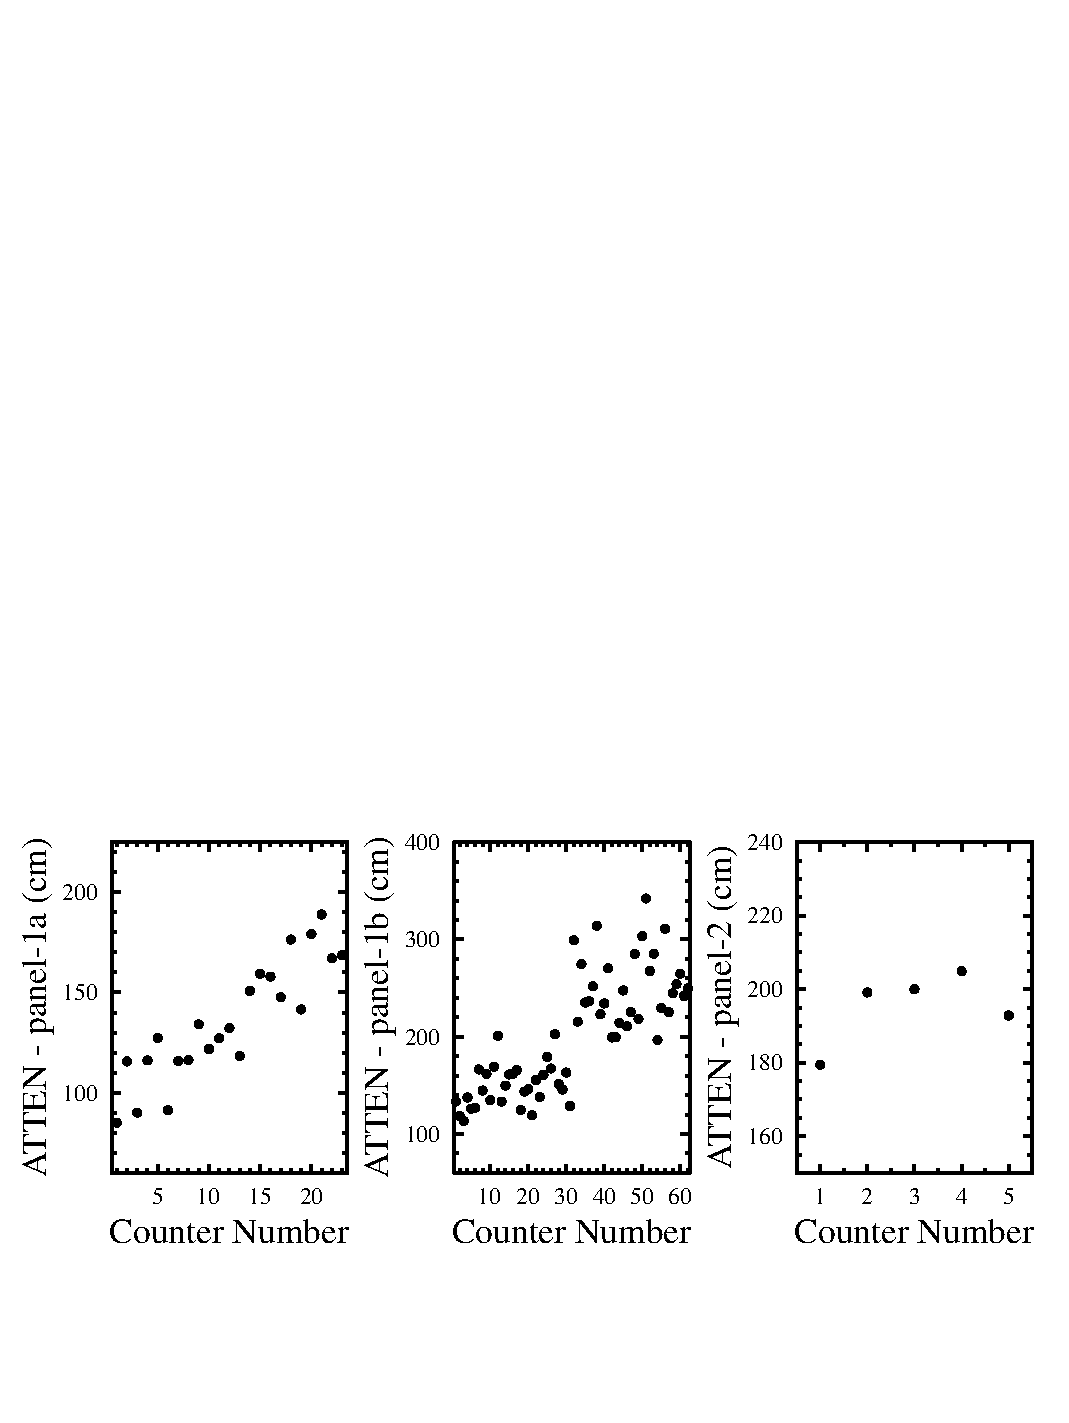
\includegraphics[width=1.2\textwidth,natwidth=610,natheight=642]{pics/atten-r4013.pdf}}}
\end{picture} 
\caption{Counter attenuation lengths (cm) vs. counter number for all FTOF counters in one sector of the
CLAS12 Forward Detector determined from beam data.}
\label{atten-len}
\end{figure}
%%%%%%%%%%%%%%%%%%%%%%%%%%%%%%%%%%%%%%%%%%%%%%%%%%%%%%%%%

\subsubsection{Effective Velocity Determination}
\label{sec:veff}

The effective velocity of light in each counter employs a calculation based comparing the reconstructed
coordinate information along the scintillation bar from the timing information and from the track hit
coordinate determined from extrapolation of the track beyond the drift chambers to the location of the
FTOF counters. Fig.~\ref{veff} shows the measured effective velocity for each counter in one sector of
the CLAS12 Forward Detector using data with a 10.6~GeV electron beam incident on a liquid-hydrogen
target. 

As the counter length increases, so does the effective velocity because light rays at large angles with longer
actual trajectories to the PMT are systematically lost owing to attenuation. These constants are used in FTOF
analysis to determine the hit time for each event from the measured TDC times. The intrinsic position
resolution is given by $v_{eff} \times \sigma(t_L - t_R)$ for each counter, which is most relevant for the
interactions of neutral particles. The position for charged particles can be measured more precisely with the
drift chambers.

%%%%%%%%%%%%%%%%%%%%%%%%%%%%%%%%%%%%%%%%%%%%%%%%%%%%%%%%%
\begin{figure}[htbp]
\vspace{3.7cm}
\begin{picture}(30,50) 
\put(-10,-70)
{\hbox{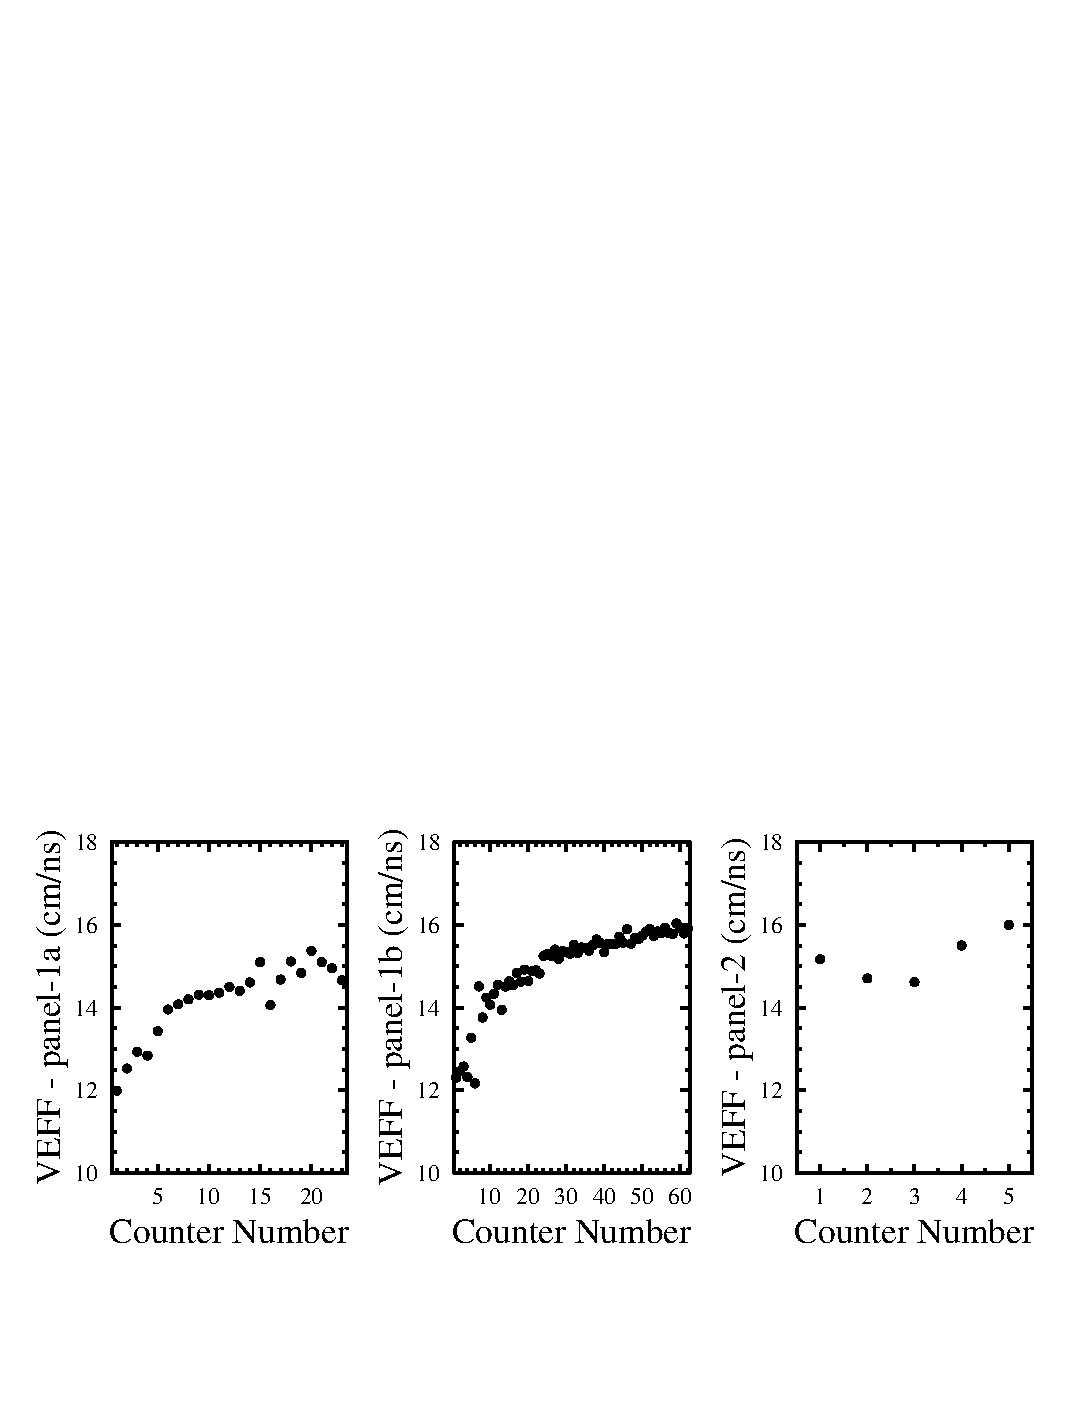
\includegraphics[width=1.2\textwidth,natwidth=610,natheight=642]{pics/veff-r4013.pdf}}}
\end{picture} 
\caption{Counter effective velocities (cm/ns) vs. counter number for all FTOF counters in one sector of
the CLAS12 Forward Carriage determined from beam data.}
\label{veff}
\end{figure}
%%%%%%%%%%%%%%%%%%%%%%%%%%%%%%%%%%%%%%%%%%%%%%%%%%%%%%%%%

\subsubsection{Time-Walk Corrections}
\label{sec-tw}

The approach that we adopted to correct the FTOF TDC times for time-walk effects is different than
was employed for our bench test studies of the counters in their cosmic ray test stands described in
Section~\ref{sec-bench}. We ultimately settled on an approach that first accounts for the average hit
position independent correction with a time-walk functional of the form:

\begin{equation}
\label{tw-func}
t^{corr}_{L,R} = t_{L,R} - \frac{tw0_{L,R}}{\sqrt{(ADC - PED)_{L,R}}}.
\end{equation}

The time-walk amplitude $A_0$ is determined by defining the following vertex time residual for each PMT:

\begin{equation}
\label{tres}
t_{L,R}^{res} = \left(t_{L,R} - \frac{d_{L,R}^{DC}}{v_{eff}} - \frac{L}{\beta c} \right) 
- \left( t_{RF} + \frac{z_{vert}}{\beta_e c} \right),
\end{equation}

\noindent
where $t_{L,R}$ are the measured TDC times after the left/right PMT time offset determination, 
$d^{DC}/v_{eff}$ corrects the time measured at the PMT to the time of the track hit point
on the counter determined from DC tracking information, $L/(\beta c)$ is the track flight time
from the reaction vertex to the FTOF. The track path length $L$ comes from DC tracking
and $\beta$ is determined from the FTOF timing and the DC path length, with the particle
identification determined from the Event Builder. The term $z_{vert}/(\beta_e c)$ is a term to
correct the RF time $t_{RF}$ to account for the actual electron beam event vertex location along
the $z$-axis of the extended target (hence the use of $\beta = \beta_e$)yy. In this expression,
$d_{L,R}^{DC}$ are the distances along the bar from the track hit point to the left and right PMTs.
This expression represents the FTOF hit time from a single PMT traced back to the reaction
vertex and compared to a precise time reference given by the RF signal from the accelerator.
As this $t_{RF}$ represents a reference time for the arrival of the electron beam bunch at a fixed
position along the beamline in Hall~B assigned as the center of the target, the time must be
corrected for the displacement of the reaction vertex along the length of the hydrogen target.

As the beam bucket that was associated with the event is not determined at this point, the 
time walk for each PMT is actually determined using the modulus of $t^{res}_{L,R}$ with the RF
beam bucket period $T_{RF}=$1/(RF frequency) by fitting:

\begin{equation}
t'_{L,R} = mod (t^{res}_{L,R}, T_{RF})~{\rm vs.}~(ADC-PED)_{L,R}.
\end{equation}

Fig.~\ref{twalk-plot} shows the $t'$ vs. $ADC$ distribution for a representative FTOF PMT in
panel-1b from beam data using a 10.6~GeV electron beam incident upon a liquid-hydrogen target.
Note that all distributions that employ $t'_{L,R}$ are sorted in 25~ps bins (consistent with the TDC
LSB). The overall scale of the time-walk effects spanning the full dynamic range of the ADC is
$\sim$2~ns.

%%%%%%%%%%%%%%%%%%%%%%%%%%%%%%%%%%%%%%%%%%%%%%%%%%%%%%%%%%
\begin{figure}[htbp]
\vspace{4.0cm}
\begin{picture}(50,50) 
\put(20,205)
{\hbox{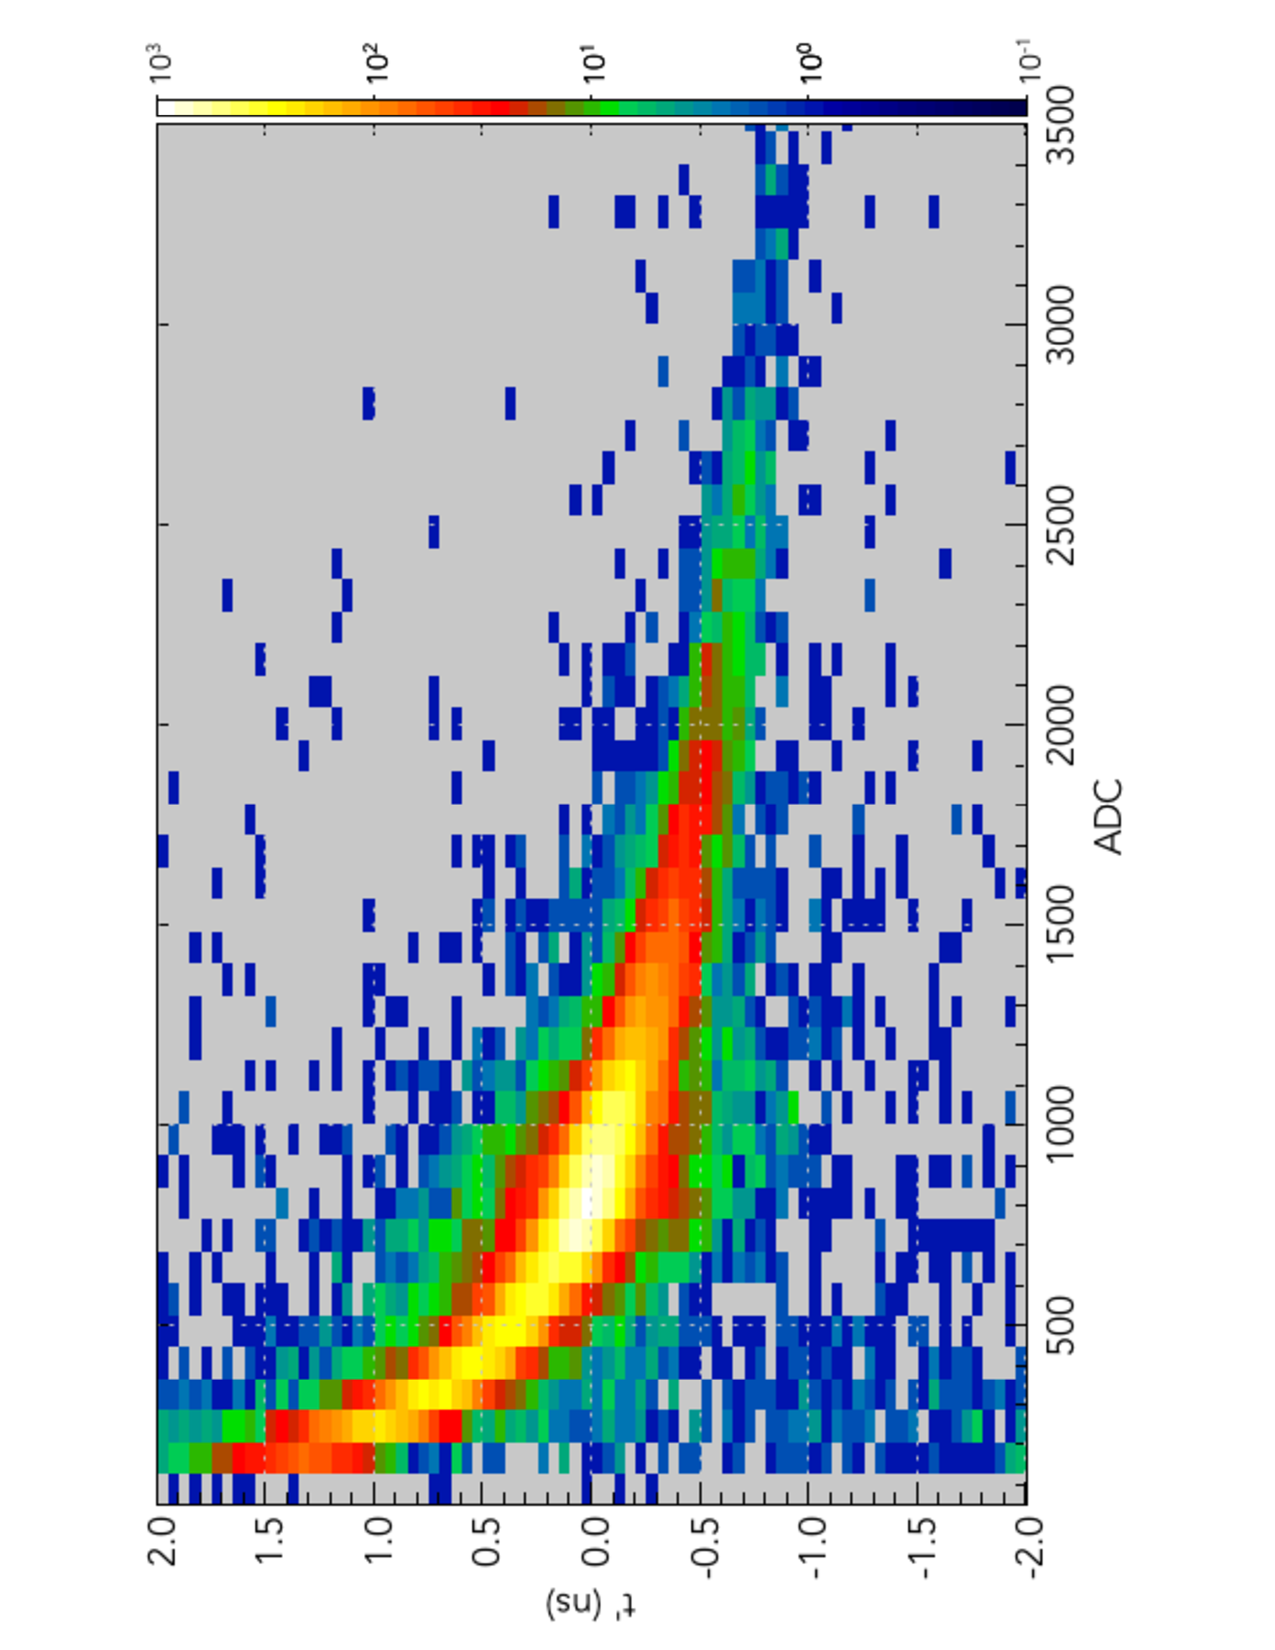
\includegraphics[width=0.65\textwidth,natwidth=610,natheight=642,angle=-90]{pics/twalk-plot.pdf}}}
\end{picture} 
\caption{(Color Online) Plot of $t'$ (ns) vs. $ADC$ for one representative PMT from panel-1b from beam
data. As $t'$ is defined using the modulus of $T_{RF}$, its limits span $\pm T_{RF}/2$.}
\label{twalk-plot}
\end{figure}
%%%%%%%%%%%%%%%%%%%%%%%%%%%%%%%%%%%%%%%%%%%%%%%%%%%%%%%%%%

The second part of the full time-walk correction accounts for the important position-dependence of the
effect as discussed in Section~\ref{sec-bench}. To simplify the algorithm the approach we take is to
determine the position-independent correction first for the left-side and the right-side counter PMTs.
In a second step we then fit a second-order polynomial to the counter hit time vs. hit position along the
counter. Fig.~\ref{twalk-pos} shows the distribution before and after the correction. The time employed
for this step is the track hit time at the vertex (relative to the vertex-corrected RF time) averaging the
left and right PMT hit times. The before distributions reveal a characteristic ``smile'' pattern after the
position-independent time-walk correction is made. This reflects the convolution of the unaccounted for
position-dependent time-walk effects on the measured times incorporating both the left and right PMTs
each with their own linearly falling time-walk amplitude moving away from the PMT as discussed in
Section~\ref{sec-bench}. Effectively this approach actually accounts for all remaining position dependence
in the calibration parameters. Specifically it should be the case that the effective velocity changes with
position along the bar moving away from the PMT. However, the dominant position-dependent parameter
accounted for here is the time-walk amplitude.

%%%%%%%%%%%%%%%%%%%%%%%%%%%%%%%%%%%%%%%%%%%%%%%%%%%%%%%%%%
\begin{figure}[htbp]
\vspace{2.7cm}
\begin{picture}(50,50) 
\put(-27,155)
{\hbox{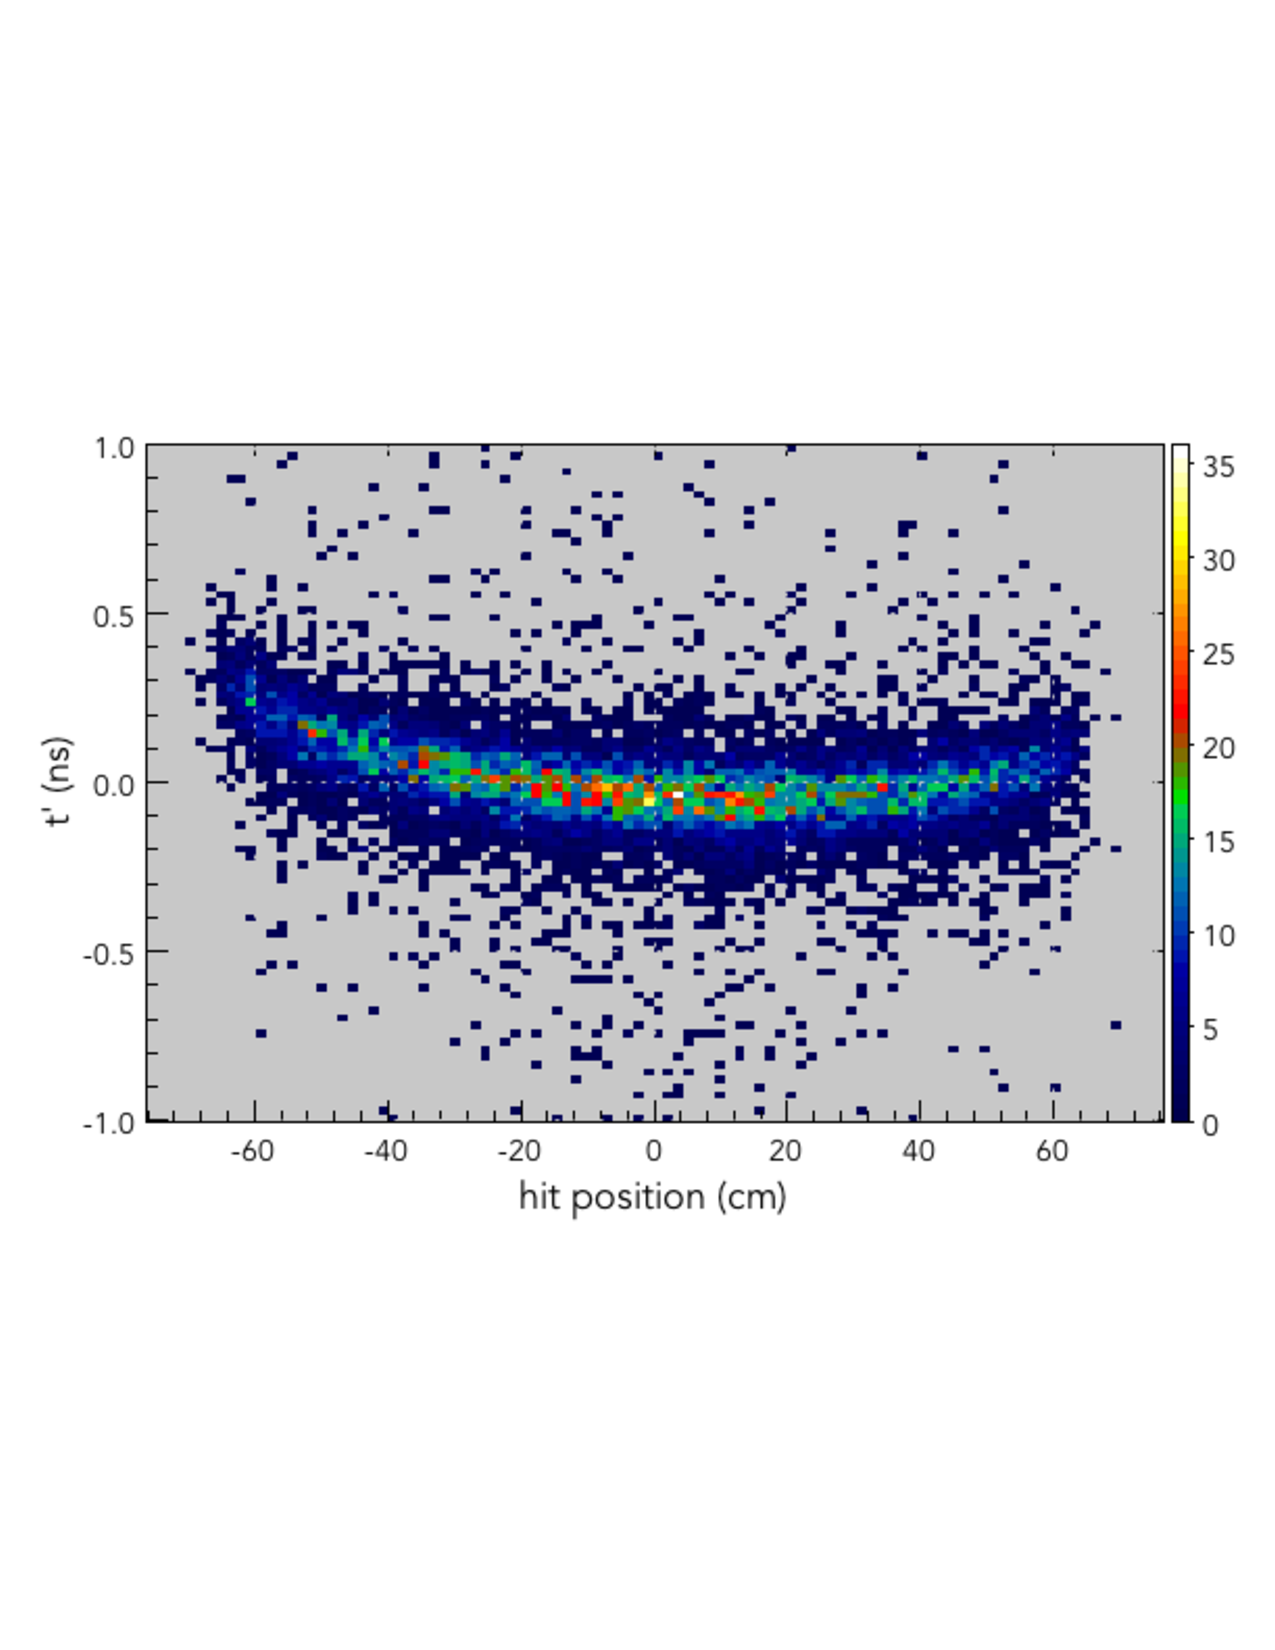
\includegraphics[width=0.50\textwidth,natwidth=610,natheight=642,angle=-90]{pics/p1b-posdep1.pdf}}}
\put(165,155)
{\hbox{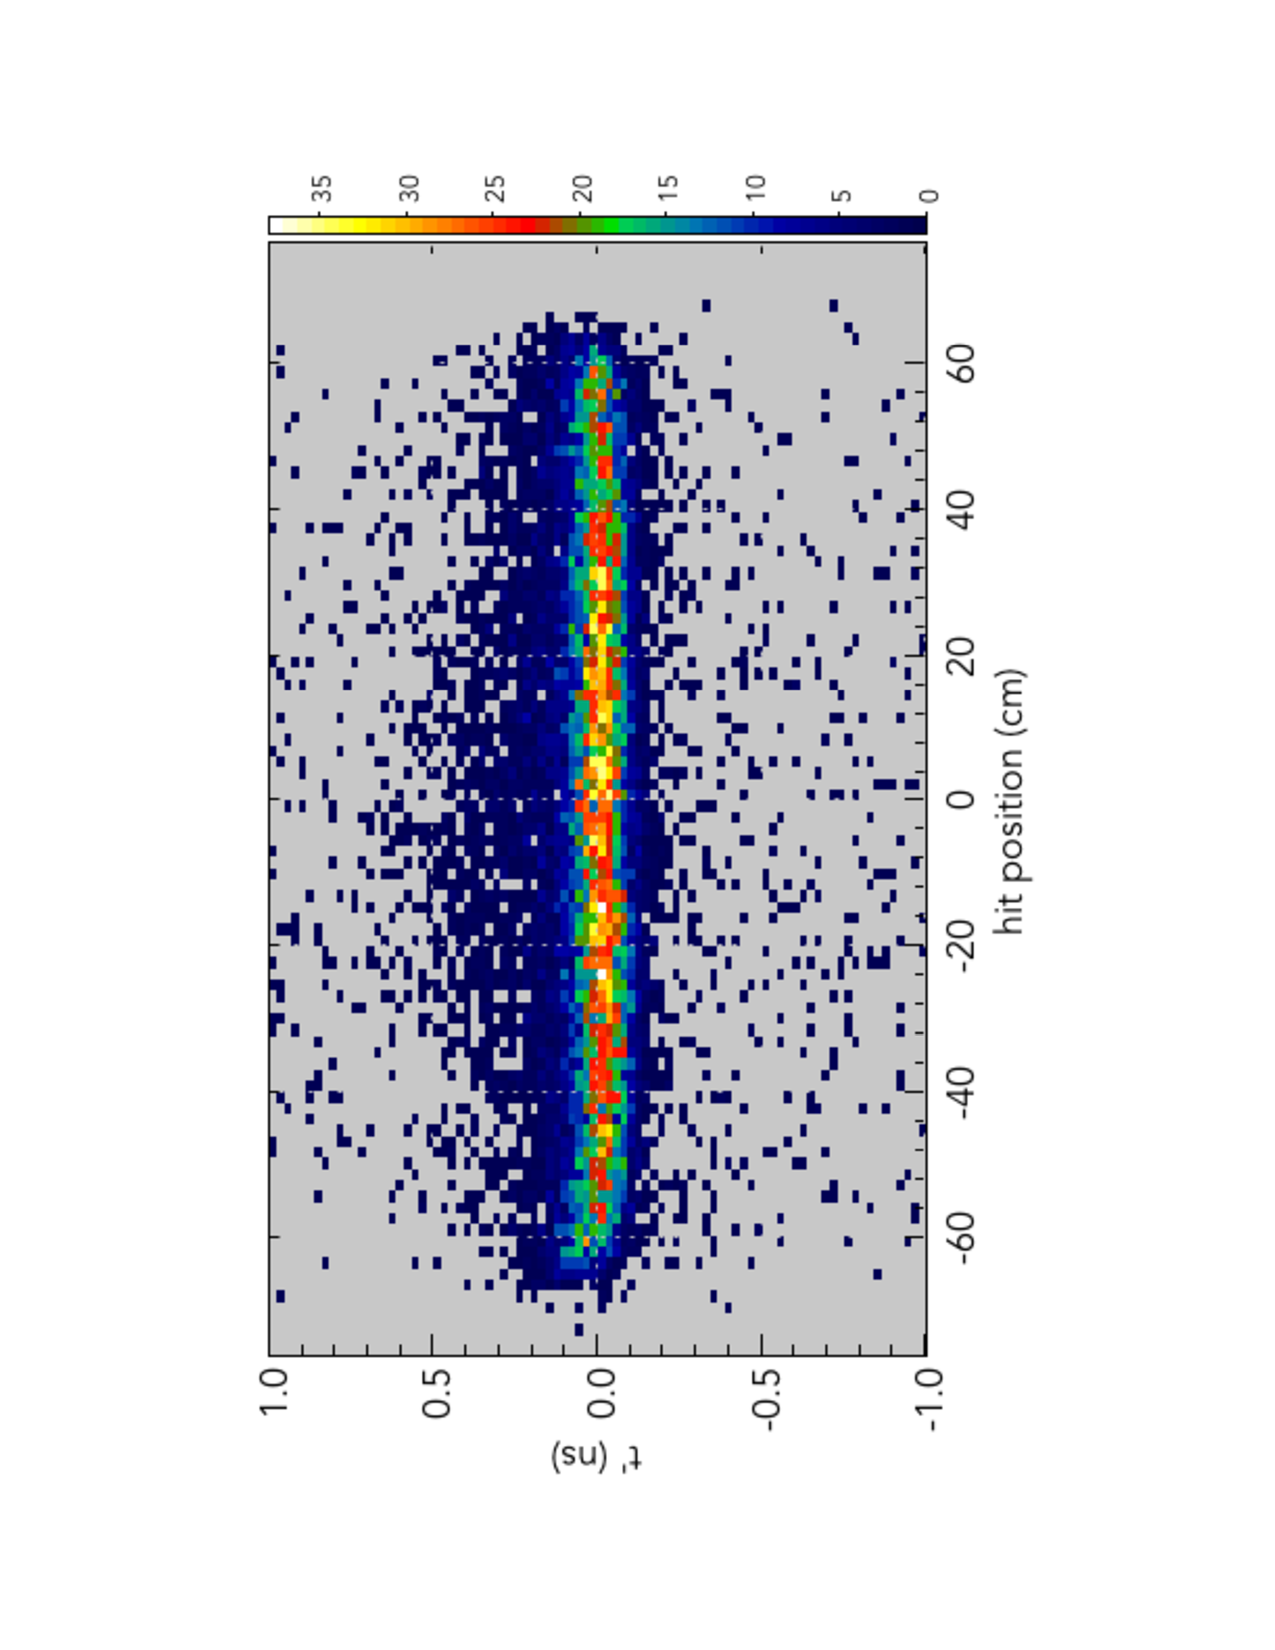
\includegraphics[width=0.50\textwidth,natwidth=610,natheight=642,angle=-90]{pics/p1b-posdep2.pdf}}}
\end{picture} 
\caption{(Color Online) Plot of $t'$ (ns) vs. hit position (cm) along the bar from beam data after the
position-independent time-walk correction (left) and after the ad hoc second-order polynomial fit to
remove the residual coordinate dependence (right).}
\label{twalk-pos}
\end{figure}
%%%%%%%%%%%%%%%%%%%%%%%%%%%%%%%%%%%%%%%%%%%%%%%%%%%%%%%%%%

\subsubsection{Counter-to-Counter Time Alignment}
\label{sec-talign}

The flight time of a charged particle from the reaction vertex to an FTOF counter is given by:

\begin{equation}
TOF = \overline{t}_{hit} - t_{ST},
\end{equation}

\noindent
where $\overline{t}_{hit}$ is the average FTOF counter hit time and $t_{ST}$ is the event start time.
The event start time is associated with the RF but needs to be synchronized with the particular RF
beam bucket associated with the event. The beam bunch width within the RF beam bucket is only
$\sim$2~ps and, therefore, represents a precise time marker. However, as the RF time signal has a
period of $T_{RF}$, it is not initially known which RF beam bucket was the one associated with the
event that led to the hits in the FTOF counter.

The determination of the absolute flight time of charged particle tracks from the reaction vertex
to the FTOF counters is performed in two steps. In the first step, fine timing offsets (binned in the
LSB of the TDCs = 25~ps) are determined to align the FTOF hit times traced back to the vertex for
each counter within the RF time window. In the second step, coarse timing offsets binned in units of the
RF period $T_{RF}$ are determined to fix the specific RF beam bucket associated with the event.

The fine timing alignment algorithm uses the FTOF hit time traced to the event vertex relative to the RF
to align the vertex times of all FTOF hits (modulo $T_{RF}$). However, instead of using the separate
left and right PMT hit times as in Eq.(\ref{tres}), this algorithm uses the average counter hit times, 

\begin{equation}
t_{res}' = mod \left[ \left( \left(\overline{t}_{hit} - \frac{L}{\beta c} \right) -
\left(t_{RF} + \frac{z_{vert}}{\beta_e c} \right) \right), T_{RF} \right].
\end{equation}

Fig.~\ref{rfp-plot} shows the $t_{res}'$ distribution for one representative FTOF counter. The centroid
of the Gaussian fit gives the fine timing offset. The width of the Gaussian fit represents a measure of the
effective timing resolution of the counter. To display the full $t_{res}'$ distribution avoiding any
wrap-around effects near the edges of the $T_{RF}$ range, the algorithm plots the $t_{res}'$ distribution
in a range of $\pm T_{RF}/2$ about the peak channel in the distribution.

%%%%%%%%%%%%%%%%%%%%%%%%%%%%%%%%%%%%%%%%%%%%%%%%%%%%%%%%%%
\begin{figure}[htbp]
\vspace{4.0cm}
\begin{picture}(50,50) 
\put(30,205)
{\hbox{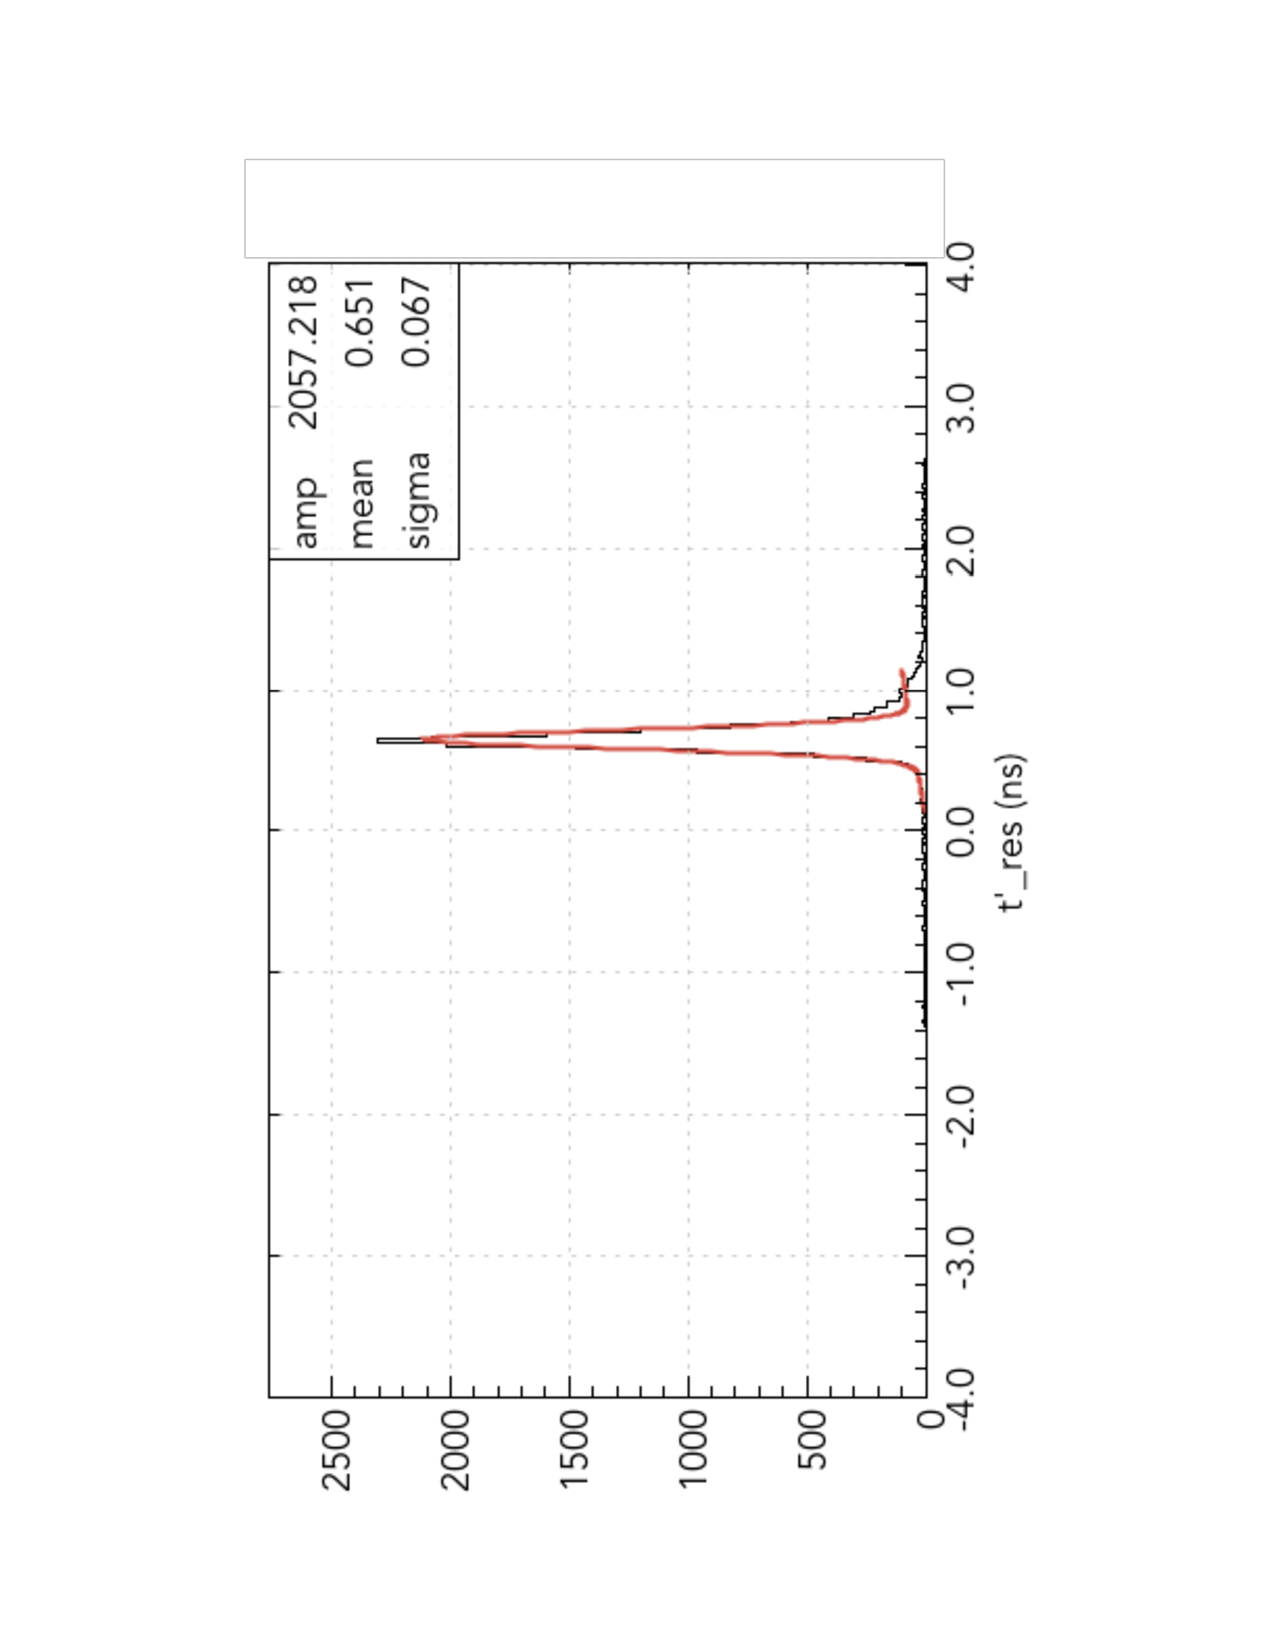
\includegraphics[width=0.65\textwidth,natwidth=610,natheight=642,angle=-90]{pics/rfp-plot.pdf}}}
\end{picture} 
\caption{(Color Online) Distribution of the FTOF hit times from beam data traced back to the vertex relative
to the RF (ns) for one representative FTOF panel-1b counter with the Gaussian plus background fit overlaid
to determine the counter RF offset and the effective counter timing resolution. As $t'$ is defined using the
modulus of $T_{RF}$ this distribution is limited to span $\pm T_{RF}$.}
\label{rfp-plot}
\end{figure}
%%%%%%%%%%%%%%%%%%%%%%%%%%%%%%%%%%%%%%%%%%%%%%%%%%%%%%%%%%

After the fine timing offset calibration, the counter timing is precisely aligned modulo $T_{RF}$. The next
step in the FTOF timing calibration is to fix the measured hit times for all counters to the specific RF bunch
associated with the event.  This is carried out using coincidences of charged particle tracks to link the hit
times of all counters across the full FTOF system.

The coarse timing offset algorithm (called P2P for paddle-to-paddle) selects events with two forward-going
charged tracks and for each FTOF counter computes the vertex time difference for a given FTOF counter
relative to hits in all of the other FTOF counters,

\begin{equation}
t_{P2P} = t_{vert}^1 - t_{vert}^2,
\end{equation}

\noindent
where,

\begin{equation}
t_{vert}^i = \overline{t}_{hit}^i - \frac{L}{\beta c}.
\end{equation}

At this point the counter times have already been aligned to within a multiple of $T_{RF}$. Note that
particle identification of each track is given by the Event Builder, and as both tracks are assumed to
originate from the same reaction vertex, no vertex time corrections are necessary. The algorithm
adjusts the vertex time differences over all counters to set them to zero. The coarse time offsets
represents a single parameter for each counter that is restricted to values of $n \cdot T_{RF}$, with
$n = 0, \pm 1, \pm 2, ...$.

Fig.~\ref{p2p-plot} shows the $t_{P2P}$ distribution for one representative FTOF counter before and
after the coarse timing alignment. As expected, the histogram is dominated by events in a single channel
(of width $T_{RF}$) centered about $T_{RF} = 0$. As these constants are predominantly determined by the
fixed system cable lengths, of which there are four different lengths used to connect the panel-1a and the
panel-1b counters, the constants primarily reflect the differences in the signal propagation times along
the signal cables. Note that the algorithm specifically identifies two track events for the calibration and
does not consider hits in panel-1b and panel-1a associated with the same track.

%%%%%%%%%%%%%%%%%%%%%%%%%%%%%%%%%%%%%%%%%%%%%%%%%%%%%%%%%%
\begin{figure}[htbp]
\vspace{2.7cm}
\begin{picture}(50,50) 
\put(-2,-70)
{\hbox{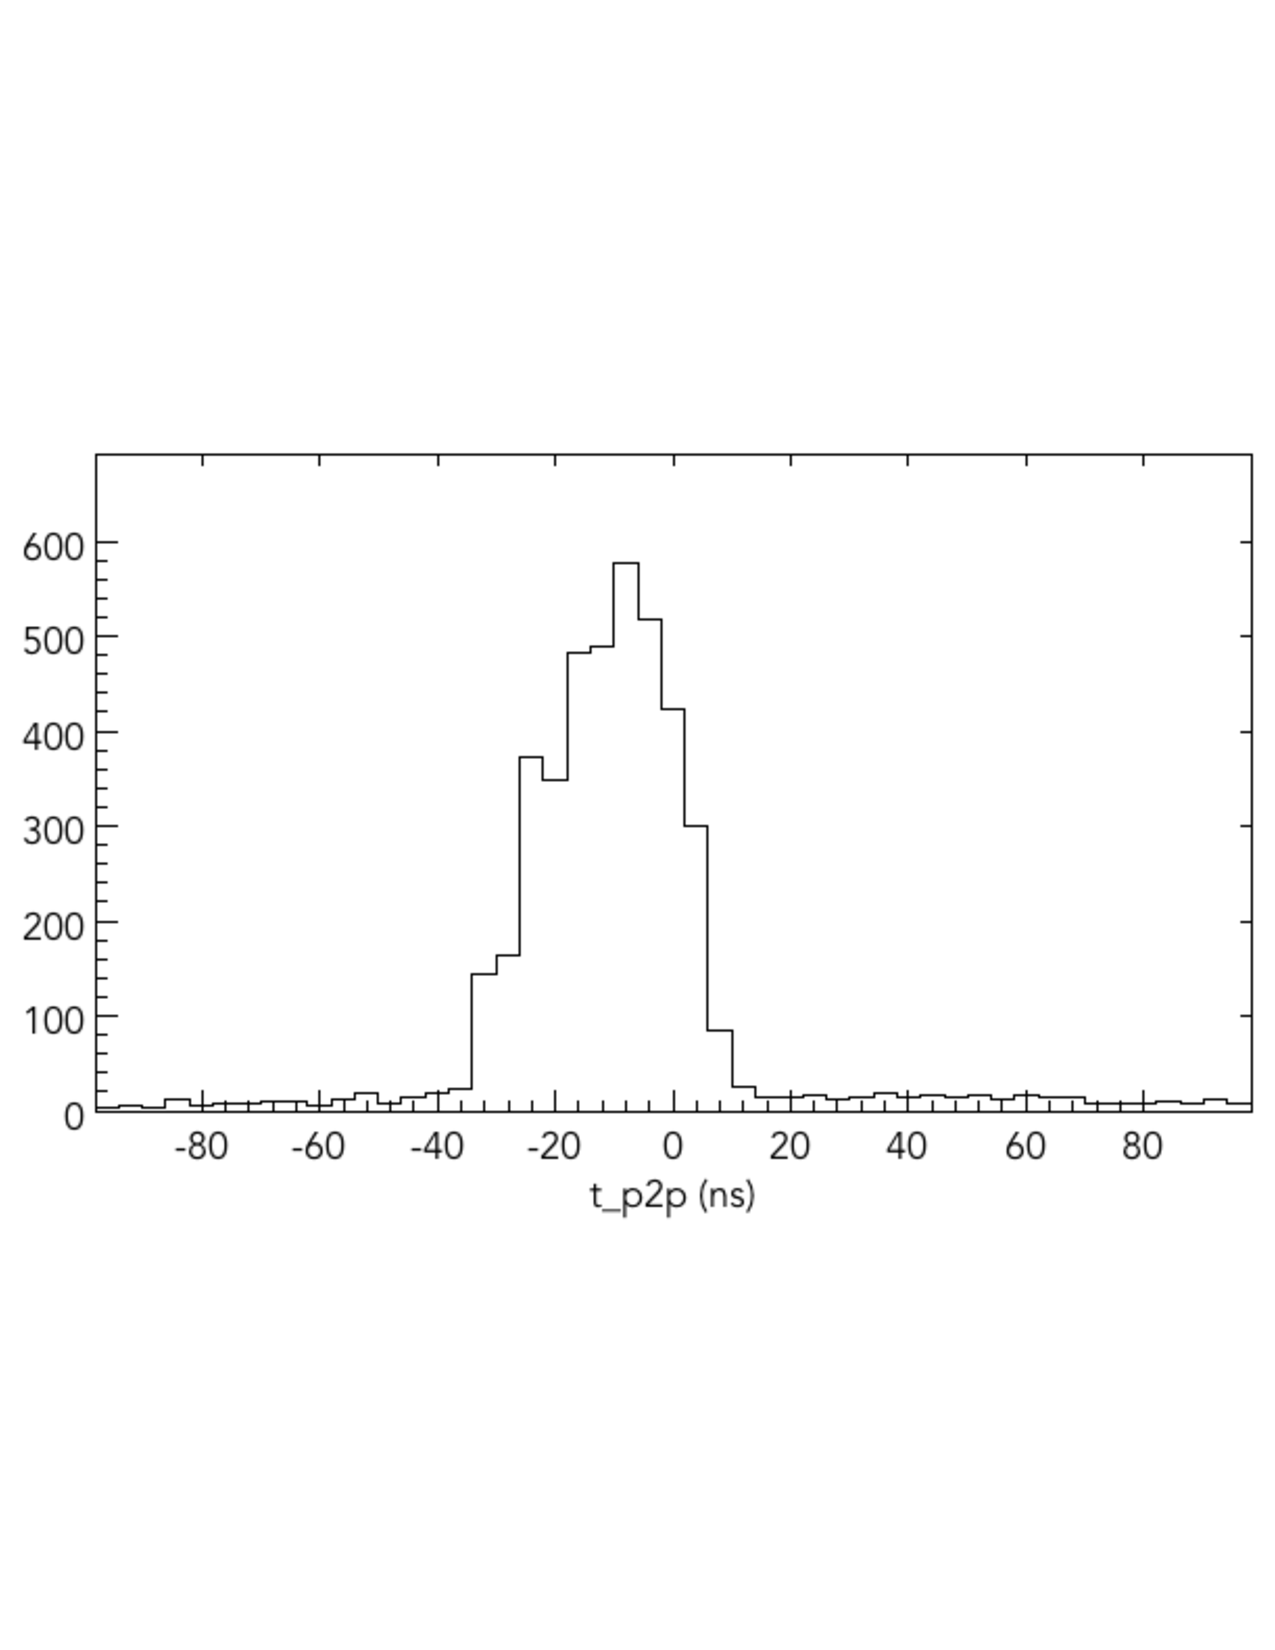
\includegraphics[width=0.50\textwidth,natwidth=610,natheight=642]{pics/p2p-plot1.pdf}}}
\put(197,-70)
{\hbox{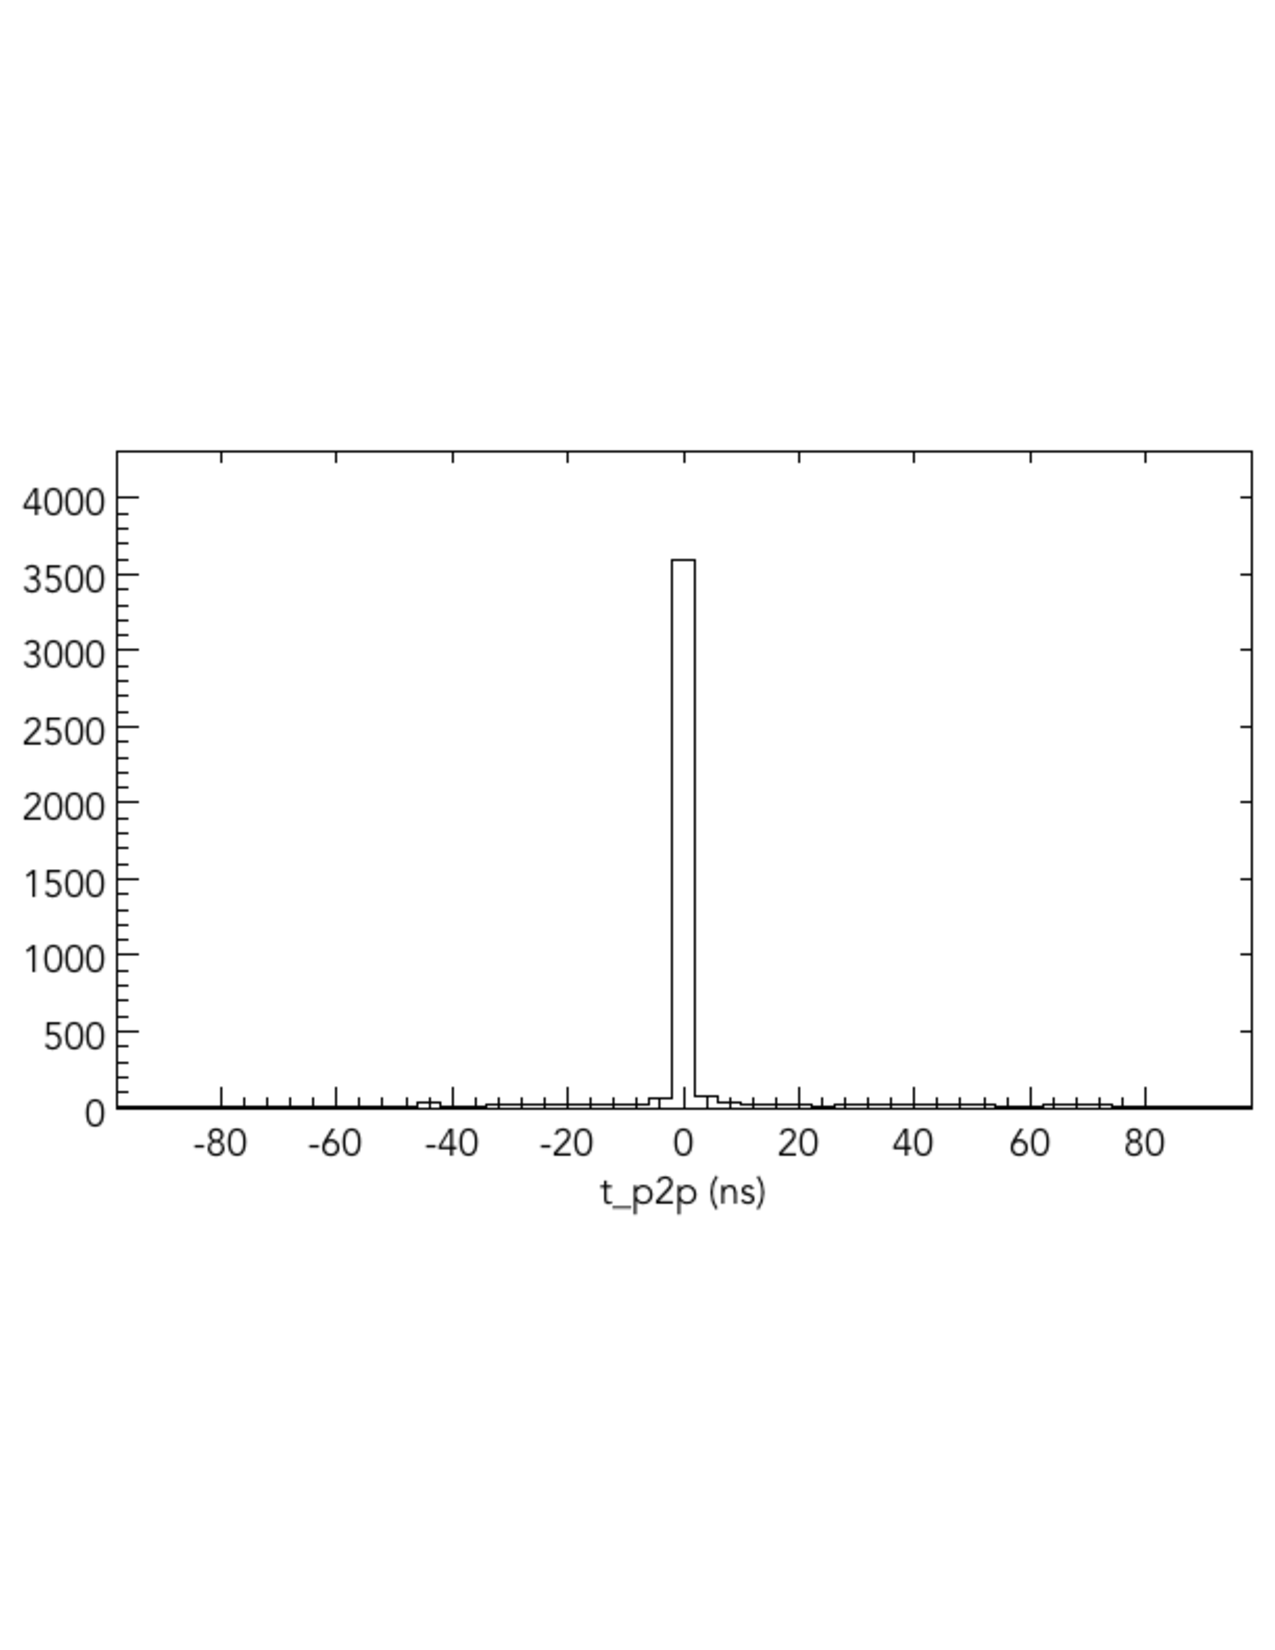
\includegraphics[width=0.50\textwidth,natwidth=610,natheight=642]{pics/p2p-plot2.pdf}}}
\end{picture} 
\caption{Distribution of the vertex time differences (ns) for tracks in a single representative FTOF
counter compared to tracks in all other FTOF counters using event samples with two forward-going
charged particle tracks. (Left) Before P2P corrections, (right) After P2P corrections. The histogram
is sorted in bins of $T_{RF}$.}
\label{p2p-plot}
\end{figure}
%%%%%%%%%%%%%%%%%%%%%%%%%%%%%%%%%%%%%%%%%%%%%%%%%%%%%%%%%%

\subsubsection{TDC Calibration}
\label{sec-tdccal}

The final calibration step is the calibration of the TDCs. This calibration is a single constant for each
TDC channel in the system that converts the measured TDC channel bin into time. The nominal TDC
LSB is 25~ps for the CAEN VX1290A and V1190A TDC units employed for the FTOF readout (see
Section~\ref{sec-elec}).

The calibration is completed by fitting the PMT time residuals of Eq.(\ref{tres}) vs. TDC channel using
a linear function. The TDC calibration is the value that fixes the slope of $t_{res}'$ to be zero.
Fig.~\ref{tdc-plot} shows the distribution of $t_{res}'$ vs. TDC for a representative FTOF counter.
Any bin-to-bin $\Delta t$ variations reflect remaining integral non-linearities in the measured TDC
compensation tables (see Section~\ref{sec-elec}). At the present time a single conversion constant
of 23.45~ps/channel is employed for the FTOF system TDCs.

%%%%%%%%%%%%%%%%%%%%%%%%%%%%%%%%%%%%%%%%%%%%%%%%%%%%%%%%%%
\begin{figure}[htbp]
\vspace{3.7cm}
\begin{picture}(50,50) 
\put(55,-95)
{\hbox{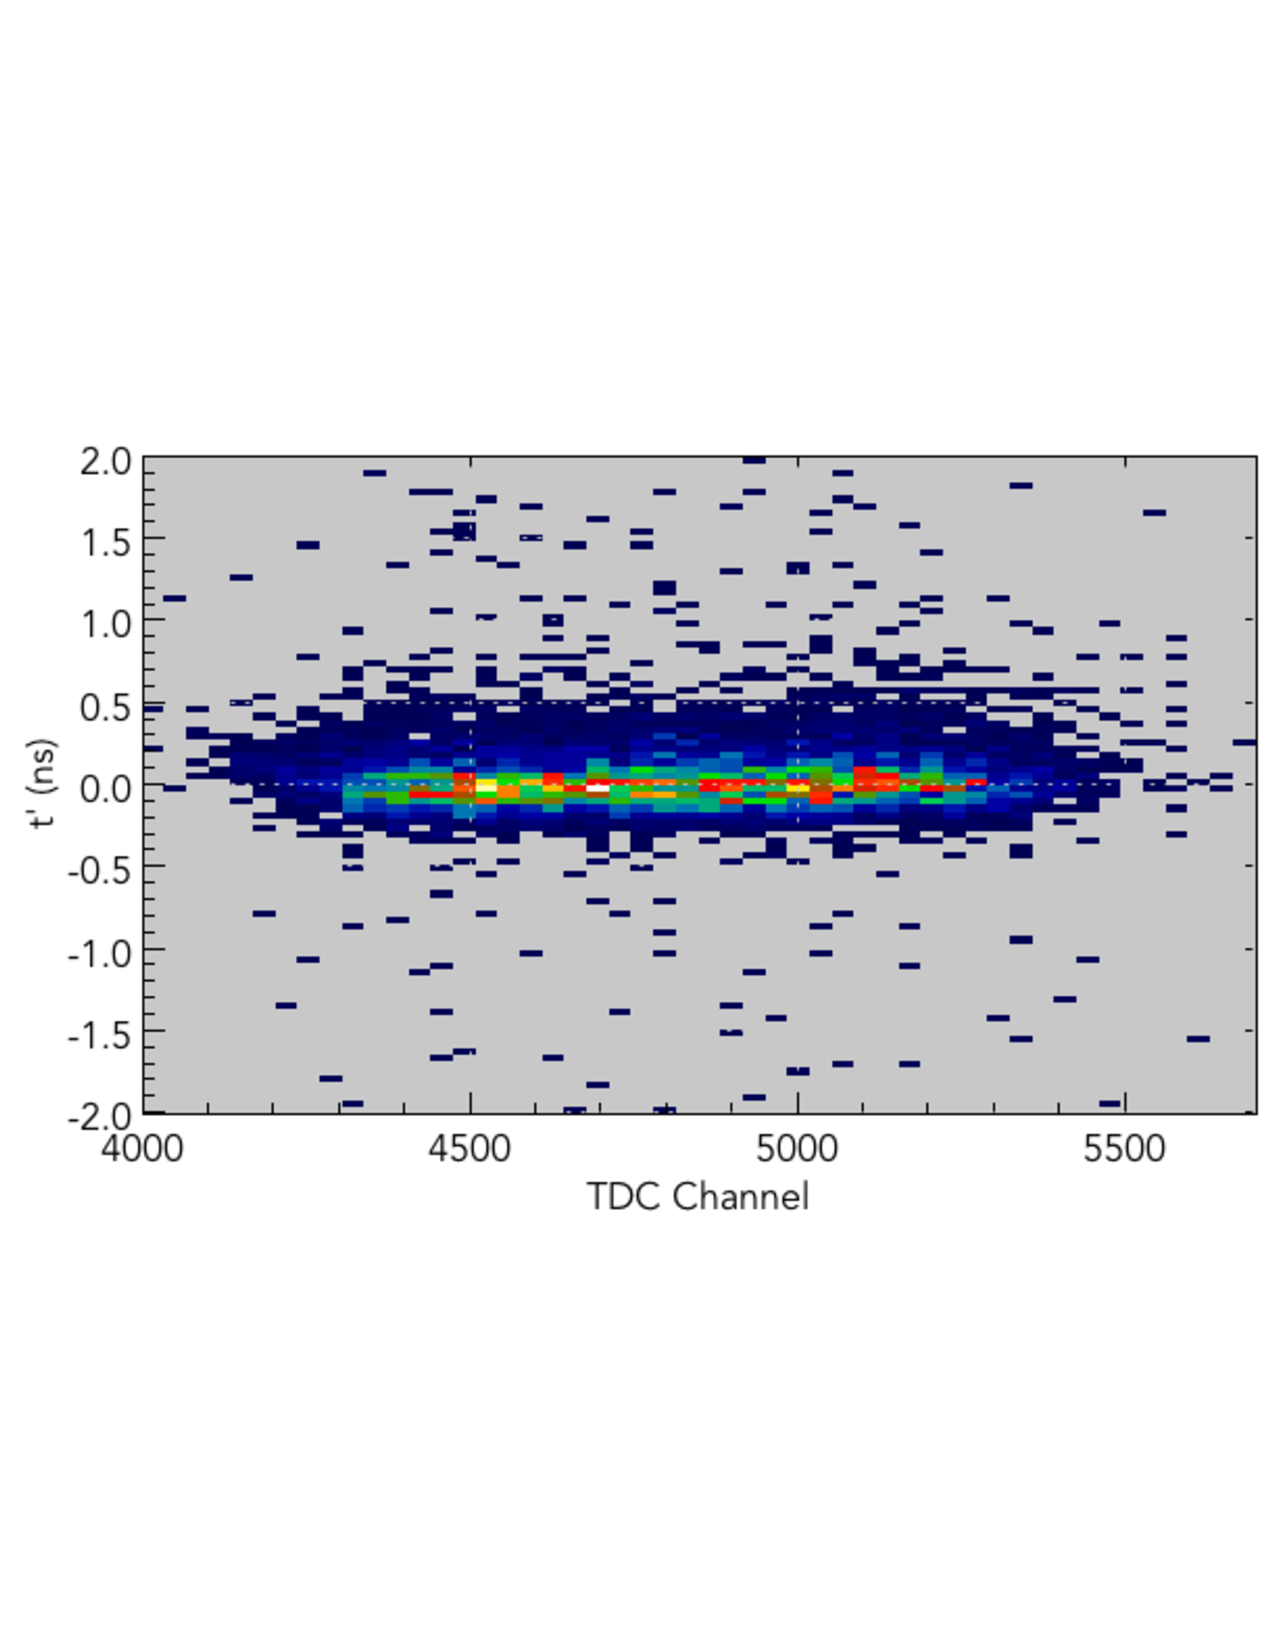
\includegraphics[width=0.65\textwidth,natwidth=610,natheight=642]{pics/tdc-plot.pdf}}}
\end{picture} 
\caption{(Color Online) Distribution of $t_{res}'$ (ns) vs. TDC channel for one representative 
FTOF panel-1b PMT. The TDC conversion constant for each channel is that which forces the slope of a linear
fit to be zero.}
\label{tdc-plot}
\end{figure}
%%%%%%%%%%%%%%%%%%%%%%%%%%%%%%%%%%%%%%%%%%%%%%%%%%%%%%%%%%

The CAEN TDCs used for the FTOF are readout with a 24~ns clock strobed so that all TDC times are
referenced to an edge of this clock. The CLAS12 trigger comes on the edge of a clock with a period of
4~ns and the TDC stop will not occur until the next 24~ns clock edge. The use of these two different
clocks introduces a delay between the trigger and the TDC stop given by $n \cdot 4$~ns, with
$n = 0 \to 5$ (referred to as the six-fold TDC cycle ambiguity) where $n$ is the phase. A TDC jitter
correction is made to define the value of the phase $n$ that is valid for the entire data run.

The average hit time resolution for the FTOF from the TDCs is $\sim$80~ps and that from the FTOF
FADCs given the rapid fall time of the fast PMT signals that provide for only 2-3 samples on the falling
edge is only $\sim$1~ns. A matching requirement of 10~ns between the TDC time and the FADC time is
employed during event reconstruction. While this matching requirement still needs to be tuned further,
at the current time is reasonably efficient at allowing the FADC hits to be matched with the TDC hits.
This is important as due to the different thresholds on the discriminators and the FADCs, the number
of entries in the hits lists are up to a factor of two different. The matching criteria is also essential
in order to assign the correct ADC information to the hit not only for the time-walk correction that
directly uses the measured ADC but also for the energy loss computation.

\subsubsection{Counter Time Resolutions}
\label{tres-beam}

The effective time resolutions for each counter determined during the fine timing alignment step
discussed in Section~\ref{sec-talign} are shown in Fig.~\ref{eff-tres}. These measurements were
taken after complete calibrations of the FTOF system from a beam data run with 10.6~GeV electrons
incident on a liquid-hydrogen target. The time resolution displayed here represents the quality of the
overall CLAS12 calibrations at the current time. The results are based on calibration procedures that
are not yet fully optimized, as well as uncertainties in the reconstructed momentum and path length
from the forward track reconstruction. Note that the time resolution floor-term $\sigma_0$ discussed
in Section~\ref{res-sec} and Eq.(\ref{timing-func}) does not include the contributions from the
reconstructed path length uncertainties. These uncertainties are polar and azimuthal angle dependent.
Near the torus coils the true magnetic field has different variations than accounted for in our conductor
model used to generate the field for the event reconstruction. As well, the path length uncertainties grow
strongly for high momentum tracks at small angles, which represent the dominant part of our kinematic
phase space at 10.6~GeV. It is also important to mention that studies of the CLAS12 subsystem detector
alignment based on survey data and based on zero-field straight track data are in progress. Misalignments of
the detector affect the quality and accuracy of the reconstruction. When these are accounted for their
contribution to the floor-term of the resolution function is reduced.

Nevertheless the time resolutions already achieved meet the system design specifications outlined in
Section~\ref{sec:overview} and shown in Table~\ref{spec-table}. With these resolutions, the quality of the
particle identification in the Forward Detector of CLAS12 allows the experimental program in Hall~B to reach
its goals. As further operating experience with CLAS12 is gained, we expect to realize further modest but
important improvements in the FTOF timing resolution that will allow $\pi/K$, $\pi/p$, and $K/p$ separation
in the Forward Detector of CLAS12 to be pushed to higher momenta than currently seen.

%%%%%%%%%%%%%%%%%%%%%%%%%%%%%%%%%%%%%%%%%%%%%%%%%%%%%%%%%
\begin{figure}[htbp]
\vspace{3.6cm}
\begin{picture}(50,50) 
\put(-5,-70)
{\hbox{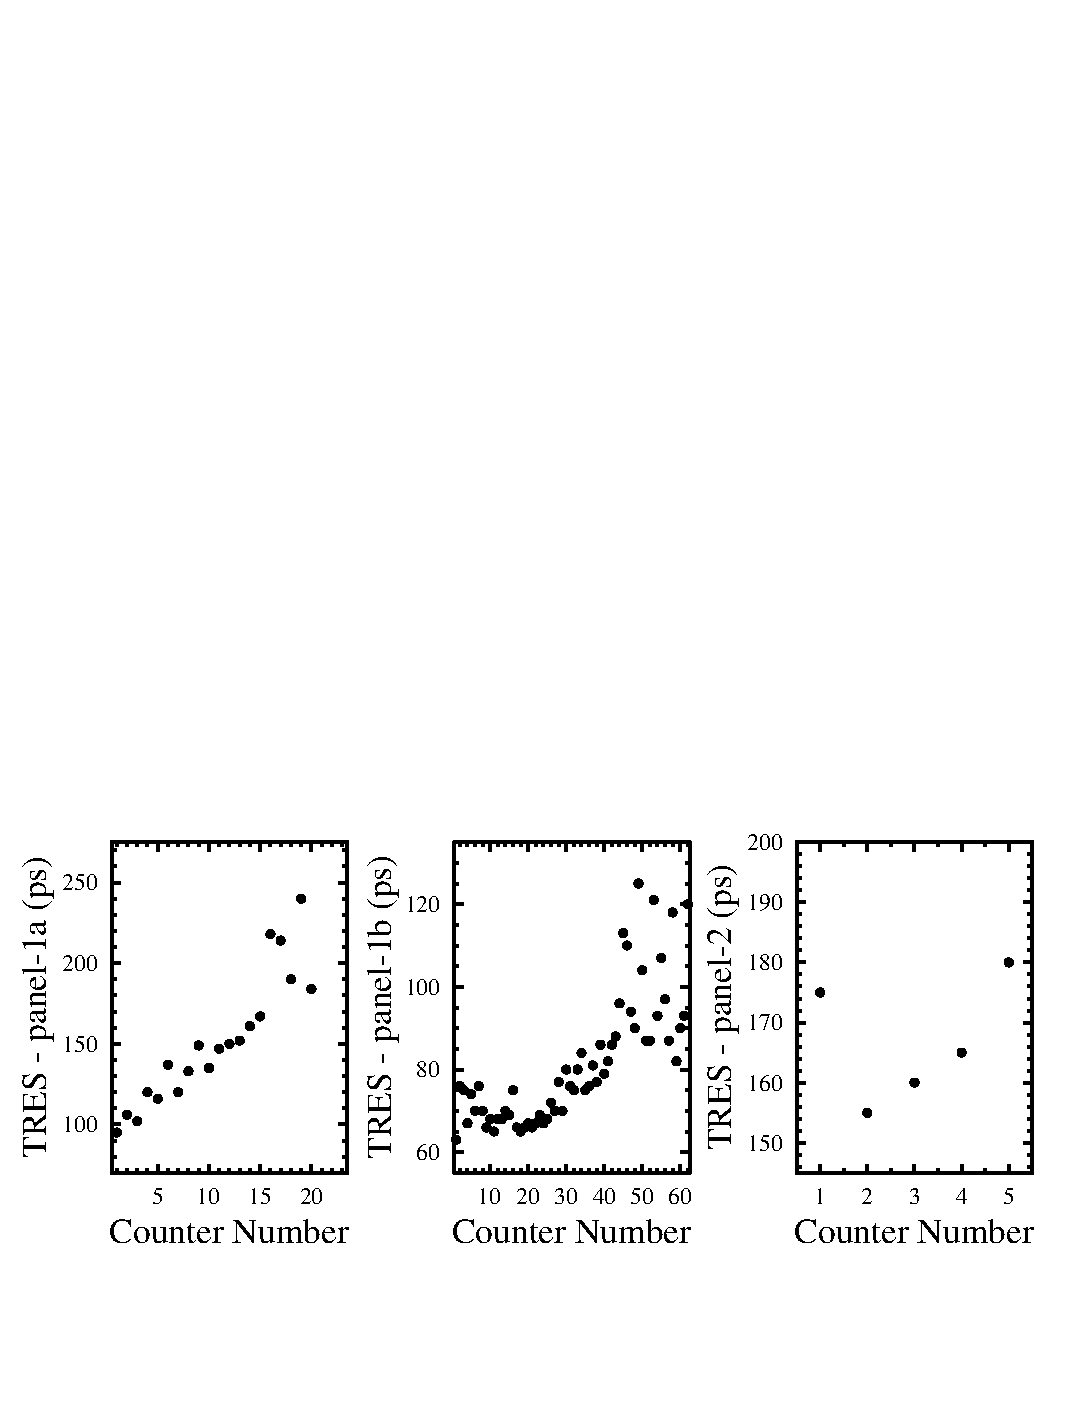
\includegraphics[width=1.2\textwidth,natwidth=610,natheight=642]{pics/res-r4013.pdf}}}
\end{picture} 
\caption{The measured effective time resolution (ps) vs. counter number for each of the FTOF counters
in sector~1 as determined using final state leptons and pions.}
\label{eff-tres}
\end{figure}
%%%%%%%%%%%%%%%%%%%%%%%%%%%%%%%%%%%%%%%%%%%%%%%%%%%%%%%%%

\subsubsection{Hit Clusterization and Hit Times}
\label{cluster}

The reconstructed FTOF counter hit times need to account for the time delays along the readout
path that include the PMT and voltage divider signal transit times, the signal propagation times along
the signal cables and the electronics, and the time-walk effects associated with the use of leading edge
discriminators for the readout. Full details on the FTOF reconstruction in terms of reconstructed hit
times and energy, the reconstruction algorithm, the time, energy, and coordinate uncertainties, and
the hit clustering and matching algorithms are provided in Ref.~\cite{ftof-recon}.

The track hit times reconstructed from the readout of the left and right PMTs are given by:

\begin{equation}
t_{L,R} = (C_{TDC} \cdot TDC_{L,R}) - t_{L,R}^{walk} \mp \frac{C_{LR}}{2} + C_{RF} + C_{p2p},
\end{equation}

\noindent
where $C_{TDC}$ is the TDC channel to time conversion factor, $TDC$ is the measured TDC value relative
to the trigger signal, $t^{walk}$ is the time-walk correction, $C_{LR}$ is the time shift to center the TDC
difference distribution relative to the track coordinate about 0, and $C_{RF}$ and $C_{p2p}$ are the time
shifts to align all of the counter times with respect to the RF and to each other, respectively.

The hit times of the passing charged particle relative to the trigger signal can be determined separately 
from the times $t_L$ and $t_R$ measured by the left and right PMTs, respectively, and are given by:

\begin{equation}
t_{hit}^{L,R} = t_{L,R} - \frac{d^{DC}_{L,R}}{v_{eff}}.
\end{equation}

\noindent
where $d^{DC}_{L,R}$ are the distances from the track hit point along the bar relative to the end of the
bar as determined by the drift chamber tracking information. The average FTOF hit time is then given by:

\begin{equation}
\bar{t}_{hit} = \frac{1}{2} ( t_{hit}^L + t_{hit}^R ) = \frac{1}{2} \left[ t_L + t_R - \frac{L}{v_{eff}} \right].
\end{equation}

Particle trajectories from the target passing through the plane of a given counter array (i.e. panel-1a,
panel-1b, or panel-2) can pass through up to two adjacent counters. To determine the full deposited
energy in a given counter layer, a clusterization algorithm is used to match the FTOF counter hits with
the track trajectory at the location of the FTOF array. Neighboring FTOF hits that match to the trajectory
are assigned to be part of a cluster. The assigned cluster energy is then the sum of the deposited energy
in both counters,

\begin{equation}
  E_{cluster} = \sum_{i=1}^{2} E_{dep}^i.
\end{equation}

\noindent
The relevant path length through the layer is then determined from ray tracing of the drift chamber track.
This path length through the layer is then used to compute $dE/dx$.

The hit time associated with the cluster in a given layer is based on an energy deposition weighted average
accounting for the time offset between the cluster hits. For the FTOF reconstruction the assigned hit
position in the counter is based on ray tracing of the charged track through the FTOF array. For each counter
the hit position is assigned as mid-way between the track entrance point and exit point on the bar. In this way
a cluster hit time is computed as:

\begin{equation}
t_{hit} = t_i \cdot \frac{E_i}{E_{tot}} + \left(t_{i+1} - \frac{\Delta r_C}{\beta c} \right),
\cdot \frac{E_{i+1}}{E_{tot}}
\end{equation}

\noindent
where $\beta c$ is the track speed and $\Delta r_C$ is the distance between the hit positions assigned for each
of the counters in the cluster.

In the forward direction where there is a defined hit or a defined cluster in both panel-1b and panel-1a, a cluster
matching algorithm is applied to determine if the hit or cluster in panel-1b and the hit or cluster in panel-1a are
associated with the same incident track. Once the clusters in panel-1b and panel-1a arrays are matched together
as associated with the same incident track, the corrected FTOF time based on the panel-1a and panel-1b cluster
times is computed using a time resolution weighting based on the counter in each cluster with the largest 
energy deposition.

\begin{equation}
  t_{corr} = \frac{\displaystyle \frac{\displaystyle t_{1b}^{cluster}}{\displaystyle \delta_{1b}} +
    \frac{\displaystyle (t_{1a}^{cluster} - \Delta r/\beta c)}{\displaystyle \delta_{1a}}}
  {\displaystyle \left( \frac{\displaystyle 1}{\displaystyle \delta_{1b}} +
    \frac{\displaystyle 1}{\displaystyle \delta_{1a}} \right)},
\end{equation}

\noindent
Here $\delta_{1a,1b}$ are the time resolutions measured for the counters determined during the fine timing
algorithm step (see Section~\ref{sec-talign}), and $t_{1a,1b}^{cluster}$ are the cluster times defined with
respect to the RF time. The term $\Delta r/(\beta c)$ accounts for the path length difference between
the panel-1b cluster hit coordinate and the panel-1a cluster hit coordinate and comes from forward tracking
information. As $\beta$ depends on FTOF timing, it is assumed that it is based on panel-1b timing information.

Given the effective FTOF counter resolutions shown in Fig.~\ref{tres-beam}, the overall FTOF hit
time resolution is improved by 20\% when combining the times from panel-1b and panel-1a in this
manner. Of course if the track interacts with only panel-1a or with only panel-1b due to the slightly
different solid angles of coverage of the arrays, then only the single plane hit time is used in the
event reconstruction. This is also accounted for in the CLAS12 Monte Carlo simulation code.
  
\subsection{Beam Performance}  
\label{sec:beam}

The first in-beam characterization of the FTOF system took place during the Dec. 2017 to Feb. 2018
CLAS12 Engineering Run and subsequently during the first physics production running period that
took place from Mar. - May 2018. During these periods the performance of the FTOF system was
tested at different beam energies (2.2, 6.4, 10.6~GeV), different torus and solenoid magnetic field
strengths and polarities (from 0 field to full field for both magnets), and over a range of beam-target
luminosities up to twice the nominal planned CLAS12 luminosity of $1 \times 10^{35}$~cm$^{-2}$s$^{-1}$.
In this section the measured scaler rates and PMT currents as a function of beam current are presented,
as well as the reconstruction results and particle identification capabilities relative to the system
specifications based on the current system calibrations.

\subsubsection{FTOF Rates and PMT Currents}

The counting rates during beam operations can be viewed during data taking using the scalers associated
with the discriminators or with the FADCs. The threshold applied for these scalers are set at
$\sim$1~MeV. During a beam current scan with a 10.6~GeV electron beam incident upon the 5~cm long
liquid-hydrogen target from 5~nA to 70~nA (corresponding to the nominal design luminosity for CLAS12
$1 \times 10^{35}$~cm$^{-2}$s$^{-1}$) the average counting rate in the different FTOF counters was studied.
Averaged over the three different arrays, the results shown in Fig.~\ref{ftof-rates}, display a reasonably
linear behavior. The rates in panel-1a are about a factor of two larger than those for panel-1b. This is in
agreement with the fact that the panel-1a arrays are 2.5 times wider than the panel-1b arrays. However, some
portion of the incident radiation is absorbed in the panel-1b counters reducing the flux seen in panel-1a. At the
nominal luminosity of CLAS12 the average measured rates in the panel-1b counters are $\sim$500~kHz and
those in panel-1a are $\sim$1~MHz.

%%%%%%%%%%%%%%%%%%%%%%%%%%%%%%%%%%%%%%%%%%%%%%%%%%%%%%%%%
\begin{figure}[htbp]
\vspace{5.2cm}
\begin{picture}(50,50) 
\put(-10,-70)
{\hbox{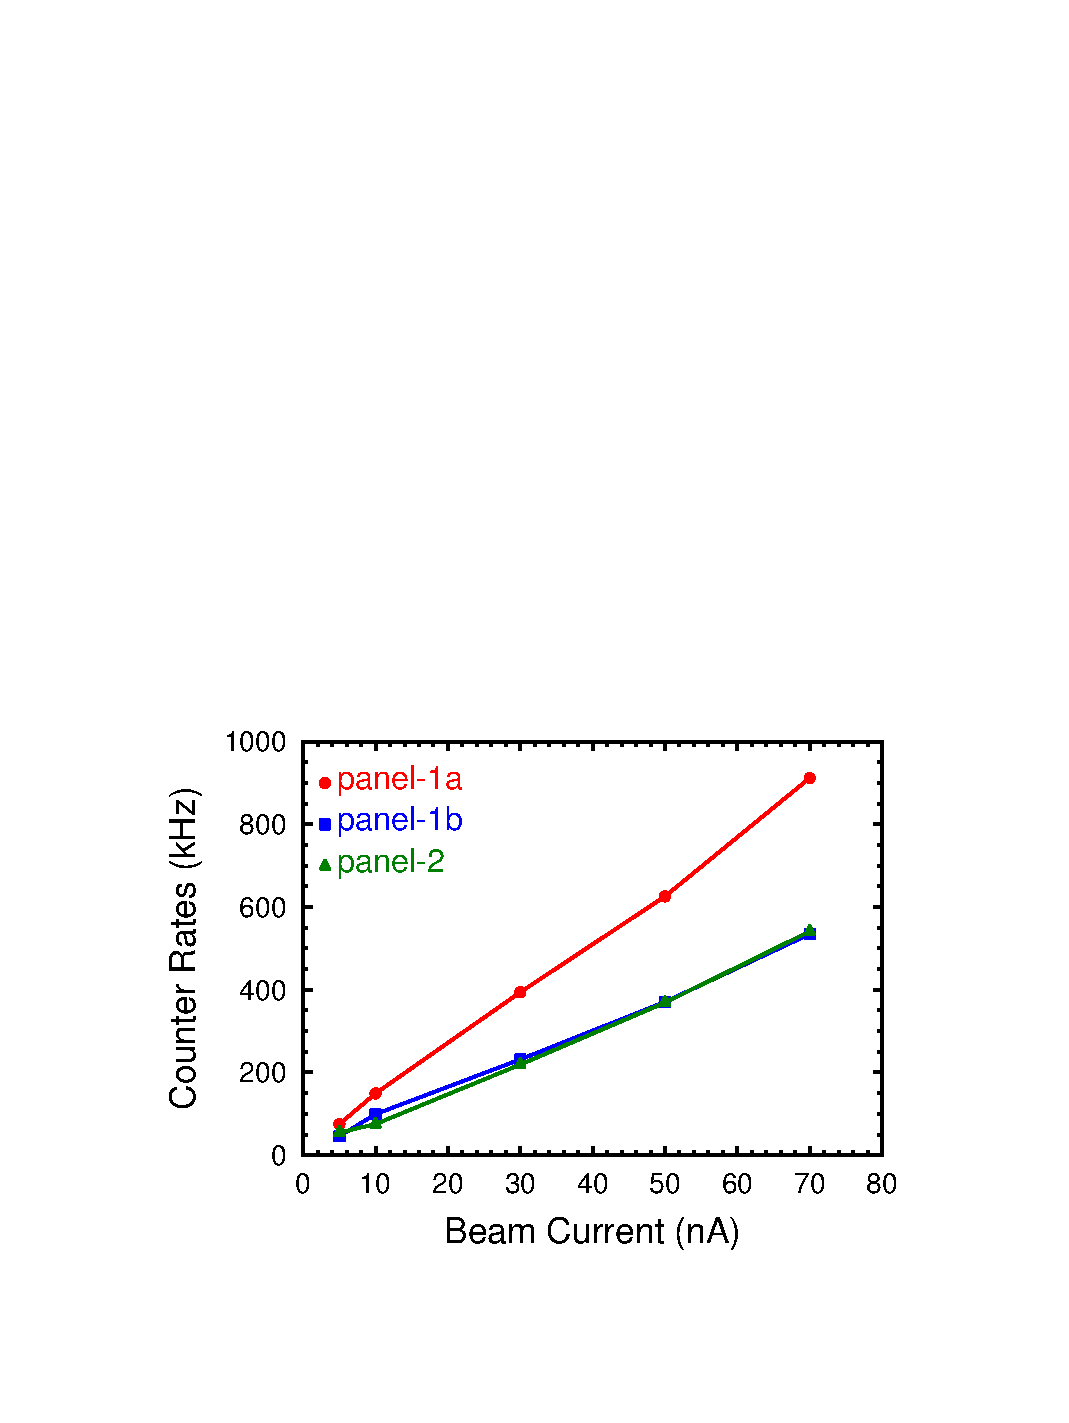
\includegraphics[width=1.2\textwidth,natwidth=610,natheight=642]{pics/ftof-rates.pdf}}}
\end{picture} 
\caption{(Color Online) FTOF counter rates (kHz) for 11~GeV electrons on a liquid-hydrogen target
as a function of beam current (nA). The nominal operating luminosity of CLAS12 of $1 \times 10^{35}$
cm$^{-2}$s$^{-1}$ corresponds to a beam current of $\sim$70~nA. The red circles correspond to the
average panel-1a counter rates, the blue squares correspond to the average panel-1b counter rates, and
the green triangles correspond to the average panel-2 counter rates.}
\label{ftof-rates}
\end{figure}
%%%%%%%%%%%%%%%%%%%%%%%%%%%%%%%%%%%%%%%%%%%%%%%%%%%%%%%%%

Based on a detailed simulation of the full CLAS12 detector and beamline based on our GEANT-4 Monte
Carlo~\cite{clas12-gemc}, the response of the FTOF with an 11~GeV electron beam incident upon a 5~cm
liquid-hydrogen target has been studied. Shown in Fig.~\ref{ftof-gemc} is a comparison of the contributions
to the overall rate associated with hits above the readout threshold separated into contributions from
photons, neutrons, and charged hadrons. By far the dominant contribution to the overall measured FTOF rate
is associated with low energy photons whose energy deposition in the counters is significantly less than the
contribution from minimum-ionizing hadrons.

%%%%%%%%%%%%%%%%%%%%%%%%%%%%%%%%%%%%%%%%%%%%%%%%%%%%%%%%%
\begin{figure}[ht]
\vspace{1.0cm}
\begin{picture}(50,50) 
\put(60,180)
{\hbox{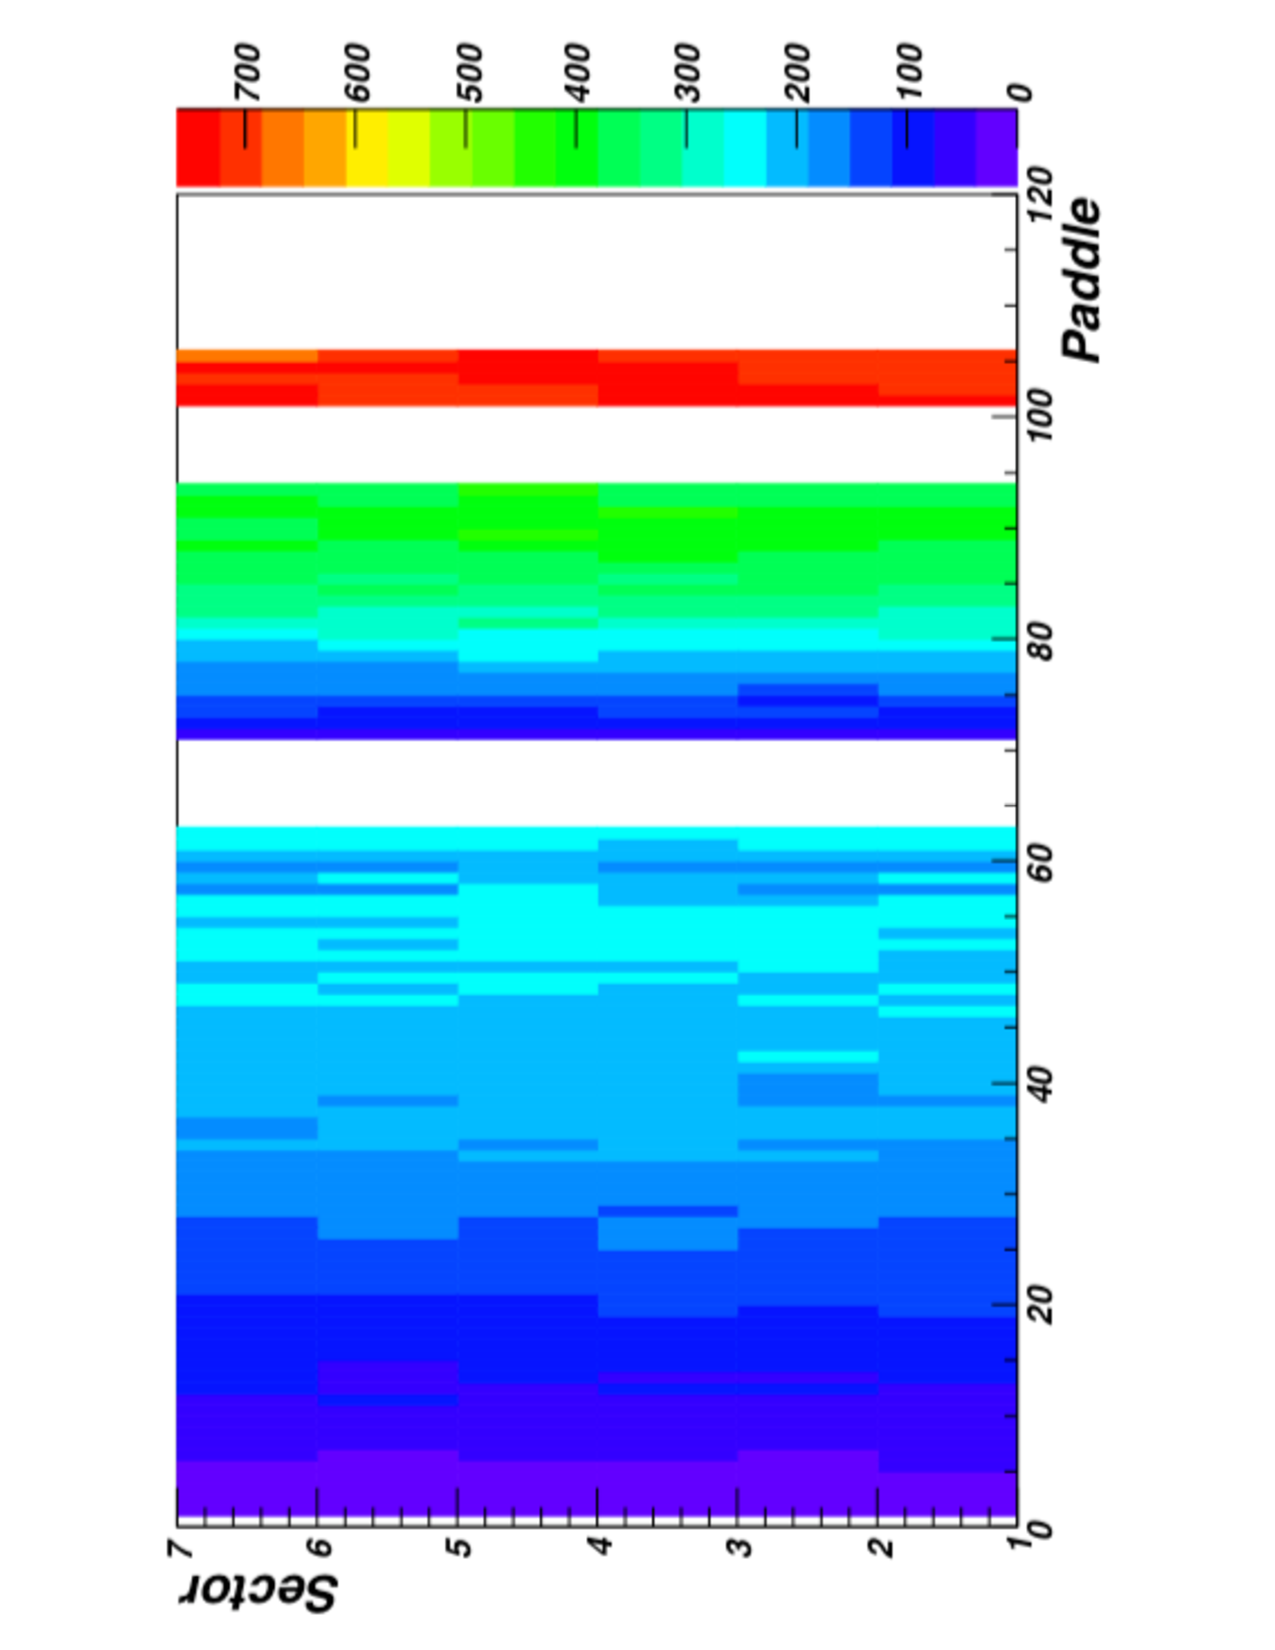
\includegraphics[width=0.54\textwidth,natwidth=610,natheight=642,angle=-90]{pics/mc-rates.pdf}}}
\end{picture} 
\put(280,145){(kHz)}
\caption{(Color Online) Simulation results for the FTOF counter rates (kHz) for 11~GeV electrons on a
liquid-hydrogen target at the nominal CLAS12 design luminosity of $1 \times 10^{35}$~cm$^{-2}$s$^{-1}$.
The rates are calculated for a 1~MeV threshold on deposited energy and expressed in kHz. Here the
leftmost group of 62 paddles corresponds to panel-1b, the middle group of 23 paddles corresponds to
panel-1a, and the rightmost group of 5 paddles corresponds to panel-2.}
\label{ftof-gemc}
\end{figure}
%%%%%%%%%%%%%%%%%%%%%%%%%%%%%%%%%%%%%%%%%%%%%%%%%%%%%%%%%

The average PMT current is directly proportional to the average number of photoelectrons $\langle N_{phe} \rangle$ 
created at the photocathode by the scintillation light and the average incident charged particle event rate 
$\langle R \rangle$. This current can be expressed as:

\begin{equation}
\langle i_{PMT} \rangle = \langle N_{phe} \rangle \cdot Q_e \cdot G \cdot \langle R \rangle,
\end{equation}

\noindent
where $Q_e = 1.6 \times 10^{-19}$ C/e is the electron charge, $G$ is the PMT gain (assumed to be
$1 \times 10^6$, and $R$ is the rate per bar. Using the photoelectron statistics estimated detailed in
Section~\ref{res-sec}, Fig.~\ref{mc-pmt-currents} shows the predictions of the PMT anode currents
for all of the FTOF counters at nominal operating luminosity at 11~GeV from our detailed GEANT-4 Monte
Carlo studies~\cite{gemc-cn2017}. These predictions show typical PMT anode currents in the panel-1a and
panel-1b PMTs at the level of 5~$\mu$A to 10~$\mu$A increasing linearly with counter length. Direct
measurements in beam of the PMT anode currents were made as shown in Fig.~\ref{pmt-currents}. The
measurements from beam are in very good accord with the simulation expectations.

%%%%%%%%%%%%%%%%%%%%%%%%%%%%%%%%%%%%%%%%%%%%%%%%%%%%%%%%%
\begin{figure}[htbp]
\vspace{3.6cm}
\begin{picture}(50,50) 
\put(45,185)
{\hbox{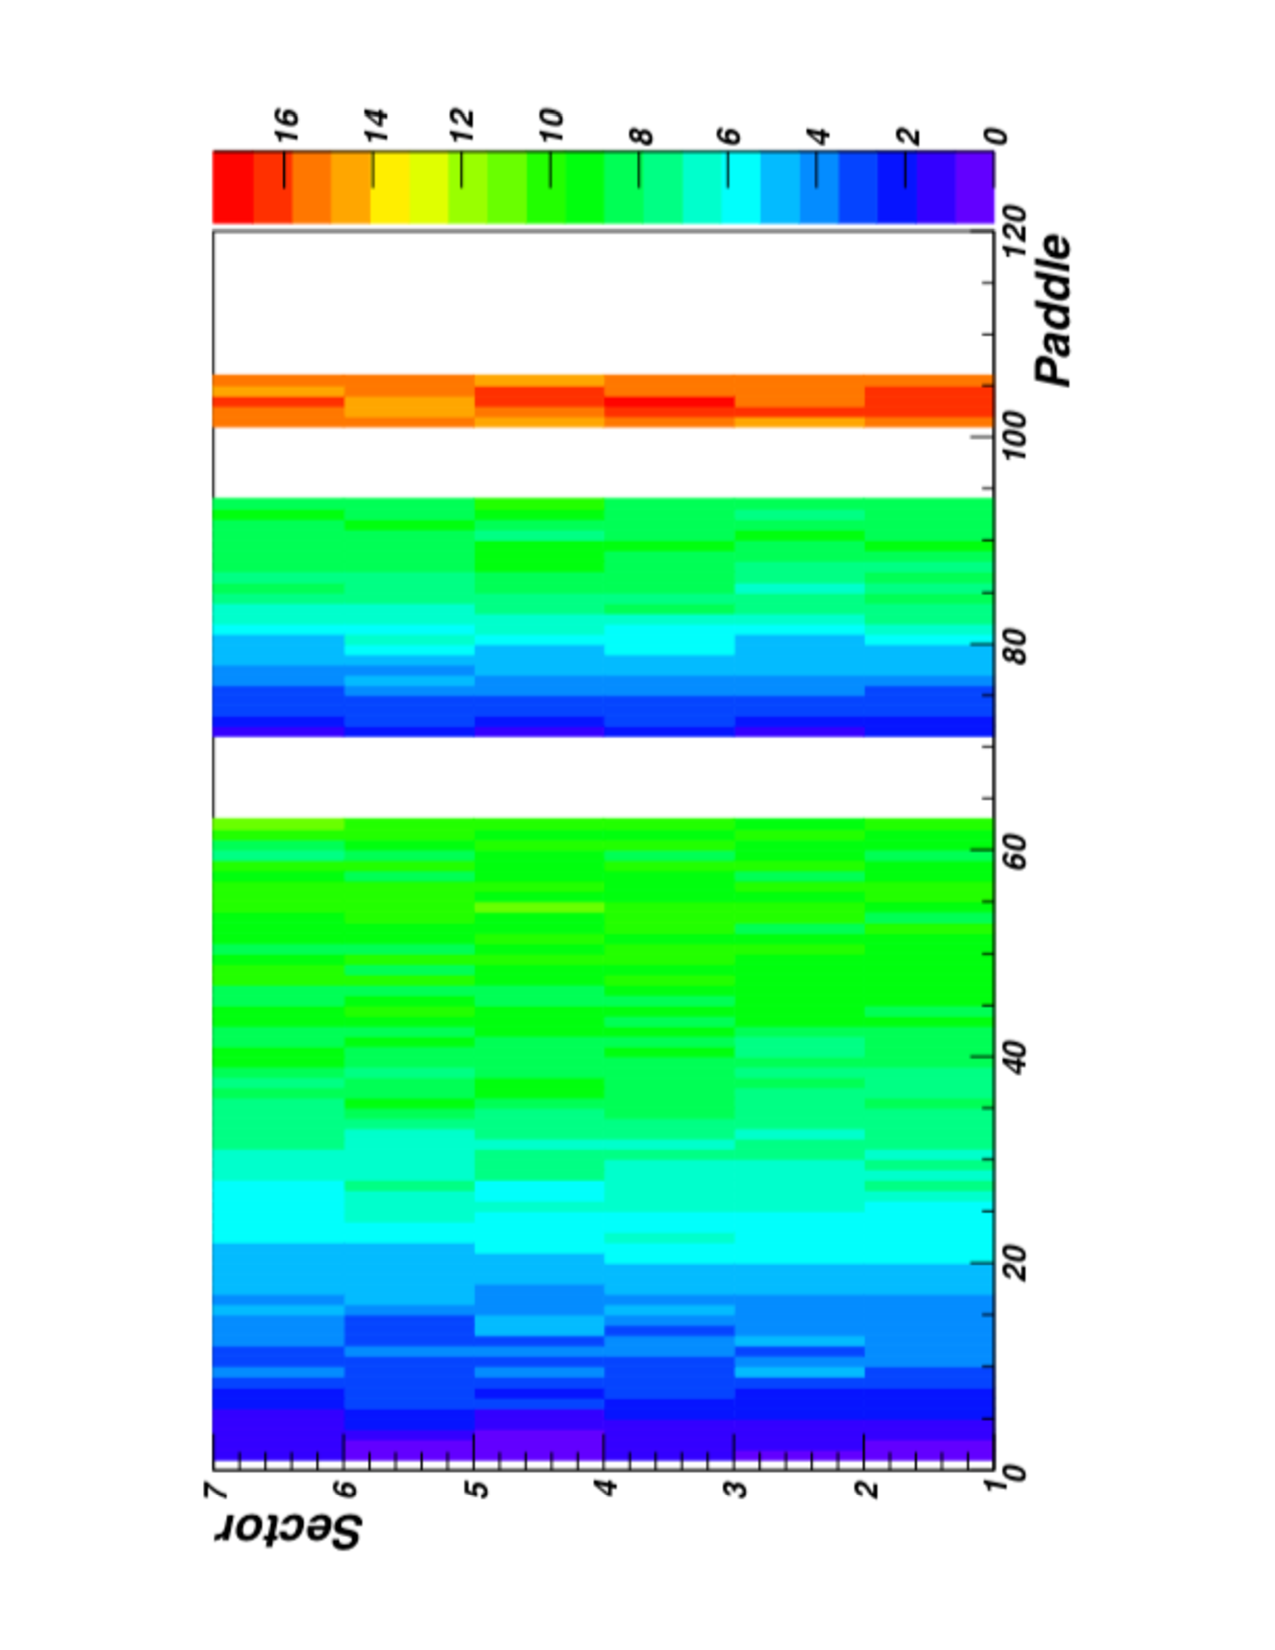
\includegraphics[width=0.57\textwidth,natwidth=610,natheight=642,angle=-90]{pics/mc-currents.pdf}}}
\put(320,145){($\mu$A)}
\end{picture} 
\caption{(Color Online) Computed PMT currents from Monte Carlo studies at the nominal operating luminosity
of CLAS12 of $1 \times 10^{35}$~cm$^{-2}$s$^{-1}$ with 11~GeV electrons incident upon a liquid-hydrogen
target. Here the leftmost group of 62 paddles corresponds to panel-1b, the middle group of 23 paddles
corresponds to panel-1a, and the rightmost group of 5 paddles corresponds to panel-2.}
\label{mc-pmt-currents}
\end{figure}
%%%%%%%%%%%%%%%%%%%%%%%%%%%%%%%%%%%%%%%%%%%%%%%%%%%%%%%%%

%%%%%%%%%%%%%%%%%%%%%%%%%%%%%%%%%%%%%%%%%%%%%%%%%%%%%%%%%
\begin{figure}[htbp]
\vspace{4.2cm}
\begin{picture}(50,50) 
\put(60,-70)
{\hbox{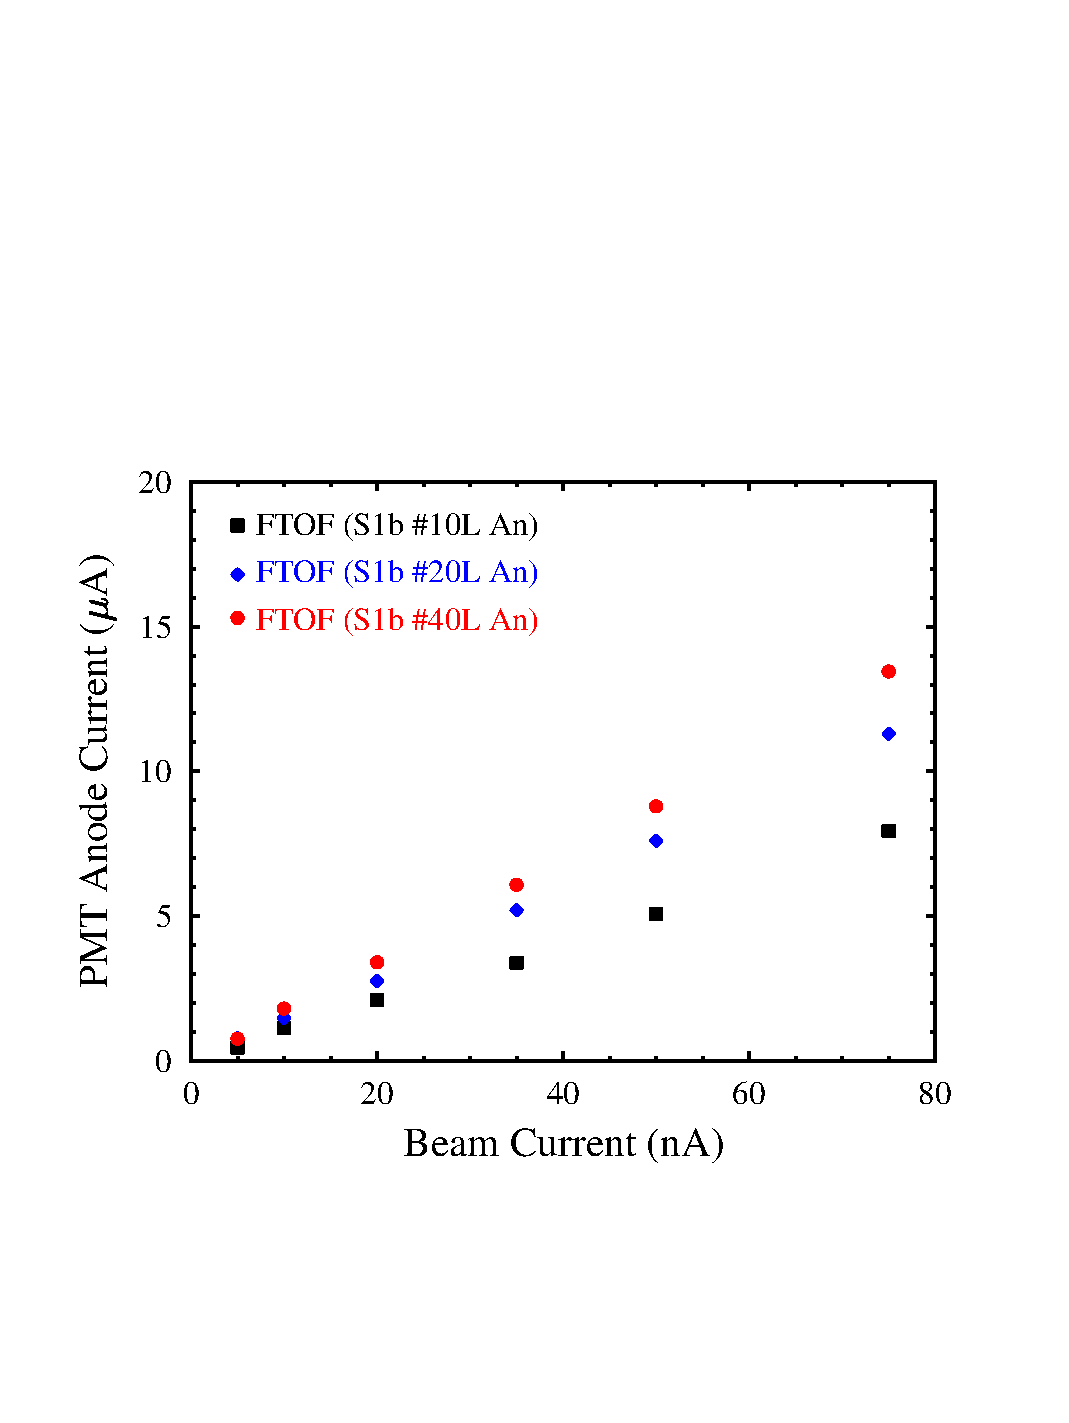
\includegraphics[width=0.8\textwidth,natwidth=610,natheight=642]{pics/full-ftof.pdf}}}
\end{picture} 
\caption{(Color Online) Measurements of the PMT anode current for representative panel-1b PMTs
 ($N_{counter}=10, 20, 40$) as a function of beam current with a 10.6~GeV electron incident upon a
5~cm liquid-hydrogen target.}
\label{pmt-currents}
\end{figure}
%%%%%%%%%%%%%%%%%%%%%%%%%%%%%%%%%%%%%%%%%%%%%%%%%%%%%%%%%

\subsubsection{Reconstruction Results}

Particle identification in the Forward Detector of CLAS12 relies heavily on the combination of measured
charged particle momenta and the flight time from the target to the respective FTOF counters. The vertex
time is determined with respect to the accelerator RF, modulo the RF period $T_{RF}$. The beam bucket for
each event is identified using the flight time of scattered electrons or high-momentum pions, traced back to
the interaction point. The FTOF resolution of $< 200$~ps allows clear selection of the correct beam bucket. In
Fig.~\ref{fig:masses} we show the distribution of masses for all reconstructed positively charged hadrons
without any kinematic cuts other than those imposed by the detector acceptance for the data taken with a
10.6~GeV electron beam incident upon a liquid-hydrogen target and after initial calibrations of the FTOF system.
A clear separation of pions and protons can be seen from these data. For these data the $RF$ period was 4.008~ns.

%%%%%%%%%%%%%%%%%%%%%%%%%%%%%%%%%%%%%%%%%%%%%%%%%%%%%%%%%
\begin{figure}[htbp]
\vspace{3.3cm}
\begin{picture}(50,50) 
\put(1,325)
{\hbox{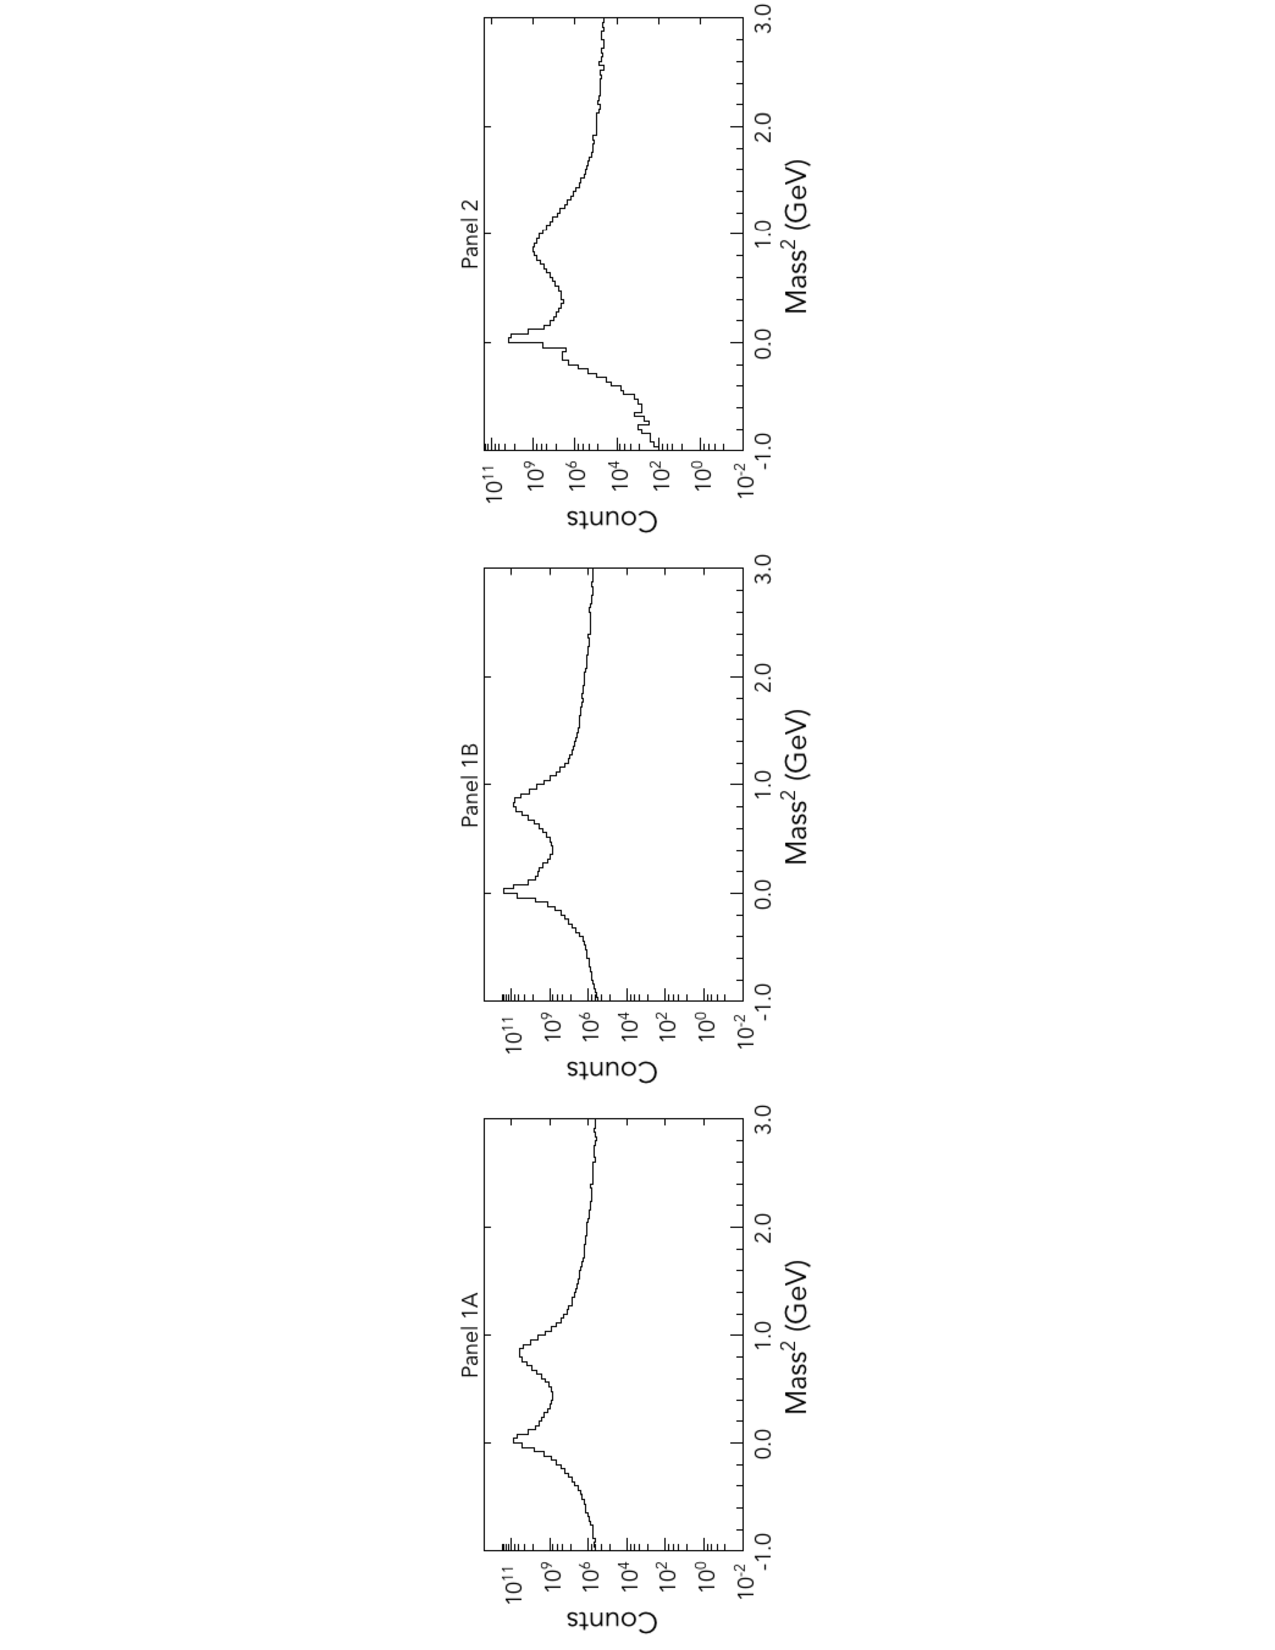
\includegraphics[width=1.3\textwidth,height=0.48\textheight,natwidth=610,natheight=642,angle=-90]
{pics/ftof-mass.pdf}}}
\end{picture} 
\caption{Reconstructed mass squared (GeV$^2$) for positively charged particles for all counters in panel-1a
(left), panel-1b (middle), and panel-2 (right) from beam data with a 10.6~GeV electron incident on a
liquid-hydrogen target.}
\label{fig:masses}
\end{figure}
%%%%%%%%%%%%%%%%%%%%%%%%%%%%%%%%%%%%%%%%%%%%%%%%%%%%%%%%

A plot of velocity versus momentum is shown in Fig. \ref{fig:betavsp} for positively charged particles, displaying
the overall particle identification possible with this detector through the separation of the different particle
species. Here the distributions are presented separately for the counters in panel-1a, panel-1b, and panel-2 summed
over all CLAS12 Forward Detector sectors. These distributions qualitatively show the particle separation for
$\pi/K$, $\pi/p$, and $K/p$ vs. momentum as required by the system specifications in Section~\ref{sec:overview}
and Table~\ref{spec-table}.

%%%%%%%%%%%%%%%%%%%%%%%%%%%%%%%%%%%%%%%%%%%%%%%%%%%%%%%%%
\begin{figure}[htbp]
\vspace{3.7cm}
\begin{picture}(50,50) 
\put(-32,-155)
{\hbox{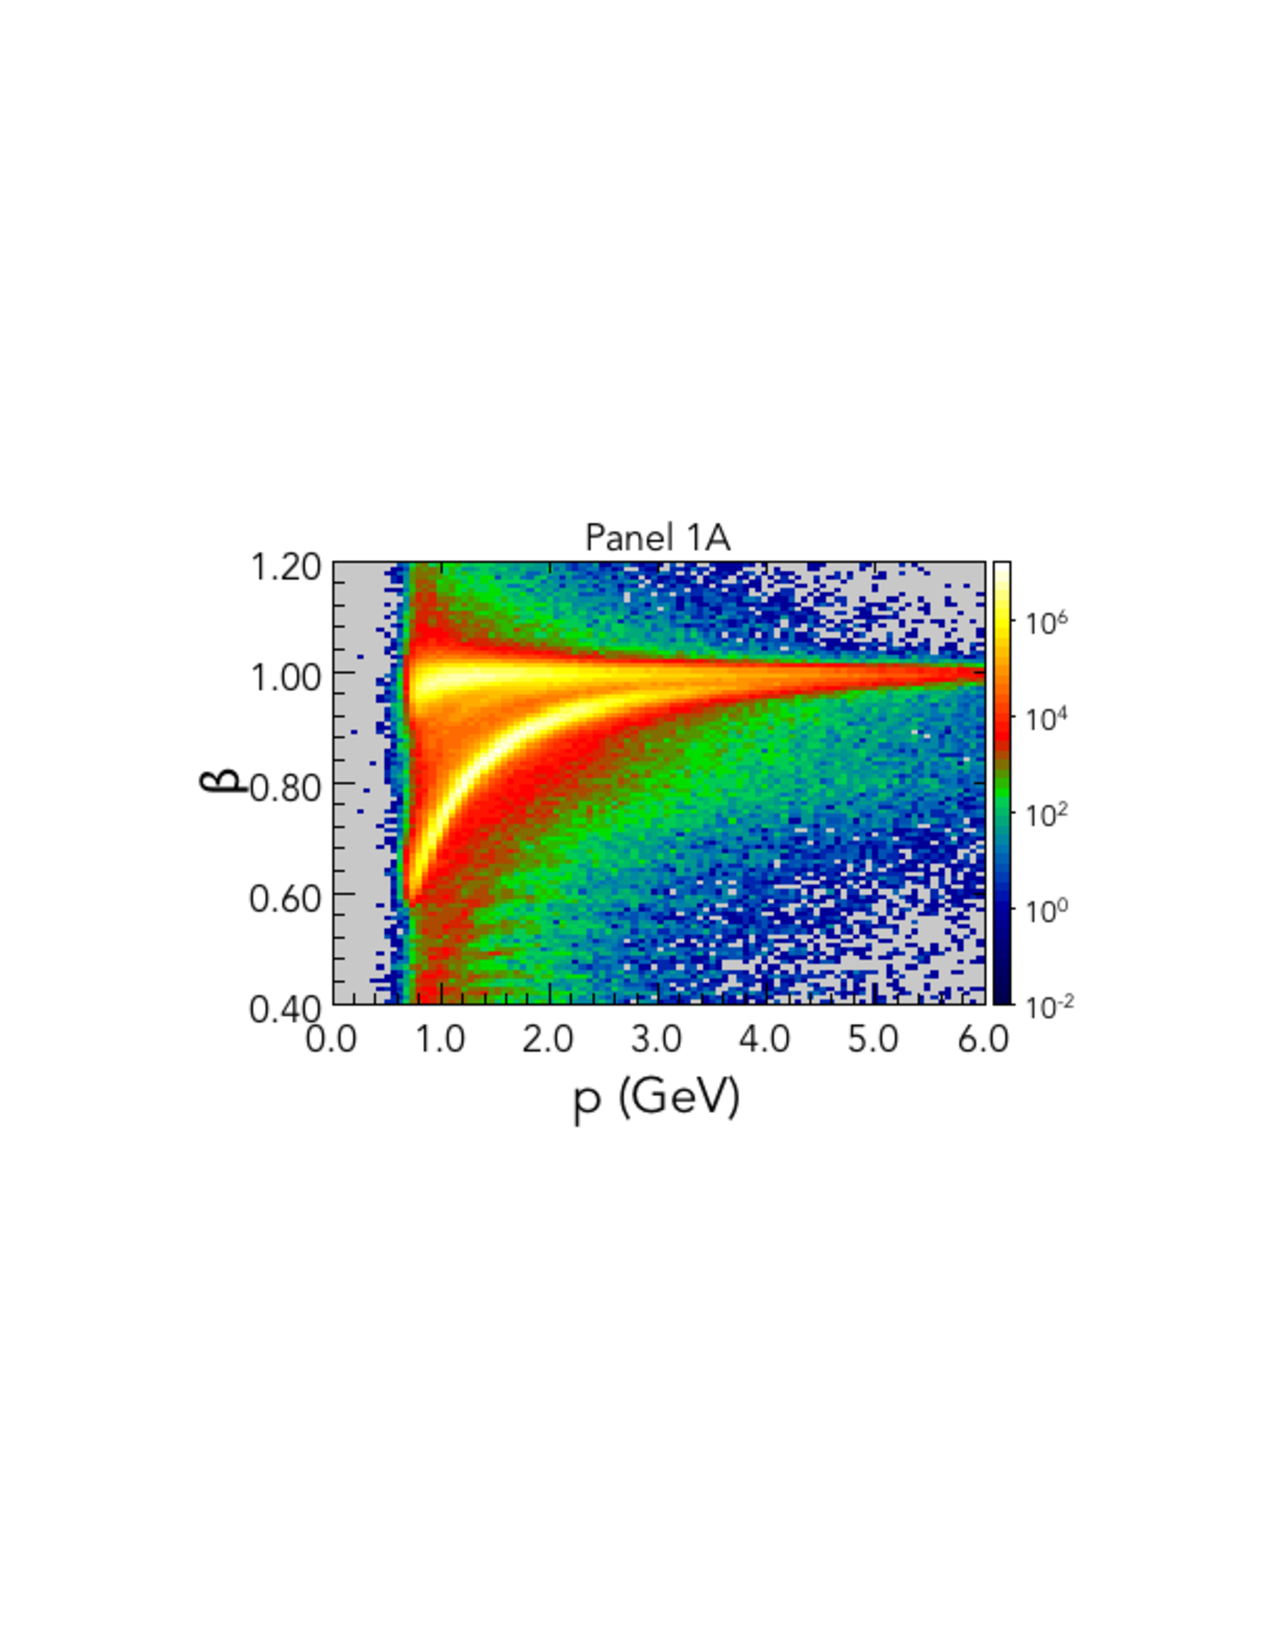
\includegraphics[width=0.47\textwidth,height=0.58\textheight,natwidth=610,natheight=642]{pics/p1a-bvsp.pdf}}}
\put(103,-155)
{\hbox{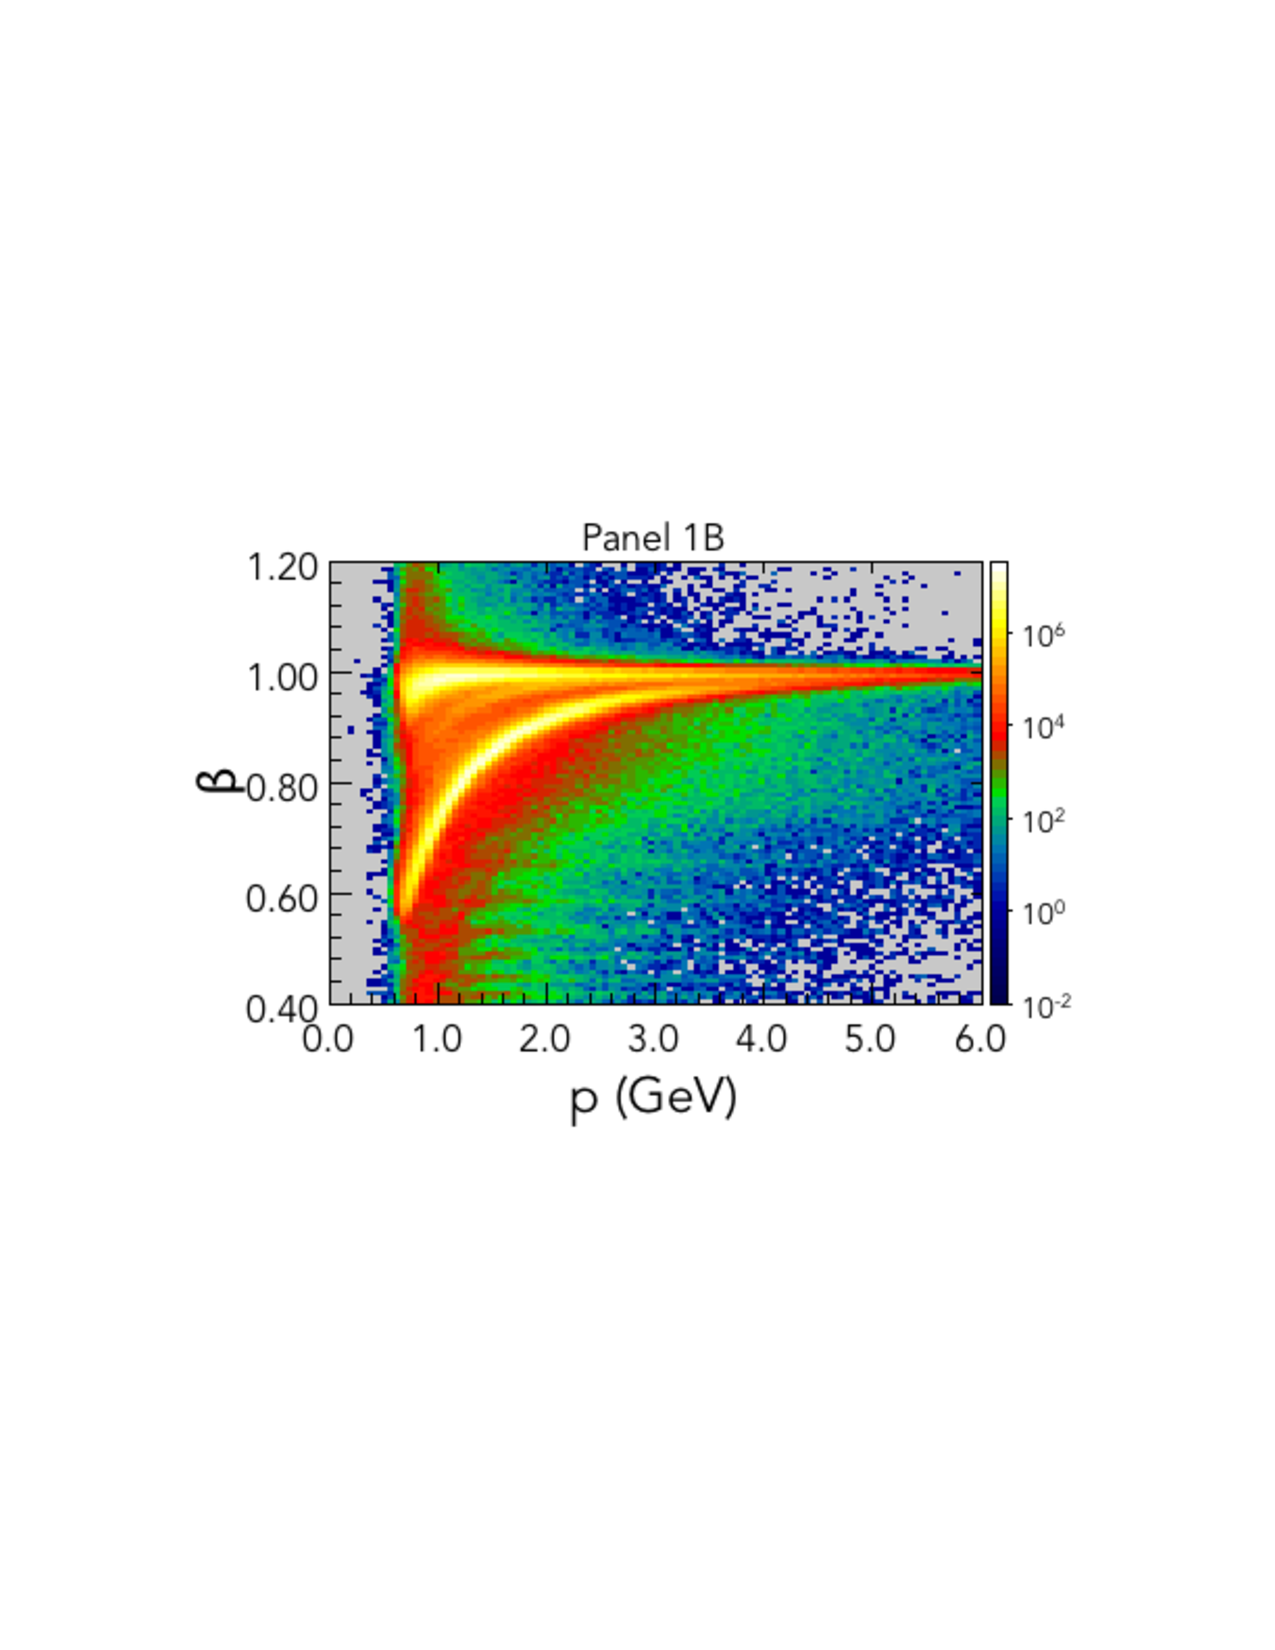
\includegraphics[width=0.47\textwidth,height=0.58\textheight,natwidth=610,natheight=642]{pics/p1b-bvsp.pdf}}}
\put(238,-155)
{\hbox{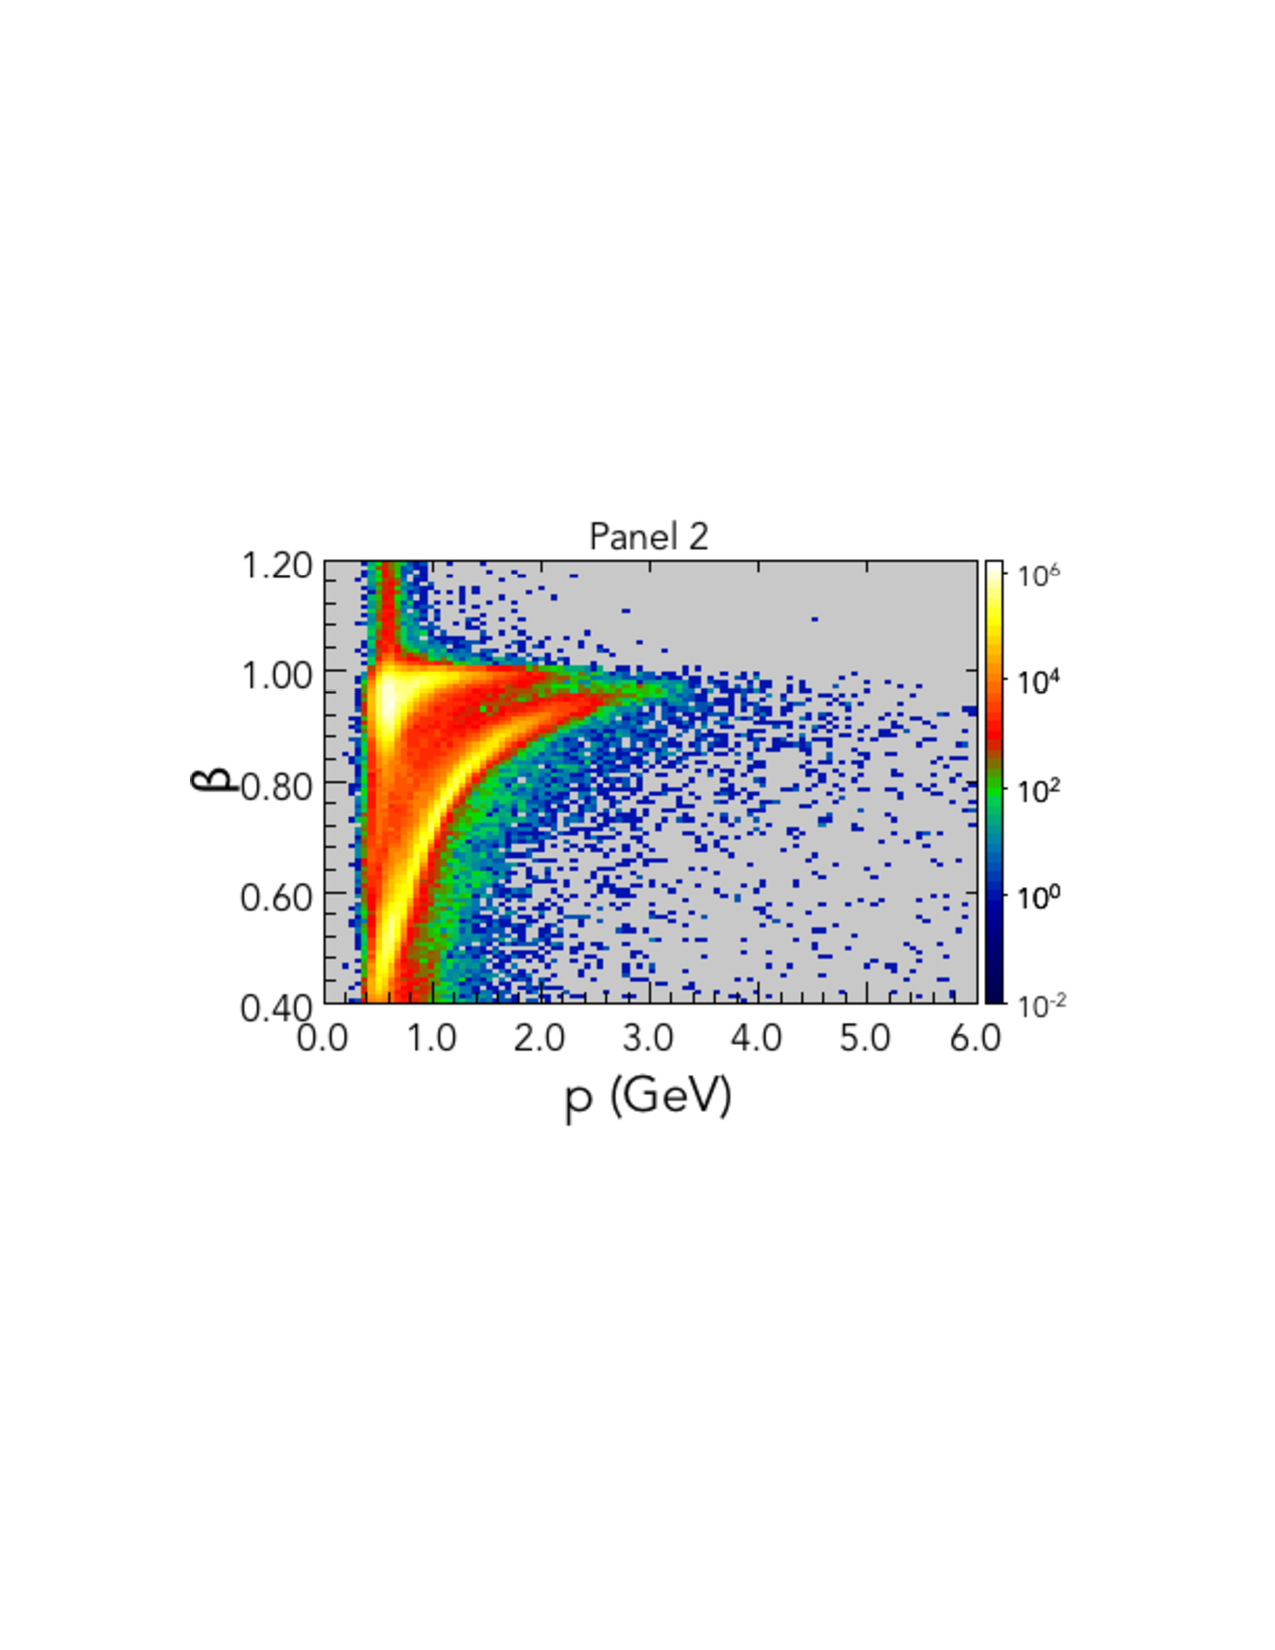
\includegraphics[width=0.47\textwidth,height=0.58\textheight,natwidth=610,natheight=642]{pics/p2-bvsp.pdf}}}
\end{picture} 
\caption{(Color Online) Velocity of positive hadrons ($\beta$) versus momentum (GeV) for all counters in
panel-1a (left), panel-1 (middle), and panel-2 (right) from beam data with a 10.6~GeV electron incident on
a liquid-hydrogen target.}
\label{fig:betavsp}
\end{figure}
%%%%%%%%%%%%%%%%%%%%%%%%%%%%%%%%%%%%%%%%%%%%%%%%%%%%%%%%%%

\section{Summary}
\label{sec:summary}

We have designed and assembled a time-of-flight system for the Forward Detector of the new CLAS12
Spectrometer in Hall~B at Jefferson Lab known as the Forward Time-of-Flight or FTOF detector. This
system consists of 88 scintillation bars in each of the six forward sectors of the CLAS12 Forward Detector
for a total of 540 counters. This design is based on rectangular counters varying in length from 17~cm long
to 426~cm long in three different counter arrays in each sector. In the polar angle range from 5$^\circ$ to
35$^\circ$ the FTOF system consists of two layers of counters referred to as the panel-1a counters and the
panel-1b counters. The panel-1a counters were refurbished from the forward TOF counters that were part
of the original CLAS spectrometer. The panel-1b counters were newly constructed for CLAS12. Together the
timing measurements from these counters provide time resolutions over all bars from 60~ps for the short
counters at small angles to 100~ps for the long counters at large angles. In the polar angle range from
35$^\circ$ to 45$^\circ$ the FTOF system consists of the panel-2 counters that provide timing resolutions
of $\sim$200~ps. With these timing resolutions the FTOF system can separate $\pi/K$ to 2.8~GeV, $K/p$
to 4.8~GeV, and $\pi/p$ to 5.4~GeV with 4$\sigma$ separation with up to an order of magnitude difference
in the relative yields.  The specifications are sufficient to meet to meet the particle identification requirements
in the forward direction for the full CLAS12 physics program. The performance of the FTOF system was
verified in extensive bench studies in our cosmic ray test stands as well as after installation in the first beam
runs with the CLAS12 system in the period from Dec. 2017 to May 2018. 

\ack

We benefited greatly from useful discussions with and assistance from Sergey Boyarinov, Chris Cuevas,
Haiyan Lu, Cole Smith, Elton Smith, and Veronique Ziegler. We also thank the Hall~B technical crew for their
efforts during counter installation and cabling. This work was supported in part by DOE Contract
\#DE-AC05-84ER40150.

\newpage

\begin{thebibliography}{99}

\bibitem{clas-nim}
B.A. Mecking {\it et al.}, Nucl. Inst. and Meth. {\bf A503}, 513 (2003).

\bibitem{clas12-nim}
V.D. Burkert {\it et al.}, to be published in Nucl. Inst. and Meth. A, (2020).
  
\bibitem{tof-nim}
E.S. Smith {\it et al.}, Nucl. Inst. and Meth. {\bf A432}, 265 (1999).

\bibitem{bicron}
Bicron, 12345 Kinsman Road, Newbury, OH 44065, http://www.bicron.com.

\bibitem{hamamatsu}
Hamamatsu Photonics, http://www.hamamatsu.com.
  
\bibitem{nim-p1b}
R. Gothe, {\it A New Time-of-Flight System for CLAS12''}, to be submitted to Nucl. Inst. and Meth A, (2020).

\bibitem{ftof-geom}
D.S. Carman, {\it Forward Time-of-Flight Geometry for CLAS12}, CLAS12-Note 2014-005.
https://misportal.jlab.org/mis/physics/clas12/viewFile.cfm/2014-005.pdf?documentId=13

\bibitem{kuhlen}
M. Kuhlen, M. Moszynski, R. Stroynowski, E. Wicklund, and B. Milliken, Nucl.  Instr. and Meth.
{\bf A301}, 223 (1991).

\bibitem{scint-mat-ref}
https://www.crystals.saint-gobain.com/sites/imdf.crystals.com/files/documents/bc400-404-408-412-416-data-sheet.pdf

\bibitem{et-ref}
ADIT Electron Tubes, 300 Crane St, Sweetwater, TX 79556
  
\bibitem{photonis}
Photonis Imaging Sensors, http://www.photonis.com

\bibitem{ftof-shields}
D.S. Carman and V. Baturin, {\it CLAS12 FTOF Studies: Rate and Magnetic Shielding Effects on PMT Timing
Resolutions}, CLAS-Note 2011-018.\\
https://misportal.jlab.org/ul/Physics/Hall-B/clas/viewFile.cfm/2011-018.pdf?documentId=653
  
\bibitem{tdc-manual}
http://www.caen.it/servlet/checkCaenManualFile?Id=12125
  
\bibitem{inl-tables}
E. Jastremski, https://www.jlab.org/Hall-B/ftof/manuals/caen-inl-notes.pdf

\bibitem{fadc-manual}
https://www.jlab.org/Hall-B/ftof/manuals/FADC250UsersManual.pdf
  
\bibitem{epics}
EPICS (Experimental Physics and Industrial Control System),\\ http://www.aps.anl.gov/epics

\bibitem{dsc-cn2013-001}
D.S. Carman, {\it CLAS12 FTOF Panel-1a and Panel-2 Refurbishment and Baseline Test Results}, CLAS12-Note 2013-001.\\
https://misportal.jlab.org/mis/physics/clas12/viewFile.cfm/2013-001.pdf?documentId=1

\bibitem{Gi86} 
R.T. Giles, F.M. Pipkin, and J.P. Wolinski, Nucl. Instr. and Meth. A {\bf 252}, 41 (1986).

\bibitem{kajino}
T. Yamaoka, F. Kajino, I. Tada, S. Hayashi, {\it Absolute Number Calibration of Photoelectrons of
Photomultiplier Tubes Using the Nature of Statistical Distribution}, Proceedings of the 28th International
Cosmic Ray Conference, July 31 - August 7, 2003, editors: T. Kajita, Y. Asaoka, A. Kawachi, Y. Matsubara, and
M. Sasaki, p. 2871 (2003).

\bibitem{pmt-currents}
D.S. Carman, {\it Forward Time-of-Flight PMT Currents}, FTOF internal note, (2014).
https://www.jlab.org/Hall-B/ftof/notes/ftof\_currents.pdf

\bibitem{ftof-calib}
D.S. Carman, {\it Description of the Calibration Algorithms for the CLAS12 Forward Time-of-Flight System},\\
https://www.jlab.org/Hall-B/ftof/notes/ftof\_calib.pdf

\bibitem{ftof-recon}
D.S. Carman, {\it Forward Time-of-Flight Reconstruction for CLAS12},\\
https://www.jlab.org/Hall-B/ftof/notes/ftof-recon.pdf

\bibitem{clas12-gemc}
CLAS12 GEANT4 Monte Carlo suite {\it gemc}, http://gemc.jlab.org.

\bibitem{gemc-cn2017}
R. De Vita, D.S. Carman, C. Smith, S. Stepanyan, and M. Ungaro, {\it Study of the Electromagnetic Background
Rates in CLAS12}, CLAS12-Note 2017-016.\\
https://misportal.jlab.org/mis/physics/clas12/viewFile.cfm/2017-016.pdf?documentId=52

%\bibitem{scint-spec}
%Eljen Technologies scintillator specifications,\\
%http://www.eljentechnology.com/images/technical\_library/Physical\_Constants\_Plastic.pdf

\end{thebibliography}

\end{document}
